\newpage
\thispagestyle{empty}
\setcounter{chapter}{8}
\pdfbookmark[0]{Chapter 8 Laplace Transforms}{chapter:8}
\chaptertitle{Laplace Transforms}

\noindent
IN THIS CHAPTER
 we study the method of
\href{http://www-history.mcs.st-and.ac.uk/Mathematicians/Laplace.html}
{\color{blue}\it Laplace
 transforms}, which illustrates one of
 the basic problem solving techniques in mathematics:
transform a difficult problem into an easier one, solve the latter,
and then use its solution to obtain a solution of the original
problem. The method discussed here
transforms an initial value problem for a constant coefficient
equation into an algebraic equation whose solution can then be used to
solve the initial value problem. In some cases this method is merely
an alternative procedure for solving problems that can be solved
equally well by methods that we considered previously;     however,
in other cases  the method of Laplace transforms is more efficient
than the methods previously discussed. This is especially true
in physical problems dealing with discontinuous forcing functions.

\medskip
\noindent
SECTION~8.1  defines  the Laplace transform and
developes its properties.

\medskip
\noindent
SECTION~8.2 deals with
the problem of finding a function that has a given Laplace transform.

\medskip
\noindent
 SECTION~8.3 applies the Laplace transform to solve
initial value problems for constant coefficient second order
differential equations on $(0,\infty)$.

\medskip
\noindent
SECTION~8.4
introduces the unit step function.

\medskip
\noindent
SECTION~8.5 uses the unit step function
 to solve constant coefficient equations with piecewise
continuous forcing functions.

\medskip
\noindent
SECTION~8.6 deals with the
convolution theorem, an important theoretical property of the Laplace
transform.

\medskip
\noindent
 SECTION~8.7 introduces the idea of
impulsive force, and treats constant coefficient equations with
impulsive forcing functions.

\medskip
\noindent
SECTION~8.8 is a brief table of Laplace transforms.

\vspace*{2in}
\centerline{393}
\newpage

\section{Introduction to the Laplace Transform}

\noindent
\boxit{Definition of the Laplace Transform}

\noindent
To define the Laplace transform, we first recall the definition of an
improper integral. If $g$ is integrable over the
interval $[a,T]$ for every $T>a$, then the {\color{blue}\it improper
integral of
$g$ over\/} $[a,\infty)$ is defined as
\begin{equation} \label{eq:8.1.1}
\int^\infty_a g(t)\,dt=\lim_{T\to\infty}\int^T_a g(t)\,dt.
\end{equation}
We say that the improper integral {\color{blue}\it converges\/} if the limit in
\eqref{eq:8.1.1} exists;   otherwise, we say that the improper integral
{\color{blue}\it
diverges\/} or {\color{blue}\it does not exist\/}. Here's the definition of
the Laplace transform of a function $f$.

\begin{definition}\color{blue}\label{thmtype:8.1.1}\rm
Let $f$ be defined for $t\ge0$ and let $s$ be a real number. Then the
\href{https://mathshistory.st-andrews.ac.uk/Biographies/Laplace/}
{\color{blue}\it Laplace transform} of $f$ is the function $F$ defined by
\begin{equation}\label{eq:8.1.2} F(s)=\int_0^\infty e^{-st} f(t)\,dt,
\end{equation} for those values of $s$ for which the improper integral
converges.
\end{definition}

It is important to keep in mind that the variable of integration in
\eqref{eq:8.1.2} is $t$, while $s$ is a parameter independent of $t$. We
use $t$ as the independent variable for $f$ because in applications
the Laplace transform is usually applied to functions of time.

The Laplace transform can be viewed as an operator ${\cal L}$ that
transforms the function $f=f(t)$  into the function $F=F(s)$. Thus,
\eqref{eq:8.1.2} can be expressed as
$$
F={\cal L}(f).
$$
The functions $f$ and $F$ form a {\color{blue}\it transform pair\/}, which we'll
sometimes denote by
$$
f(t)\leftrightarrow F(s).
$$
It can be shown that if $F(s)$ is defined for $s=s_0$ then it's defined
for all $s>s_0$ (Exercise~\ref{exer:8.1.14}\part{b}).

\boxit{Computation of Some Simple Laplace Transforms}

\begin{example}\label{example:8.1.1}\rm
 Find the Laplace transform of  $f(t)=1$.
\end{example}

\solution
 From  \eqref{eq:8.1.2} with $f(t)=1$,
$$
F(s)=\int_0^\infty e^{-st}\,dt=\lim_{T\to\infty}\int_0^T e^{-st}\,
dt.
$$
If $s\ne 0$ then
\begin{equation}\label{eq:8.1.3}
\int_0^T e^{-st}dt=-{1\over s}e^{-st}\Big|_0^T={1-e^{-sT}\over s}.
\end{equation}
Therefore
\begin{equation}\label{eq:8.1.4}
\lim_{T\to\infty}\int_0^T e^{-st}dt=\left\{\begin{array}{rr}
\dst{1\over s}, &   s>0,\\
\infty, &  s<0.
\end{array}\right.
\end{equation}
If $s=0$  the integrand reduces to the constant $1$, and
$$
\lim_{T\to\infty}\int_0^T 1\,dt=\lim_{T\to\infty}\int_0^T 1\,dt=
\lim_{T\to\infty}T=\infty.
$$
Therefore $F(0)$ is undefined, and
$$
F(s)=\int_0^\infty e^{-st}dt={1\over s},\quad s>0.
$$
This result can be written in operator notation as
$$
{\cal L}(1)={1\over s},\quad s>0,
$$
or as the transform pair
$$
1\leftrightarrow{1\over s},\quad s>0.
$$

\color{blue}
\remark{
It is convenient to combine the steps of integrating from $0$ to $T$
and letting $T\to\infty$. Therefore, instead of writing \eqref{eq:8.1.3}
and \eqref{eq:8.1.4} as separate steps we write
$$
\int_0^\infty e^{-st}dt=- {1\over s} e^{-st}\Big|_0^\infty=
\left\{\begin{array}{rr}\dst{1\over s}, & s>0,\\\infty,&s<
0.\end{array}\right.
$$
We'll follow this practice throughout this chapter.}
\color{black}

\begin{example}\label{example:8.1.2}\rm
 Find the Laplace transform of $f(t)=t$.
\end{example}

\solution
  From  \eqref{eq:8.1.2} with $f(t)=t$,
\begin{equation}\label{eq:8.1.5}
F(s)=\int_0^\infty e^{-st}t\,dt.
\end{equation}
If $s\ne0$,  integrating by parts yields
\begin{eqnarray*}
\int_0^\infty e^{-st}t\,dt&=&-{te^{-st}\over s}\bigg|_0^\infty
+{1\over s}\int_0^\infty e^{-st}\,dt
=-\left[{t\over s}+{1\over s^2}\right]e^{-st}\bigg|_0^\infty
\\&=&\left\{\begin{array}{rr}\dst{1\over s^2},\quad s>0,\\
\infty,\,s<0.\end{array}\right.
\end{eqnarray*}
If $s=0$, the integral in  \eqref{eq:8.1.5} becomes
$$
\int_0^\infty t\,dt={t^2\over2}\bigg|_0^\infty=\infty.
$$
Therefore $F(0)$ is undefined and
$$
F(s)={1\over s^2},\quad s>0.
$$
This result can also be written as
$$
{\cal L}(t)={1\over s^2},\quad s>0,
$$
or as the transform pair
$$
t\leftrightarrow{1\over s^2},\quad s>0.
$$

\begin{example}\label{example:8.1.3}\rm
 Find the Laplace transform of $f(t)=e^{at}$, where $a$ is a constant.
\end{example}

\solution
From  \eqref{eq:8.1.2} with $f(t)=e^{at}$,
$$
F(s)=\int_0^\infty e^{-st}e^{at}\,dt.
$$
Combining the exponentials yields
$$
F(s)=\int_0^\infty e^{-(s-a)t}\,dt.
$$
However, we know from Example~\ref{example:8.1.1}  that
$$
\int_0^\infty e^{-st}\,dt={1\over s},\quad s>0.
$$
Replacing $s$ by $s-a$ here shows that
$$
F(s)={1\over s-a},\quad s>a.
$$
This can also be written as
$$
{\cal L}(e^{at})={1\over s-a},\quad s>a, \text{\; or \; }
 e^{at}\leftrightarrow{1\over s-a},\quad s>a.
$$

\begin{example}\label{example:8.1.4}\rm
Find the Laplace transforms of $f(t)=\sin\omega t$ and
$g(t)=\cos\omega t$, where $\omega$ is a constant.
\end{example}

\solution  Define
\begin{equation}\label{eq:8.1.6}
F(s)=\int_0^\infty e^{-st}\sin\omega t\,dt
\end{equation}
and
\begin{equation}\label{eq:8.1.7}
G(s)=\int_0^\infty e^{-st}\cos\omega t\,dt.
\end{equation}
If $s>0$, integrating  \eqref{eq:8.1.6} by parts yields
$$
F(s)=-{e^{-st}\over s}\sin\omega t\Big|_0^\infty+{\omega\over s}
\int_0^\infty e^{-st}\cos\omega t\,dt,
$$
so
\begin{equation}\label{eq:8.1.8}
F(s)={\omega\over s}G(s).
\end{equation}
If $s>0$, integrating  \eqref{eq:8.1.7} by parts yields
$$
G(s)=-{e^{-st}\cos\omega t\over s}\Big|_0^\infty - {\omega\over s}
\int_0^\infty e^{-st}\sin\omega t\,dt,
$$
so
$$
G(s)={1\over s} - {\omega\over s} F(s).
$$
Now substitute from  \eqref{eq:8.1.8} into this to obtain
$$
G(s)={1\over s} - {\omega^2\over s^2} G(s).
$$
Solving this for $G(s)$ yields
$$
G(s)={s\over s^2+\omega^2},\quad s>0.
$$
This and  \eqref{eq:8.1.8} imply that
$$
F(s)={\omega\over s^2+\omega^2},\quad s>0.
$$

\boxit{Tables of Laplace transforms}

\noindent
Extensive tables of Laplace transforms have been compiled and are
commonly used in applications. The brief table of Laplace transforms
in the Appendix will be adequate for our
purposes.

\begin{example}\label{example:8.1.5}\rm  Use the
table of Laplace transforms to find  ${\cal L}(t^3e^{4t})$.
\end{example}

\solution  The table
includes the transform pair
$$
t^ne^{at}\leftrightarrow {n!\over(s-a)^{n+1}}.
$$
Setting $n=3$  and $a=4$ here yields
$$
{\cal L}(t^3e^{4t})={3!\over(s-4)^4}={6\over(s-4)^4}.\bbox
$$

We'll  sometimes write Laplace transforms of specific functions
without explicitly stating how they are obtained. In such cases you
should refer to the table of Laplace transforms.

\boxit{Linearity of the Laplace Transform}

\noindent
The next theorem presents an important property of the Laplace
transform.

\begin{theorem}\color{blue}$[$Linearity Property$]$\label{thmtype:8.1.2}
 Suppose ${\cal L}(f_i)$ is defined for
 $s>s_i$, $1\le i\le n)$.
Let $s_0$ be the largest of the numbers $s_1$, $s_{2}$, \dots,$s_n$, and
let
$c_1$, $c_2$,\dots, $c_n$ be  constants. Then
$$
{\cal L}(c_1f_1+c_2f_2+\cdots+c_nf_n)=c_1{\cal L}(f_1)+c_2{\cal L}(f_2)
+\cdots+c_n{\cal L}(f_n)\mbox{ for } s>s_0.
$$
\end{theorem}

\proof  We give the proof for the case where $n=2$. If $s>s_0$ then
\begin{eqnarray*}
{\cal L}(c_1f_1+c_2f_2)&=&
\int_0^\infty
e^{-st}\left(c_1f_1(t)+c_2f_2(t))\right)\,dt\\
&=&c_1\int_0^\infty e^{-st}f_1(t)\,dt+c_2\int_0^\infty e^{-st}f_2(t)\,dt\\
&=&c_1{\cal L}(f_1)+c_2{\cal L}(f_2).
\end{eqnarray*}

\begin{example}\label{example:8.1.6}\rm
Use  Theorem~\ref{thmtype:8.1.2} and the known Laplace transform
$$
{\cal L}(e^{at})={1\over s-a}
$$
 to find ${\cal L}(\cosh bt)\,(b\ne0)$.
\end{example}

\solution  By definition,
$$
\cosh bt={e^{bt}+e^{-bt}\over 2}.
$$
Therefore
\begin{equation}\label{eq:8.1.9}
\begin{array}{ccl}
{\cal L}(\cosh bt)&=& {\cal L}\left(\dst{1\over 2} e^{bt}+\dst{1\over
2}e^{-bt}\right)\\[2\jot]
&=&\dst{1\over 2} {\cal L}(e^{bt}) +\dst{1\over 2} {\cal L}(e^{-bt})
\qquad
\hbox{(linearity property)}\\[2\jot]
&=&\dst{1\over 2}\,\dst{1\over s-b} +\dst{1\over 2}\,\dst{1\over
s+b},
\end{array}
\end{equation}
where the first transform on the right is defined for $s>b$ and the
second
for $s>-b$; hence, both are defined for $s>|b|$.  Simplifying the
last expression in \eqref{eq:8.1.9} yields
$$
{\cal L}(\cosh bt)={s\over s^2-b^2},\quad s>|b|.
$$

\boxit{The First Shifting Theorem}

\noindent
The next theorem enables us to start with known transform pairs and derive
others. (For other results of this kind, see Exercises~\ref{exer:8.1.6}  and
\ref{exer:8.1.13}.)

\begin{theorem}\color{blue}$[$First Shifting
Theorem$]$\label{thmtype:8.1.3}
 If
\begin{equation}\label{eq:8.1.10}
F(s)=\int_0^\infty e^{-st} f(t)\,dt
\end{equation}
is the Laplace transform of $f(t)$ for $s>s_0$, then $F(s-a)$ is the
Laplace transform of $e^{at}f(t)$ for $s >s_0+a$.
\end{theorem}

{\sc Proof.} Replacing $s$ by $s-a$ in  \eqref{eq:8.1.10} yields
\begin{equation}\label{eq:8.1.11}
F(s-a)=\int_0^\infty e^{-(s-a)t}f(t)\,dt
\end{equation}
if $s-a>s_0$; that is, if $s>s_0+a$.  However,  \eqref{eq:8.1.11} can
be rewritten as
$$
F(s-a)=\int_0^\infty e^{-st}\left(e^{at}f(t)\right)\,dt,
$$
which implies the conclusion.

\begin{example}\label{example:8.1.7}\rm
  Use Theorem~\ref{thmtype:8.1.3} and the known Laplace
transforms of $1$, $t$, $\cos\omega t$, and $\sin\omega t$ to find
$$
{\cal L}(e^{at}),\quad {\cal L}(te^{at}),\quad {\cal L}(e^{\lambda t}\sin
\omega t),\mbox{and } {\cal L}(e^{\lambda t}\cos\omega t).
$$
\end{example}

\solution  In the following table the known
transform pairs  are listed on the left and  the required  transform pairs
listed on the right are obtained  by applying
Theorem~\ref{thmtype:8.1.3}.

\begin{center}
\begin{tabular}{|c|c|}\hline
$f(t)\leftrightarrow F(s)$ & $e^{at}f(t)\leftrightarrow F(s-a)$ \\\hline
&\\[9pt] $1\leftrightarrow\dst{1\over s},\quad s>0$ &
 $e^{at}\leftrightarrow\dst{1\over(s-a)},\quad s>a$\\[9pt]
  $t\leftrightarrow\dst{{1\over s^2}},\quad s>0$ &
$te^{at}\leftrightarrow\dst{{1\over(s-a)^2}},\quad s>a$\\[9pt]
$\sin\omega t\leftrightarrow\dst{{\omega\over
s^2+\omega^2}},\quad s>0$&
$e^{\lambda t}\sin\omega t\leftrightarrow\dst{{\omega\over
(s-\lambda)^2+\omega^2}},\,s>\lambda$\\[9pt]
$\cos\omega t\leftrightarrow\dst{{s\over
s^2+\omega^2}},\quad s>0$ &
$e^{\lambda t}\sin\omega t\leftrightarrow\dst{{s-\lambda\over
(s-\lambda)^2+\omega^2}},\,s>\lambda$\\[9pt]\hline
\end{tabular}
\end{center}

\boxit{Existence of Laplace Transforms}

\noindent
Not every function has a Laplace transform.  For example, it can be shown
(Exercise~\ref{exer:8.1.3}) that
$$
\int_0^\infty e^{-st}e^{t^2} dt=\infty
$$
for every real number $s$. Hence, the function $f(t)=e^{t^2}$ does not
have a Laplace transform.

Our next objective is to establish conditions that ensure the
existence of the Laplace transform of a function. We first review some
relevant definitions from calculus.

Recall that a limit
$$
\lim_{t\to t_0} f(t)
$$
exists if and only if the one-sided limits
$$
\lim_{t\to t_0-}f(t)\hbox{\quad and\quad}\lim_{t\to t_0+}f(t)
$$
  both exist and are equal;   in this case,
$$
\lim_{t\to t_0}f(t)=\lim_{t\to t_0-}f(t)=\lim_{t\to t_0+}f(t) .
$$
Recall also that $f$ is continuous at a point $t_0$ in an open interval
$(a,b)$ if and only if
$$
\lim_{t\to t_0}f(t)=f(t_0),
$$
which is  equivalent to
\begin{equation}\label{eq:8.1.12}
\lim_{t\to t_0+}f(t)=\lim_{t\to t_0-}f(t)=f(t_0).
\end{equation}
For simplicity, we  define
$$
f(t_0+)=\lim_{t\to t_0+}f(t)\quad\hbox{and }\quad f(t_0-)=\lim_{t\to
t_0-}f(t),
$$
so  \eqref{eq:8.1.12} can be expressed as
$$
f(t_0+)=f(t_0-)=f(t_0).
$$
If $f(t_0+)$ and $f(t_0-)$ have finite but distinct values,  we say
that $f$ has a {\color{blue}\it jump discontinuity\/}  at $t_0$,
 and
$$
f(t_0+)-f(t_0-)
$$
is called the {\color{blue}\it jump} in $f$ at $t_0$ (Figure~\ref{figure:8.1.1}).

\
\begin{figure}[tbp]
  \centering\color{blue}
  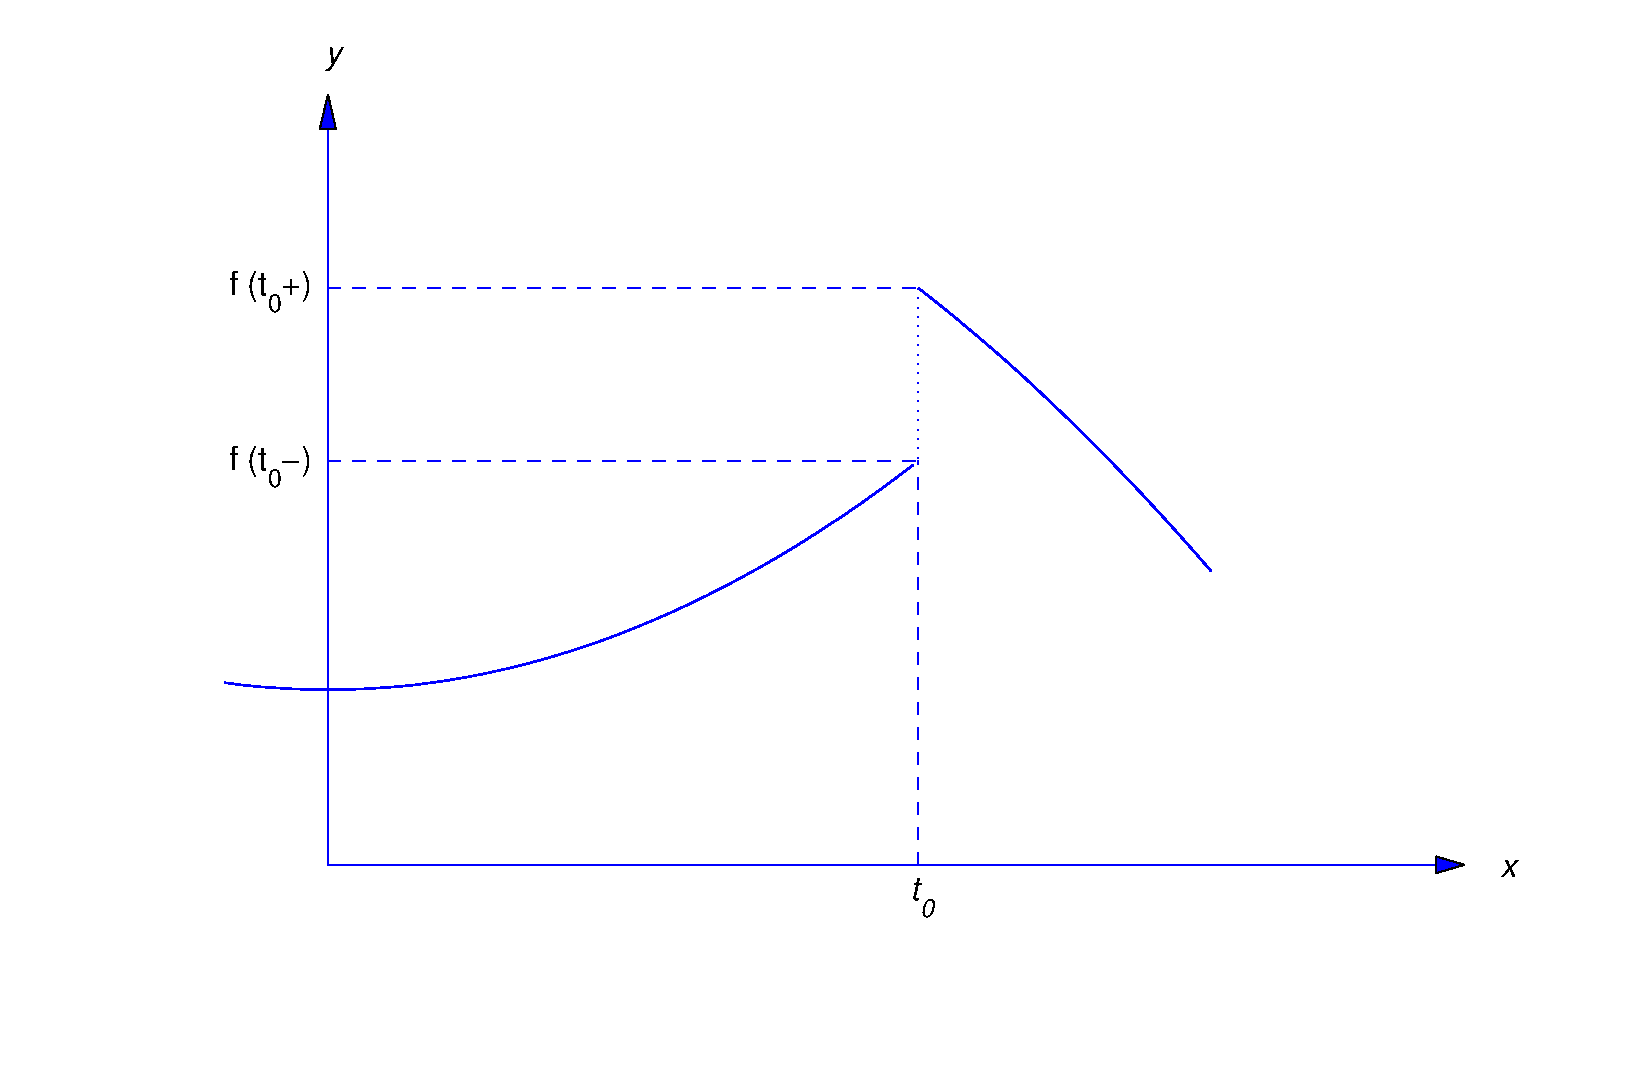
\includegraphics[bb=-78 148 689 643,width=5.67in,height=3.66in,keepaspectratio]{fig080101}
\caption{ A jump discontinuity}
  \label{figure:8.1.1}
\end{figure}

If $f(t_0+)$ and $f(t_0-)$ are finite and equal, but either $f$ isn't
defined at $t_0$ or it's defined but
$$
f(t_0)\ne f(t_0+)=f(t_0-),
$$
 we say that $f$ has a {\color{blue}\it removable discontinuity\/} at $t_0$
(Figure~\ref{figure:8.1.2}).
This terminology is appropriate since a function $f$  with a removable
discontinuity at $t_0$  can be made continuous at $t_0$ by defining (or
redefining)
$$
f(t_0)=f(t_0+)=f(t_0-).
$$

\begin{figure}[htbp]
\color{blue}
  \begin{minipage}[b]{0.5\linewidth}
    \centering
   \scalebox{.65}{
  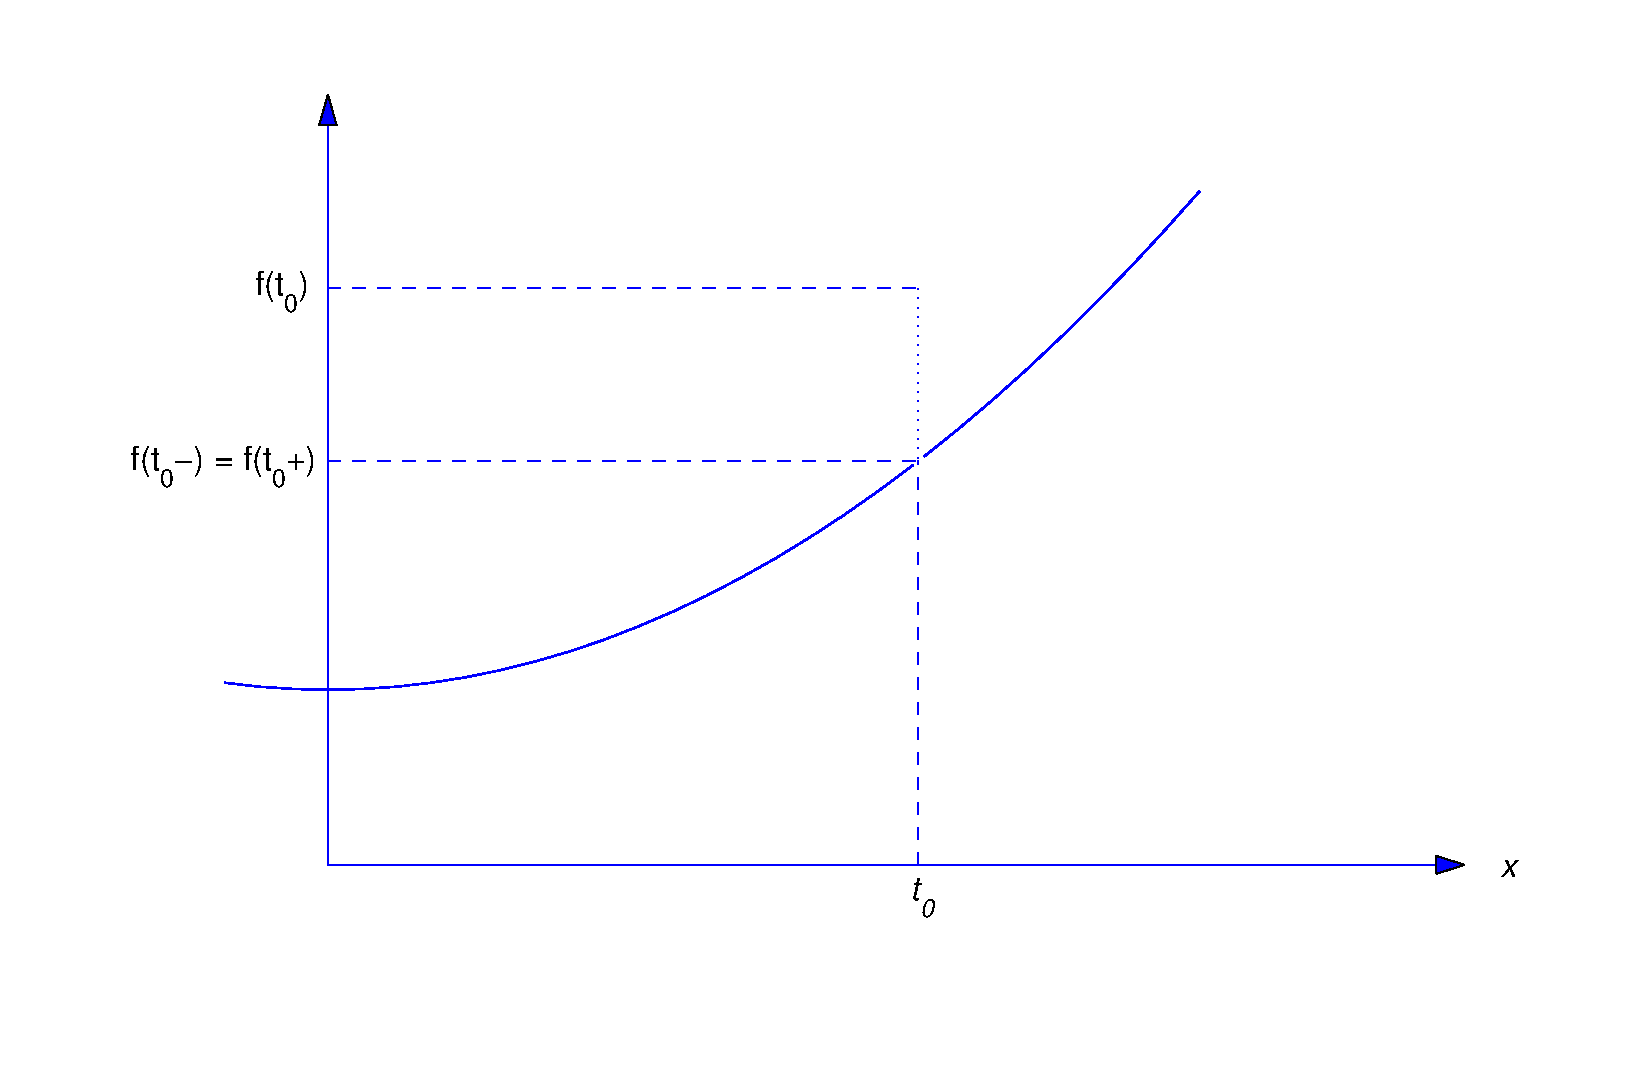
\includegraphics[bb=-78 148 689 643,width=5.67in,height=3.66in,keepaspectratio]{fig080102}}
  \caption{}
  \label{figure:8.1.2}
\end{minipage}
  \begin{minipage}[b]{0.5\linewidth}
    \centering
   \scalebox{.65}{
  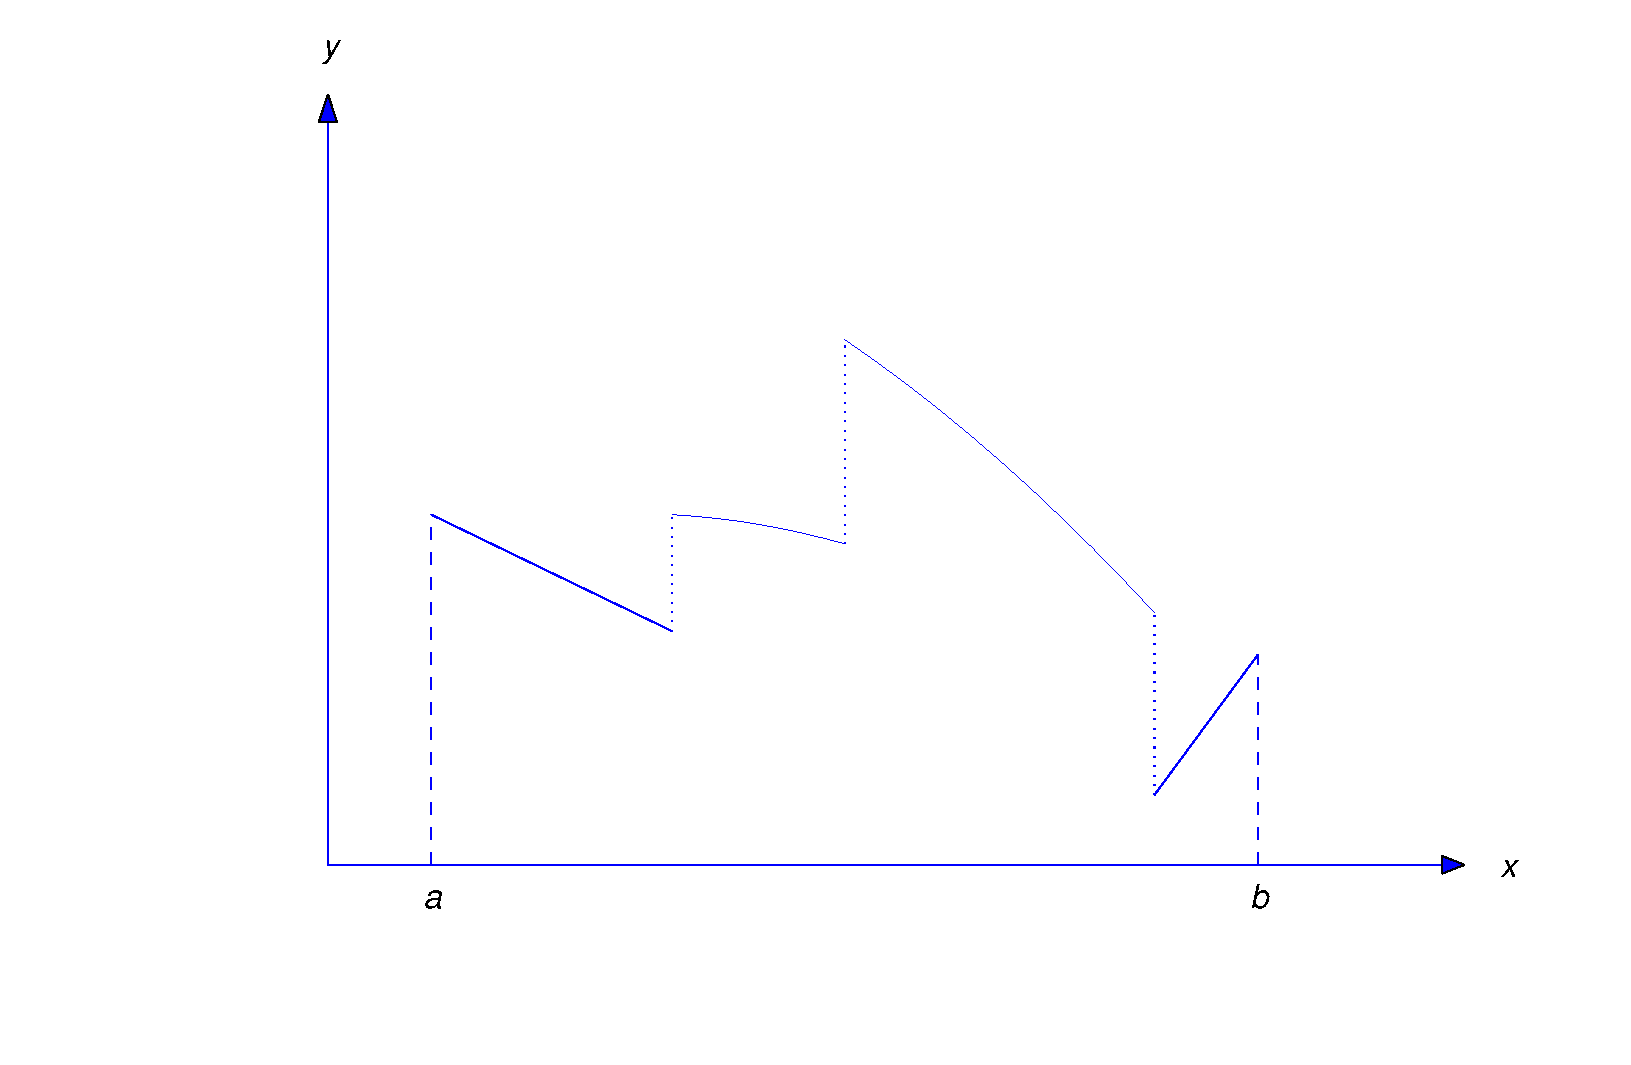
\includegraphics[bb=-78 148 689 643,width=5.67in,height=3.66in,keepaspectratio]{fig080103}}
\caption{A piecewise continuous function on $[a,b]$}
  \label{figure:8.1.3}
\end{minipage}
\end{figure}

\color{blue}
\remark{We know from calculus that a definite integral isn't
affected by changing the values of its integrand at isolated points.
Therefore, redefining a function $f$ to make it continuous at
removable discontinuities does not change ${\cal L}(f)$.}
\color{black}

\begin{definition}\color{blue}\label{thmtype:8.1.4}\rm
\mbox{}
\begin{rmlist}
\item % (i)
A function $f$ is said to be {\color{blue}\it piecewise continuous} on a finite
closed interval $[0,T]$ if $f(0+)$ and $f(T-)$ are finite and $f$ is
continuous on the open interval $(0,T)$ except possibly at finitely
many points, where $f$ may have jump discontinuities or removable
discontinuities.
\item % (ii)
A function $f$ is said to be {\color{blue}\it piecewise continuous} on the
infinite interval $[0,\infty)$ if it's piecewise continuous on
$[0,T]$ for every $T>0$.
\end{rmlist}
\end{definition}

Figure~\ref{figure:8.1.3} shows the graph of a typical piecewise
continuous function.

It is shown in calculus that if a function is piecewise continuous on
a finite closed interval then it's integrable on that interval. But
if $f$ is piecewise continuous on $[0,\infty)$, then so is $e^{-st}f
(t)$, and therefore
$$
\int_0^T e^{-st}f(t)\,dt
$$
exists for every $T>0$. However, piecewise continuity alone does not
guarantee that the improper integral
\begin{equation}\label{eq:8.1.13}
\int_0^\infty e^{-st}f(t)\,dt=\lim_{T\to\infty}\int_0^T e^{-st}f(t)\,
dt
\end{equation}
converges for $s$ in some interval $(s_0,\infty)$. For example, we
noted earlier that \eqref{eq:8.1.13} diverges for all $s$ if
$f(t)=e^{t^2}$. Stated informally, this occurs because $e^{t^2}$
increases too rapidly as $t\to\infty$. The next definition
provides a constraint on the growth of a function that guarantees
convergence of its Laplace transform for $s$ in some interval
$(s_0,\infty)$ .

\begin{definition}\color{blue}\label{thmtype:8.1.5}\rm A
function $f$ is said to be
{\color{blue}\it of exponential order\/} $s_0$ if there are constants $M$ and $t_0$
such that
\begin{equation}\label{eq:8.1.14}
|f(t)|\le Me^{s_0t},\quad t\ge t_0.
\end{equation}
In situations where the specific value of $s_0$
is irrelevant we say simply that $f$ is {\color{blue}\it of exponential order\/}.
\end{definition}

The next theorem gives useful sufficient conditions for a function $f$
to have a Laplace transform.  The proof is sketched in
Exercise~\ref{exer:8.1.10}.

\begin{theorem}\color{blue}\label{thmtype:8.1.6} If $f$
is piecewise continuous on $[0,\infty)$ and of exponential order $s_0$,
 then ${\cal L}(f)$ is defined for $s>s_0$.
\end{theorem}

\color{blue}
\remark{
We emphasize that the conditions of Theorem~\ref{thmtype:8.1.6}
 are sufficient, but {\color{blue}\it not necessary\/}, for $f$ to have a Laplace
transform. For example, Exercise~\ref{exer:8.1.14}\part{c} shows that  $f$
may have a Laplace transform even though $f$ isn't  of exponential
order.}
\color{black}

\begin{example}\label{example:8.1.8}\rm
If $f$ is bounded on some interval $[t_0,\infty)$, say
$$
|f(t)|\le M,\quad t\ge t_0,
$$
then \eqref{eq:8.1.14} holds with $s_0=0$, so $f$ is of exponential order
zero. Thus, for example, $\sin\omega t$ and $\cos \omega t$ are of
exponential order zero, and Theorem~\ref{thmtype:8.1.6} implies that
${\cal L}(\sin\omega t)$ and ${\cal L}(\cos \omega t)$ exist for
$s>0$. This is consistent with the conclusion of
Example~\ref{example:8.1.4}.
\end{example}

\begin{example}\label{example:8.1.9}\rm
It can be shown that if $\lim_{t\to\infty}e^{-s_0t}f(t)$ exists and is
finite then $f$ is of exponential order $s_0$
(Exercise~\ref{exer:8.1.9}). If $\alpha$ is any real number and $s_0>0$
then $f(t)=t^\alpha$ is of exponential order $s_0$, since
$$
\lim_{t\to\infty}e^{-s_0t}t^\alpha=0,
$$
by L'H\^opital's rule. If $\alpha\ge 0$, $f$ is also
continuous on $[0,\infty)$. Therefore Exercise~\ref{exer:8.1.9} and
Theorem~\ref{thmtype:8.1.6} imply that ${\cal L}(t^\alpha)$ exists for
$s\ge s_0$. However, since $s_0$ is an arbitrary positive number, this
really implies that ${\cal L}(t^\alpha)$ exists for all $s>0$. This is
consistent with the results of Example~\ref{example:8.1.2} and
Exercises~\ref{exer:8.1.6} and \ref{exer:8.1.8}.
\end{example}

\begin{example}\label{example:8.1.10}\rm
Find the Laplace transform of the piecewise continuous function
$$
f(t)=\left\{\begin{array}{cl} 1,&0\le t<1,\\  -3e^{-t},&t\ge
1.\end{array}\right.
$$
\end{example}

\solution    Since $f$ is defined by different formulas
on $[0,1)$ and $[1,\infty)$, we write
$$
 F(s)=\int_0^\infty e^{-st} f(t)\,dt
=\int_0^1e^{-st}(1)\,dt+\int_1^\infty
e^{-st}(-3e^{-t})\,dt.
$$
Since
$$
\int_0^1e^{-st}\,dt=\left\{\begin{array}{cl}\dst{{1-e^{-s}\over
s}},&\quad s\ne0,\\[2\jot] 1,&\quad s=0,\end{array}\right.
$$
 and
$$
\int_1^\infty e^{-st}(-3e^{-t})\,dt=-3\int_1^\infty
e^{-(s+1)t}\,dt=-{3e^{-(s+1)}\over s+1},\quad s>-1,
$$
it follows that
$$
F(s)=\left\{\begin{array}{rl}\dst{{1-e^{-s}\over
s}-3{e^{-(s+1)}\over
s+1}},&s>-1,\,s\ne0,\\\hfill\dst{1-{3\over e}}\hfill,&
s=0.\end{array}\right.
$$
This is consistent with Theorem~\ref{thmtype:8.1.6}, since
$$
|f(t)|\le 3e^{-t},\quad  t\ge 1,
$$
and therefore $f$ is of exponential order $s_0=-1$.

\color{blue}
\remark{In Section~8.4 we'll develop a more efficient
method for finding Laplace transforms of piecewise continuous
functions.}
\color{black}

\begin{example}\label{example:8.1.11}\rm
We stated  earlier that
$$
\int_0^\infty e^{-st} e^{t^2} dt=\infty
$$
for all $s$, so Theorem~\ref{thmtype:8.1.6} implies that $f(t)=e^{t^2}$
is not  of exponential order, since
$$
\lim_{t\to\infty} {e^{t^2}\over Me^{s_0t}}=\lim_{t\to\infty} {1\over
M} e^{t^2-s_0t}=\infty,
$$
so
$$
e^{t^2}>Me^{s_0t}
$$
for sufficiently large values of $t$, for any choice of $M$ and $s_{0}$
(Exercise~\ref{exer:8.1.3}).
\end{example}

\exercises

\begin{exerciselist}
\item\label{exer:8.1.1}
Find the Laplace transforms of the following functions by evaluating
the integral $F(s)=\int_0^\infty e^{-st} f(t)\,dt$.

\begin{tabular}[t]{@{}p{112pt}@{}p{112pt}@{}p{112pt}}
\part{a} $t$  & \part{b} $te^{-t}$ & \part{c} $\sinh bt$\\
 \part{d} $e^{2t}-3e^t$  & \part{e} $t^2$
\end{tabular}

\item\label{exer:8.1.2}
Use  the table of Laplace transforms to
find the Laplace transforms of the following functions.

\begin{tabular}[t]{@{}p{112pt}@{}p{112pt}@{}p{112pt}}
\part{a}  $\cosh t\sin t$ & \part{b}  $\sin^2t$ & \part{c}  $\cos^2
2t$\\ \part{d}  $\cosh^2 t$ & \part{e}  $t\sinh 2t$ & \part{f}
$\sin
t\cos t$\\ \part{g}  $\dst{\sin\left(t+{\pi\over
4}\right)}$ & \part{h}  $\cos 2t -\cos 3t$ & \part{i}  $\sin 2t +\cos
4t$
\end{tabular}

\item\label{exer:8.1.3}
 Show that
$$
\int_0^\infty e^{-st}e^{t^2} dt=\infty
$$
for every real number $s$.

\item\label{exer:8.1.4}
 Graph the following piecewise continuous functions and evaluate
$f(t+)$, $f(t-)$, and $f(t)$ at each point of discontinuity.

\begin{tabular}[t]{@{}p{168pt}@{}p{168pt}}
\part{a} $f(t)=\left\{\begin{array}{cl} -t,
& 0\le t<2,\\ t-4, & 2\le t<3,\\ 1, & t\ge
3.\end{array}\right.$ &
\part{b} $f(t)=\left\{\begin{array}{cl} t^2+2, & 0
\le t<1,\\4, & t=1,\\ t, & t>
1.\end{array}\right.$\\[15pt]
\part{c} $f(t)=\left\{\begin{array}{rl}
\sin t, & 0\le t<\pi/ 2,\\ 2\sin t, &\pi/ 2
\le t<\pi,\\ \cos t, & t\ge\pi.\end{array}\right.$ &
\part{d} $f(t)=\left\{\begin{array}{cl}t,
 & 0\le t<1,\\ 2, & t=1,\\ 2-t, & 1
\le t<2,\\ 3, & t=2,\\ 6, & t>
2.\end{array}\right.$
\end{tabular}

\item\label{exer:8.1.5}
 Find the Laplace transform:

\begin{tabular}[t]{@{}p{168pt}@{}p{168pt}}
\part{a} $f(t)=\left\{\begin{array}{rl} e^{-t}, &
0\le t<1,\\ e^{-2t}, & t\ge 1.\end{array}\right.$ &
\part{b} $f(t)=\left\{\begin{array}{rl} 1, & 0\le t<
4,\\ t, & t\ge 4.\end{array}\right.$\\[2\jot]
\part{c} $f(t)=\left\{\begin{array}{rl} t, & 0\le
t<1,\\ 1, & t\ge 1.\end{array}\right.$&
\part{d}  $f(t)=\left\{\begin{array}{rl} te^t, & 0\le
t<1,\\\phantom{t} e^t, & t\ge 1.\end{array}\right.$
\end{tabular}

\item\label{exer:8.1.6}
Prove that if $f(t)\leftrightarrow F(s)$ then $t^kf(t)\leftrightarrow
(-1)^kF^{(k)}(s)$. \hint{Assume that it's permissible to differentiate
the integral $\int_0^\infty e^{-st}f(t)\,dt$ with respect to $s$ under
the integral sign.}

\item\label{exer:8.1.7}
Use the known Laplace transforms
$$
{\cal L}(e^{\lambda t}\sin\omega t)={\omega\over(s-\lambda)^2+\omega^2}
\quad\mbox{and }\quad
{\cal L}(e^{\lambda t}\cos\omega t)={s-\lambda\over(s-\lambda)^2+\omega^2}
$$
  and the result of Exercise~\ref{exer:8.1.6} to find
${\cal L}(te^{\lambda t}\cos\omega t)$ and
${\cal L}(te^{\lambda t}\sin\omega t)$.

\item\label{exer:8.1.8}
 Use the known Laplace transform ${\cal L}(1)=1/s$ and the result of
Exercise~\ref{exer:8.1.6} to show that
$$
{\cal L}(t^n)={n!\over s^{n+1}},\quad n=\mbox{ integer}.
$$

\item\label{exer:8.1.9}
\begin{alist}
\item % (a)
 Show that if $\lim_{t\to\infty} e^{-s_0t} f(t)$ exists and
is finite then  $f$ is of exponential order $s_0$.
\item % (b)
 Show that if $f$ is of exponential order $s_0$ then $\lim_{t
\to\infty} e^{-st} f(t)=0$ for all $s>s_0$.
\item % (c)
Show that if $f$ is of exponential order $s_0$  and $g(t)=f(t+\tau)$
where $\tau>0$, then $g$ is also of exponential order $s_0$.
\end{alist}

\item\label{exer:8.1.10}
Recall the next  theorem from calculus.

\color{blue}
{\sc Theorem A.} \it Let $g$ be integrable on $[0,T]$ for
every $T>0$.  Suppose there's a function $w$ defined on some
interval $[\tau,\infty)$ (with $\tau\ge 0$) such that $|g(t)|\le
w(t)$ for $t\ge\tau$ and $\int^\infty_\tau w(t)\,dt$
converges.  Then $\int_0^\infty g(t)\,dt$ converges.\rm
\color{black}

Use Theorem A to show that if $f$ is piecewise continuous on
$[0,\infty)$ and of exponential order $s_0$, then $f$ has a Laplace
transform $F(s)$ defined for $s>s_0$.

\item\label{exer:8.1.11}
 Prove: If $f$ is piecewise continuous and of exponential order
then $\lim_{s\to\infty}F(s)~=~0$.

\item\label{exer:8.1.12}
Prove: If $f$ is continuous on $[0,\infty)$ and of exponential order
$s_0>0$, then
$$
{\cal L}\left(\int^t_0 f(\tau)\,d\tau\right)={1\over s} {\cal L} (f),
\quad s>s_0.
$$
\hint{Use integration by parts to evaluate the transform on
the left.}

\item\label{exer:8.1.13}
Suppose $f$ is piecewise continuous and of exponential
order, and that $\lim_{t\to 0+} f(t)/t$ exists.  Show that
$$
{\cal L}\left({f(t)\over t}\right)=\int^\infty_s F(r)\,dr.
$$
\hint{Use  the results of Exercises~$6$ and $11$.}

\item\label{exer:8.1.14}
Suppose $f$ is piecewise continuous on $[0,\infty)$.
\begin{alist}
\item % (a)
Prove: If the integral $g(t)=\int^t_0 e^{-s_0\tau} f(\tau)\,d\tau$
satisfies the inequality $|g(t)|\le M\; (t\ge 0)$, then $f$ has a
Laplace transform $F(s)$ defined for $s>s_0$. \hint{Use integration by
parts to show that
$$
\int_0^T e^{-st}f(t)\,dt = e^{-(s-s_0)T}g(T)
+(s-s_0)\int_0^Te^{-(s-s_0)t}g(t)\,dt.
$$}
\item % (b)
 Show that if ${\cal L}(f)$ exists for
$s=s_0$ then it exists for $s>s_0$.
Show that the function
$$
f(t)=te^{t^2}\cos(e^{t^2})
$$
has a Laplace transform defined for $s>0$, even though $f$ isn't  of
exponential order.
\item % (c)
Show that the function
$$
f(t)=te^{t^2}\cos(e^{t^2})
$$
has a Laplace transform defined for $s>0$, even though $f$ isn't  of
exponential order.
\end{alist}

\item\label{exer:8.1.15}
Use the table of Laplace transforms and the result of
Exercise~\ref{exer:8.1.13} to find the Laplace transforms of the following
functions.

\begin{tabular}[t]{@{}p{112pt}@{}p{112pt}@{}p{112pt}}
\part{a} $\dst{{\sin\omega t\over t}\quad(\omega>0)}$ &
\part{b} $\dst{{\cos\omega t-1\over t}}\quad (\omega>0)$ &
\part{c} $\dst{{e^{at}-e^{bt}\over t}}$\\[2\jot]
\part{d} $\dst{{\cosh t-1\over t}}$ &
\part{e} $\dst{{\sinh^2 t\over t}}$
\end{tabular}

\item\label{exer:8.1.16}
  The {\color{blue}\it gamma function} is defined by
$$
\Gamma (\alpha)=\int_0^\infty x^{\alpha-1}e^{-x}\,dx,
$$
which can be shown to converge if $\alpha>0$.
\begin{alist}
\item % (a)
 Use integration by parts to show that
$$
\Gamma (\alpha+1)=\alpha\Gamma (\alpha),\quad\alpha>0.
$$
\item % (b)
 Show that $\Gamma(n+1)=n!$ if $n=1$, $2$, $3$,\dots.
\item % (c)
 From  \part{b} and the table of Laplace transforms,
$$
{\cal L}(t^\alpha)={\Gamma (\alpha+1)\over s^{\alpha+1}},\quad s>0,
$$
if $\alpha$ is a nonnegative integer.  Show that this formula is valid for
any $\alpha>-1$. \hint{Change the variable of integration in the
integral for $\Gamma (\alpha+1)$.}
\end{alist}

\item\label{exer:8.1.17}
  Suppose $f$ is continuous on $[0, T]$ and $f(t+T)=f(t)$
for all $t\ge 0$.  (We say in this case that $f$ is {\color{blue}\it periodic with
period\/} $T$.)
\begin{alist}
\item % (a)
 Conclude from Theorem~\ref{thmtype:8.1.6} that the Laplace transform of
$f$ is defined for $s>0$. \hint{Since $f$ is
continuous on $[0,T]$ and periodic with period $T$, it's bounded
on $[0,\infty)$.}
\item % (b)
 \part{b} Show that
$$
F(s)={1\over 1-e^{-sT}}\int_0^T e^{-st}f(t)\,dt,\quad s>0.
$$
\hint{Write
$$
F(s)=\sum^\infty_{n=0}\int^{(n+1)T}_{nT}e^{-st} f(t)\,dt.
$$
Then show that
$$
\int^{(n+1)T}_{nT} e^{-st}f(t)\,dt=e^{-nsT}\int_0^T e^{-st}f(t)\,dt,
$$
and recall the formula for the sum of a geometric series.}
\end{alist}

\item\label{exer:8.1.18}
  Use the formula given in Exercise~\ref{exer:8.1.17}\part{b} to find
the
Laplace transforms of the given periodic functions:
\begin{alist}
\item % (a)
 $\dst{f(t)=\left\{\begin{array}{cl} t, & 0\le
t<1,\\ 2-t, & 1\le t<2,\end{array}\right.\hskip30pt f(t+2)=f(t),
\quad t\ge 0}$
\item % (b)
 $\dst{f(t)=\left\{\begin{array}{rl}1, & 0\le
t<{1\over 2},\\ -1, & {1\over 2}\le t<1,\end{array}\right.
\hskip30pt f(t+1)=f(t),\quad t\ge 0}$
\item % (c)
 $f(t)=|\sin t|$
\item % (d)
 $\dst{f(t)=\left\{\begin{array}{cl}\sin t, & 0\le t<
\pi,
\\ 0, &\pi\le t<2\pi,\end{array}\right.\hskip30pt
f(t+2\pi)=f(t)}$
\end{alist}

\end{exerciselist}


\section{The Inverse Laplace Transform}

\noindent
\boxit{Definition of the Inverse Laplace Transform}

\noindent
In Section~8.1 we defined the Laplace transform
of
$f$ by
$$
F(s)={\cal L}(f)=\int_0^\infty e^{-st}f(t)\,dt.
$$
We'll also say that $f$ is an {\color{blue}\it inverse Laplace Transform\/} of
$F$, and write
$$
f={\cal L}^{-1}(F).
$$
To solve differential equations with the Laplace transform, we
must be able to obtain $f$ from its transform $F$. There's a formula
for doing this, but we can't use it because it requires the theory of
functions of a complex variable. Fortunately, we can use the table of
Laplace transforms to find inverse transforms that we'll need.

\begin{example}\label{example:8.2.1}\rm Use the table of Laplace
transforms to find
$$
\mbox{\part{a} }{\cal L}^{-1}\left({1\over s^2-1}\right)
\mbox{\quad and \quad\part{b} }{\cal L}^{-1}\left({s\over
s^2+9}\right).
$$
\end{example}

\solutionpart{a}
Setting $b=1$ in  the transform pair
$$
\sinh bt\leftrightarrow {b\over s^2-b^2}
$$
shows that
$$
{\cal L}^{-1}\left({1\over s^2-1}\right)=\sinh t.
$$

\solutionpart{b}
Setting $\omega=3$ in  the transform pair
$$
\cos\omega t\leftrightarrow{s\over s^2+\omega^2}
$$
shows that
$$
{\cal L}^{-1}\left({s\over s^2+9}\right)=\cos3t.\bbox
$$

The next theorem enables us to find inverse transforms of linear
combinations of transforms in the table. We omit the proof.

\begin{theorem}\color{blue}$[$Linearity Property$]$\label{thmtype:8.2.1}
If $F_1,$ $F_2,$ \dots$,$ $F_n$ are Laplace transforms and
$c_1,$ $c_2,$ \dots, $c_n$ are constants$,$ then
$$
{\cal L}^{-1}(c_1F_1+c_2F_2+\cdots+c_nF_n)=c_1{\cal L}^{-1}(F_1)+c_2{\cal
L}^{-1}(F_2)+\cdots+c_n{\cal L}^{-1}F_n.
$$
\end{theorem}

\begin{example}\label{example:8.2.2}\rm Find
$$
{\cal L}^{-1}\left({8\over s+5}+{7\over s^2+3}\right).
$$
\end{example}

\solution
From the table of Laplace transforms in Section~8.8,,
$$
e^{at}\leftrightarrow {1\over s-a}\quad\mbox{ and }\quad
\sin\omega t\leftrightarrow {\omega\over s^2+\omega^2}.
$$
Theorem~\ref{thmtype:8.2.1}
with $a=-5$ and   $\omega=\sqrt3$
yields
\begin{eqnarray*}
{\cal L}^{-1}\left({8\over s+5}+{7\over s^2+3}\right)&=&
8{\cal L}^{-1}\left({1\over s+5}\right)+7{\cal L}^{-1}\left({1\over
s^2+3}\right)\\[10pt]
&=&
8{\cal L}^{-1}\left({1\over s+5}\right)+{7\over\sqrt3}{\cal
L}^{-1}\left({\sqrt3\over
s^2+3}\right)\\[10pt]&=&8e^{-5t}+{7\over\sqrt3}\sin\sqrt3t.
\end{eqnarray*}

\begin{example}\label{example:8.2.3}\rm Find
$$
{\cal L}^{-1}\left({3s+8\over s^2+2s+5}\right).
$$
\end{example}

\solution
Completing the square in the denominator yields
$$
{3s+8\over s^2+2s+5}={3s+8\over(s+1)^2+4}.
$$
Because of the form of the denominator, we consider
the transform pairs
$$
 e^{-t}\cos 2t\leftrightarrow{s+1\over(s+1)^2+4}
\mbox{\quad and \quad}
 e^{-t}\sin 2t\leftrightarrow{2\over(s+1)^2+4},
$$
and write
\begin{eqnarray*}
{\cal L}^{-1}\left({3s+8\over(s+1)^2+4}\right)&=&
{\cal L}^{-1}\left({3s+3\over(s+1)^2+4}\right)+
{\cal L}^{-1}\left({5\over(s+1)^2+4}\right)\\[10pt]&=&
3{\cal L}^{-1}\left({s+1\over(s+1)^2+4}\right)+
{5\over2}{\cal L}^{-1}\left({2\over(s+1)^2+4}\right)\\[10pt]&=&
e^{-t}(3\cos 2t+{5\over2}\sin 2t).
\end{eqnarray*}

\color{blue}
\remark{We'll often write inverse Laplace transforms of specific
functions without explicitly stating how they are obtained. In such
cases you should refer to the table of Laplace transforms in Section~8.8.}
\color{black}

\boxit{Inverse Laplace Transforms of Rational Functions}

\noindent
Using the Laplace transform to
 solve differential equations
often requires  finding the inverse
transform of a rational function
$$
F(s)={P(s)\over Q(s)},
$$
where $P$ and $Q$ are polynomials in $s$ with no common factors. Since
it can be shown that $\lim_{s\to\infty}F(s)=0$ if $F$ is a Laplace
transform, we need only consider the case where
$\mbox{degree}(P)<\mbox{degree}(Q)$. To obtain ${\cal L}^{-1}(F)$, we
find the partial fraction expansion of $F$, obtain inverse transforms
of the individual terms in the expansion from the table of Laplace
transforms, and use the linearity property of the inverse transform.
The next two examples illustrate this.

\begin{example}\label{example:8.2.4}\rm Find the inverse Laplace transform
of
\begin{equation}\label{eq:8.2.1}
F(s)={3s+2\over s^2-3s+2}.
\end{equation}
\end{example}

\solution ({\sc Method 1})
 Factoring the denominator in  \eqref{eq:8.2.1} yields
\begin{equation}\label{eq:8.2.2}
F(s)={3s+2\over(s-1)(s-2)}.
\end{equation}
The form for the partial fraction expansion is
\begin{equation}\label{eq:8.2.3}
{3s+2\over(s-1)(s-2)}={A\over s-1}+{B\over s-2}.
\end{equation}
Multiplying  this by $(s-1)(s-2)$ yields
$$
3s+2=(s-2)A+(s-1)B.
$$
Setting $s=2$ yields $B=8$ and setting $s=1$ yields $A=-5$. Therefore
$$
F(s)=-{5\over s-1}+{8\over s-2}
$$
and
$$
{\cal L}^{-1}(F)=-5{\cal L}^{-1}\left({1\over s-1}\right)
+8{\cal L}^{-1}\left({1\over s-2}\right)=-5e^t+8e^{2t}.
$$

\solution ({\sc Method 2})
We don't really have to multiply  \eqref{eq:8.2.3} by $(s-1)(s-2)$
to compute $A$ and $B$. We can obtain $A$ by simply ignoring the factor
$s-1$ in the denominator of  \eqref{eq:8.2.2} and setting $s=1$ elsewhere;
thus,
\begin{equation}\label{eq:8.2.4}
A=\left.{3s+2\over s-2}\right|_{s=1}={3\cdot1+2\over 1-2}=-5.
\end{equation}
Similarly, we can obtain $B$ by ignoring the factor
$s-2$ in the denominator of  \eqref{eq:8.2.2} and setting $s=2$ elsewhere;
thus,
\begin{equation}\label{eq:8.2.5}
B=\left.{3s+2\over s-1}\right|_{s=2}={3\cdot2+2\over2-1}=8.
\end{equation}
To justify this, we observe that multiplying  \eqref{eq:8.2.3} by $s-1$
yields
$$
{3s+2\over s-2}=A+(s-1){B\over s-2},
$$
and setting $s=1$ leads to
\eqref{eq:8.2.4}. Similarly, multiplying  \eqref{eq:8.2.3} by $s-2$ yields
$$
{3s+2\over s-1}=(s-2){A\over s-2}+B
$$
and setting $s=2$ leads to
\eqref{eq:8.2.5}.  (It isn't necesary to
 write the last two equations. We wrote them  only to justify
the shortcut procedure indicated in  \eqref{eq:8.2.4} and
\eqref{eq:8.2.5}.) \bbox

The shortcut employed in the second solution of
Example~\ref{example:8.2.4} is
\href{https://mathshistory.st-andrews.ac.uk/Biographies/Heaviside/}
 {\color{blue}\it Heaviside's method}.
The next theorem states this method formally. For a proof
and an extension of this theorem, see Exercise~\ref{exer:8.2.10}.

\begin{theorem}\color{blue}\label{thmtype:8.2.2}
Suppose
\begin{equation}\label{eq:8.2.6}
F(s)={P(s)\over(s-s_1)(s-s_2)\cdots(s-s_n)},
\end{equation}
where $s_1$, $s_2,$ \dots$,$ $s_n$ are distinct  and $P$ is a polynomial of
degree less than $n.$  Then
$$
F(s)={A_1\over s-s_1}+{A_2\over s-s_2}+\cdots+{A_n\over s-s_n},$$
where $A_i$ can be computed from \eqref{eq:8.2.6}
by ignoring the factor $s-s_i$  and setting $s=s_i$ elsewhere.
\end{theorem}

\begin{example}\label{example:8.2.5}\rm Find the inverse Laplace transform
of
\begin{equation}\label{eq:8.2.7}
F(s)={6+(s+1)(s^2-5s+11)\over s(s-1)(s-2)(s+1)}.
\end{equation}
\end{example}

\solution
The partial fraction expansion of  \eqref{eq:8.2.7} is of the form
\begin{equation}\label{eq:8.2.8}
F(s)={A\over s}+{B\over s-1}+{C\over s-2}+{D\over s+1}.
\end{equation}
To find $A$, we ignore the factor $s$ in the denominator of
\eqref{eq:8.2.7} and set $s=0$ elsewhere. This yields
$$
A={6+(1)(11)\over(-1)(-2)(1)}={17\over2}.
$$
Similarly, the other coefficients are given by
$$
B={6+(2)(7)\over(1)(-1)(2)}=-10,
$$
$$
C={6+3(5)\over2(1)(3)}={7\over2},
$$
and
$$
D={6\over(-1)(-2)(-3)}=-1.
$$
Therefore
$$
F(s)={17\over2}\,{1\over s}-{10\over s-1}+{7\over2}\,{1\over
s-2}-{1\over s+1}
$$
and
\begin{eqnarray*}
{\cal L}^{-1}(F)&=&
 {17\over2}{\cal L}^{-1}\left(1\over s\right)-10{\cal L}^{-1}\left(1
\over s-1\right)+{7\over
2}{\cal L}^{-1}\left(1\over s-2\right)-{\cal L}^{-1}\left(1\over
s+1\right)\\[1\jot]
&=& {17\over2}-10e^t+{7\over2}e^{2t}-e^{-t}.
\end{eqnarray*}

\color{blue}
\remark{We didn't ``multiply out'' the numerator in
\eqref{eq:8.2.7} before
computing the coefficients in \eqref{eq:8.2.8}, since
 it wouldn't simplify the computations.}
\color{black}

\begin{example}\label{example:8.2.6}\rm Find the inverse Laplace transform
of
\begin{equation}\label{eq:8.2.9}
F(s)={8-(s+2)(4s+10)\over(s+1)(s+2)^2}.
\end{equation}
\end{example}

\solution
The  form for the partial fraction expansion  is
\begin{equation}\label{eq:8.2.10}
F(s)={A\over s+1}+{B\over s+2}+{C\over(s+2)^2}.
\end{equation}
Because of the repeated factor $(s+2)^2$ in \eqref{eq:8.2.9}, Heaviside's
method doesn't work. Instead, we find a common denominator in
\eqref{eq:8.2.10}. This yields
\begin{equation}\label{eq:8.2.11}
F(s)={A(s+2)^2+B(s+1)(s+2)+C(s+1)\over(s+1)(s+2)^2}.
\end{equation}
If  \eqref{eq:8.2.9} and  \eqref{eq:8.2.11} are to be equivalent, then
\begin{equation}\label{eq:8.2.12}
A(s+2)^2+B(s+1)(s+2)+C(s+1)=8-(s+2)(4s+10).
\end{equation}
The two sides of this equation are polynomials of degree two. From a
theorem of algebra, they will be equal for all $s$ if they are equal
for any three distinct values of $s$. We may determine $A$, $B$ and
$C$ by choosing convenient values of $s$.

The left side of \eqref{eq:8.2.12} suggests that we take $s=-2$ to obtain
$C=-8$, and $s=-1$ to obtain $A=2$. We can now choose any third value
of $s$ to determine $B$. Taking $s=0$ yields $4A+2B+C=-12$. Since
$A=2$ and $C=-8$ this implies that $B=-6$. Therefore
$$
F(s)={2\over s+1}-{6\over s+2}-{8\over(s+2)^2}
$$
and
\begin{eqnarray*}
{\cal L}^{-1}(F)&=&
2{\cal L}^{-1}\left(1\over s+1\right)-6{\cal L}^{-1}\left(1\over
s+2\right)-8{\cal L}^{-1}\left(1\over(s+2)^2\right)\\[1\jot]
&=&2e^{-t}-6e^{-2t}-8te^{-2t}.
\end{eqnarray*}

\begin{example}\label{example:8.2.7}\rm Find the inverse Laplace transform
of
$$
F(s)={s^2-5s+7\over(s+2)^3}.
$$
\end{example}

\solution
The form for the partial fraction expansion  is
$$
F(s)={A\over s+2}+{B\over(s+2)^2}+{C\over(s+2)^3}.
$$
The easiest way to obtain $A$, $B$, and $C$ is to expand the numerator
in powers of $s+2$. This yields
$$
s^2-5s+7=[(s+2)-2]^2-5[(s+2)-2]+7=(s+2)^2-9(s+2)+21.
$$
Therefore
\begin{eqnarray*}
F(s)&=&{(s+2)^2-9(s+2)+21\over(s+2)^3}\\[10pt]
&=&{1\over s+2}-{9\over(s+2)^2}+{21\over(s+2)^3}
\end{eqnarray*}
and
\begin{eqnarray*}
{\cal L}^{-1}(F)&=&
{\cal L}^{-1}\left({1\over s+2}\right)-9{\cal
L}^{-1}\left({1\over(s+2)^2}\right)+{21\over2}{\cal
L}^{-1}\left({2\over(s+2)^3}\right)\\[10pt]&=&
e^{-2t}\left(1-9t+{21\over2}t^2\right).
\end{eqnarray*}

\begin{example}\label{example:8.2.8}\rm %\exampleinverse
 Find the inverse Laplace transform of
\begin{equation}\label{eq:8.2.13}
F(s)={1-s(5+3s)\over s\left[(s+1)^2+1\right]}.
\end{equation}
\end{example}

\solution
One  form for the partial fraction expansion of $F$ is
\begin{equation}\label{eq:8.2.14}
F(s)={A\over s}+{Bs+C\over(s+1)^2+1}.
\end{equation}
However, we see from the table of Laplace transforms that the inverse
transform of the second fraction on the right of \eqref{eq:8.2.14} will be
a linear combination of the inverse transforms
$$
e^{-t}\cos t\quad\mbox{ and }\quad e^{-t}\sin t
$$
of
$$
{s+1\over(s+1)^2+1}\quad\mbox{ and }\quad {1\over(s+1)^2+1}
$$
respectively. Therefore, instead of \eqref{eq:8.2.14} we write
\begin{equation}\label{eq:8.2.15}
F(s)={A\over s}+{B(s+1)+C\over(s+1)^2+1}.
\end{equation}
Finding a common denominator yields
\begin{equation}\label{eq:8.2.16}
F(s)={A\left[(s+1)^2+1\right]+B(s+1)s+Cs\over
s\left[(s+1)^2+1\right]}.
\end{equation}
If  \eqref{eq:8.2.13} and  \eqref{eq:8.2.16} are to be equivalent, then
$$
A\left[(s+1)^2+1\right]+B(s+1)s+Cs=1-s(5+3s).
$$
This is true for all $s$ if it's true for three distinct values of
$s$.  Choosing $s=0$, $-1$, and $1$ yields the system
$$
\begin{array}{rcr}
2A&=&1\phantom{.}\\ A-C&=&3\phantom{.}\\5A+2B+C&=&-7.
\end{array}
$$
Solving this system yields
$$
A={1\over2},\quad B=-{7\over2},\quad C=-{5\over2}.
$$
Hence, from  \eqref{eq:8.2.15},
$$
F(s)={1\over2s}-{7\over2}\,{s+1\over(s+1)^2+1}-
{5\over2}\,{1\over(s+1)^2+1}.
$$
Therefore
\begin{eqnarray*}
{\cal L}^{-1}(F)&=&
{1\over2}{\cal L}^{-1}\left(1\over s\right)-{7\over2}{\cal
L}^{-1}\left(s+1
\over(s+1)^2+1\right)-{5\over2} {\cal L}^{-1}\left(1\over
(s+1)^2+1\right)\\[1\jot]
&=& {1\over2}-{7\over2}e^{-t}\cos t-{5\over2}e^{-t}\sin t.
\end{eqnarray*}

\begin{example}\label{example:8.2.9}\rm Find the inverse Laplace transform of
\begin{equation}\label{eq:8.2.17}
F(s)={8+3s\over(s^2+1)(s^2+4)}.
\end{equation}
\end{example}

\solution
The form for the partial fraction expansion is
$$
F(s)={A+Bs\over s^2+1}+{C+Ds\over s^2+4}.
$$
The coefficients $A$, $B$, $C$ and $D$ can be obtained by finding a common
denominator and equating the resulting numerator to the numerator in
\eqref{eq:8.2.17}. However, since there's no first power of $s$ in the
denominator of \eqref{eq:8.2.17}, there's an easier way: the expansion of
$$
F_1(s)={1\over(s^2+1)(s^2+4)}
$$
can be obtained quickly by using Heaviside's method to expand
$$
{1\over(x+1)(x+4)}={1\over3}\left({1\over x+1}-{1\over x+4}\right)
$$
and then setting $x=s^2$ to obtain
$$
{1\over(s^2+1)(s^2+4)}={1\over3}\left({1\over s^2+1}-{1\over
s^2+4}\right).
$$
Multiplying this by $8+3s$ yields
$$
F(s)={8+3s\over(s^2+1)(s^2+4)}={1\over3}\left({8+3s\over s^2+1}-{8+3s\over
s^2+4}\right).
$$
Therefore
$$
{\cal L}^{-1}(F)={8\over3}\sin t+\cos t-{4\over3}\sin 2t-\cos 2t.
$$

\technology

\medskip

Some software packages that do symbolic algebra can find partial
fraction expansions very easily. We recommend that you use such a
package if one is available to you, but only after you've  done
enough partial fraction expansions on your own to  master the
technique.

\exercises

\begin{exerciselist}
\item\label{exer:8.2.1}
 Use the table of Laplace transforms  to find the inverse Laplace
transform.

\begin{tabular}[t]{@{}p{112pt}@{}p{112pt}@{}p{112pt}}
\part{a} $\dst{3\over(s-7)^4}$ &
\part{b} $\dst{2s-4\over s^2-4s+13}$ &
\part{c} $\dst{1\over s^2+4s+20}$\\[10pt]
\part{d} $\dst{2\over s^2+9}$ &
\part{e} $\dst{s^2-1\over(s^2+1)^2}$ &
\part{f} $\dst{1\over(s-2)^2-4}$\\[10pt]
\part{g} $\dst{12s-24\over(s^2-4s+85)^2}$ &
\part{h} $\dst{2\over(s-3)^2-9}$ &
\part{i} $\dst{s^2-4s+3\over(s^2-4s+5)^2}$
\end{tabular}

\item\label{exer:8.2.2}
 Use Theorem~\ref{thmtype:8.2.1} and the table of Laplace transforms
  to find the inverse Laplace transform.

\begin{tabular}[t]{@{}p{112pt}@{}p{112pt}@{}p{112pt}}
\part{a}  $\dst{2s+3\over(s-7)^4}$ &
\part{b}  $\dst{s^2-1\over(s-2)^6}$ &
\part{c}  $\dst{s+5\over s^2+6s+18}$\\[10pt]
\part{d}  $\dst{2s+1\over s^2+9}$ &
\part{e}  $\dst{s\over s^2+2s+1}$ &
\part{f}  $\dst{s+1\over s^2-9}$\\[10pt]
\part{g}  $\dst{s^3+2s^2-s-3\over(s+1)^4}$ &
\part{h}  $\dst{2s+3\over(s-1)^2+4}$ &
\part{i}  $\dst{1\over s}-{s\over s^2+1}$\\[10pt]
\part{j}  $\dst{3s+4\over s^2-1}$ &
\part{k}  $\dst{3\over s-1}+{4s+1\over s^2+9}$ &
\part{l}  $\dst{3\over(s+2)^2}-{2s+6\over s^2+4}$
\end{tabular}

\item\label{exer:8.2.3}
 Use Heaviside's method to find the inverse Laplace transform.

\begin{tabular}[t]{@{}p{168pt}@{}p{168pt}}
\part{a}  $\dst{3-(s+1)(s-2)\over(s+1)(s+2)(s-2)}$&
\part{b}  $\dst{7+(s+4)(18-3s)\over(s-3)(s-1)(s+4)}$\\[10pt]
\part{c}  $\dst{2+(s-2)(3-2s)\over(s-2)(s+2)(s-3)}$ &
\part{d}  $\dst{3-(s-1)(s+1)\over(s+4)(s-2)(s-1)}$\\[10pt]
\part{e}
$\dst{3+(s-2)(10-2s-s^2)\over(s-2)(s+2)(s-1)(s+3)}$
&
\part{f}  $\dst{3+(s-3)(2s^2+s-21)\over(s-3)(s-1)(s+4)(s-2)}$
\end{tabular}

\item\label{exer:8.2.4}
 Find the inverse Laplace transform.

\begin{tabular}[t]{@{}p{168pt}@{}p{168pt}}
\part{a}  $\dst{2+3s\over(s^2+1)(s+2)(s+1)}$&
\part{b}  $\dst{3s^2+2s+1\over(s^2+1)(s^2+2s+2)}$\\[10pt]
\part{c}  $\dst{3s+2\over(s-2)(s^2+2s+5)}$ &
\part{d}  $\dst{3s^2+2s+1\over(s-1)^2(s+2)(s+3)}$\\[10pt]
\part{e}  $\dst{2s^2+s+3\over(s-1)^2(s+2)^2}$ &
\part{f}  $\dst{3s+2\over(s^2+1)(s-1)^2}$
\end{tabular}

\item\label{exer:8.2.5}
 Use the method of Example~\ref{example:8.2.9}  to find the
inverse Laplace transform.

\begin{tabular}[t]{@{}p{112pt}@{}p{112pt}@{}p{112pt}}
\part{a} $\dst{3s+2\over(s^2+4)(s^2+9)}$ &
\part{b} $\dst{-4s+1\over(s^2+1)(s^2+16)}$ &
\part{c} $\dst{5s+3\over(s^2+1)(s^2+4)}$\\[10pt]
\part{d} $\dst{-s+1\over(4s^2+1)(s^2+1)}$ &
\part{e} $\dst{17s-34\over(s^2+16)(16s^2+1)}$ &
\part{f} $\dst{2s-1\over(4s^2+1)(9s^2+1)}$
\end{tabular}

\item\label{exer:8.2.6}
 Find the inverse Laplace transform.

\begin{tabular}[t]{@{}p{168pt}@{}p{168pt}}
\part{a} $\dst{17 s-15\over(s^2-2s+5)(s^2+2s+10)}$ &
\part{b} $\dst{8s+56\over(s^2-6s+13)(s^2+2s+5)}$\\[10pt]
\part{c} $\dst{s+9\over(s^2+4s+5)(s^2-4s+13)}$ &
\part{d} $\dst{3s-2\over(s^2-4s+5)(s^2-6s+13)}$\\[10pt]
\part{e} $\dst{3s-1\over(s^2-2s+2)(s^2+2s+5)}$ &
\part{f} $\dst{20s+40\over(4s^2-4s+5)(4s^2+4s+5)}$
\end{tabular}

\item\label{exer:8.2.7}
Find the inverse Laplace transform.

\begin{tabular}[t]{@{}p{168pt}@{}p{168pt}}
 \part{a} $\dst{1\over s(s^2+1)}$ &
\part{b} $\dst{1\over(s-1)(s^2-2s+17)}$\\[10pt]
\part{c} $\dst{3s+2\over(s-2)(s^2+2s+10)}$ &
\part{d} $\dst{34-17s\over(2s-1)(s^2-2s+5)}$\\[10pt]
\part{e} $\dst{s+2\over(s-3)(s^2+2s+5)}$ &
\part{f} $\dst{2s-2\over(s-2)(s^2+2s+10)}$
\end{tabular}

\item\label{exer:8.2.8}
 Find the inverse Laplace transform.

\begin{tabular}[t]{@{}p{168pt}@{}p{168pt}}
\part{a} $\dst{2s+1\over(s^2+1)(s-1)(s-3)}$ &
\part{b} $\dst{s+2\over(s^2+2s+2)(s^2-1)}$\\[10pt]
\part{c} $\dst{2s-1\over(s^2-2s+2)(s+1)(s-2)}$ &
\part{d} $\dst{s-6\over(s^2-1)(s^2+4)}$\\[10pt]
\part{e} $\dst{2s-3\over s(s-2)(s^2-2s+5)}$ &
\part{f} $\dst{5s-15\over(s^2-4s+13)(s-2)(s-1)}$\\[10pt]
\end{tabular}

\item\label{exer:8.2.9}
 Given that $f(t)\leftrightarrow F(s)$, find the inverse
Laplace transform of $F(as-b)$, where $a>0$.

\item\label{exer:8.2.10}
\begin{alist}
\item  % (a)
If $s_1$, $s_2$, \dots, $s_n$ are distinct and $P$ is a polynomial of
degree less than $n$, then
$$
{P(s)\over(s-s_1)(s-s_2)\cdots(s-s_n)}=
{A_1\over s-s_1}+{A_2\over s-s_2}+\cdots+{A_n\over s-s_n}.
$$
Multiply through by $s-s_i$ to show that
 $A_i$ can be obtained by ignoring the factor $s-s_i$ on the
left  and setting $s=s_i$ elsewhere.
\item % (b)
Suppose $P$ and $Q_1$ are polynomials such that
$\mbox{degree}(P)\le\mbox{degree}(Q_1)$ and $Q_1(s_1)\ne0$.
Show that the coefficient of $1/(s-s_1)$ in the partial fraction
expansion of
$$
F(s)={P(s)\over(s-s_1)Q_1(s)}
$$
is $P(s_1)/Q_1(s_1)$.
\item % (c)
Explain how the results of \part{a} and \part{b} are related.
\end{alist}

\end{exerciselist}


\section{Solution of Initial Value Problems}

\noindent
\boxit{Laplace Transforms of Derivatives}

\noindent
In the rest of this chapter we'll use the Laplace transform to solve initial value problems for
constant coefficient second order equations. To do this, we must know how the Laplace transform of
$f'$ is related to the Laplace transform of $f$. The next theorem answers this question.

\begin{theorem}
  \color{blue}
  \label{thmtype:8.3.1} Suppose $f$ is continuous on $[0,\infty)$ and of exponential order $s_{0}$,
  and $f'$ is piecewise continuous on $[0,\infty)$. Then $f$ and $f'$ have Laplace transforms for
  $s>s_{0}$, and
  \begin{equation}
    \label{eq:8.3.1}{\cal L}(f')=s{\cal L}(f)-f(0).
  \end{equation}
\end{theorem}

\proof

We know from Theorem~8.1.6 that ${\cal L}(f)$ is defined for $s>s_{0}$. We first consider the case
where $f'$ is continuous on $[0,\infty)$. Integration by parts yields
\begin{equation}
  \label{eq:8.3.2}
  \begin{array}{ccl}
    \dst\int^{T}_{0}e^{-st}f'(t)\,dt & = & \dst e^{-st}f(t)\Big|^{T}_{0}+s \dst\int^{T}_{0}e^{-st}f(t)\,dt \\
                                     & = & \dst e^{-sT}f(T)-f(0)+s\int^{T}_{0}e^{-st}f(t)\,dt
  \end{array}
\end{equation}
for any $T>0$. Since $f$ is of exponential order $s_{0}$, $\lim_{T\to\infty}e^{-sT}f(T)=0$ and the
last integral in \eqref{eq:8.3.2} converges as $T\to\infty$ if $s>s_{0}$. Therefore
\begin{eqnarray*}
  \int^{\infty}_{0}e^{-st}f'(t)\,dt & = & -f(0)+s\int^{\infty}_{0}e^{-st}f(t)\,dt \\
                                    & = & -f(0)+s{\cal L}(f),
\end{eqnarray*}
which proves \eqref{eq:8.3.1}. Now suppose $T>0$ and $f'$ is only piecewise continuous on $[0,T]$,
with discontinuities at $t_{1}<t_{2}<\cdots<t_{n-1}$. For convenience, let $t_{0}=0$ and $t_{n}=T$.
Integrating by parts yields
\begin{eqnarray*}
  \int^{t_{i}}_{t_{i-1}}e^{-st}f'(t)\,dt & = & e^{-st}f(t)\Big|^{t_{i}}_{t_{i-1}}+s\int^{t_{i}}_{t_{i-1}}e^{-st}f(t)\,dt \\
                                         & = & e^{-st_{i}}f(t_{i})-e^{-st_{i-1}}f(t_{i-1})+s\int^{t_{i}}_{t_{i-1}}e^{-st}f(t)\,dt.
\end{eqnarray*}
Summing both sides of this equation from $i=1$ to $n$ and noting that
\[
  \left(e^{-st_{1}}f(t_{1})-e^{-st_{0}}f(t_{0})\right)+\left(e^{-st_{2}}f(t_{2})-e^{-st_{1}}f(t_{1})\right) +\cdots+\left(e^{-st_{N}}f(t_{N})-e^{-st_{N-1}}f(t_{N-1})\right)
\]
\[
  =e^{-st_{N}}f(t_{N})-e^{-st_{0}}f(t_{0})=e^{-sT}f(T)-f(0)
\]
yields \eqref{eq:8.3.2}, so \eqref{eq:8.3.1} follows as before.

\begin{example}
  \label{example:8.3.1}\rm In Example~\ref{example:8.1.4} we saw that
  \[
    {\cal L}(\cos\omega t)=\frac{s}{s^{2}+\omega^{2}}.
  \]
  Applying \eqref{eq:8.3.1} with $f(t)=\cos\omega t$ shows that
  \[
    {\cal L}(-\omega\sin\omega t)=s\frac{s}{s^{2}+\omega^{2}}-1=- \frac{\omega^{2}}{s^{2}+\omega^{2}}.
  \]
  Therefore
  \[
    {\cal L}(\sin\omega t)=\frac{\omega}{s^{2}+\omega^{2}},
  \]
  which agrees with the corresponding result obtained in \ref{example:8.1.4}. \bbox
\end{example}

In Section~2.1 we showed that the solution of the initial value problem
\begin{equation}
  \label{eq:8.3.3}y'=ay,\quad y(0)=y_{0},
\end{equation}
is $y=y_{0}e^{at}$. We'll now obtain this result by using the Laplace transform.

Let $Y(s)={\cal L}(y)$ be the Laplace transform of the unknown solution of \eqref{eq:8.3.3}. Taking
Laplace transforms of both sides of \eqref{eq:8.3.3} yields
\[
  {\cal L}(y')={\cal L}(ay),
\]
which, by Theorem~\ref{thmtype:8.3.1}, can be rewritten as
\[
  s{\cal L}(y)-y(0)=a{\cal L}(y),
\]
or
\[
  sY(s)-y_{0}=aY(s).
\]
Solving for $Y(s)$ yields
\[
  Y(s)=\frac{y_{0}}{s-a},
\]
so
\[
  y={\cal L}^{-1}(Y(s))={\cal L}^{-1}\left(\frac{y_{0}}{s-a}\right)=y_{0}{\cal L}^{-1}\left(\frac{1}{s-a}\right)=y_{0}e^{at},
\]
which agrees with the known result.

We need the next theorem to solve second order differential equations using the Laplace transform.

\begin{theorem}
  \color{blue}
  \label{thmtype:8.3.2} Suppose $f$ and $f'$ are continuous on $[0,\infty)$ and of exponential order
  $s_{0}$, and that $f''$ is piecewise continuous on $[0,\infty)$. Then $f$, $f'$, and $f''$ have
  Laplace transforms for $s >s_{0}$,
  \begin{equation}
    \label{eq:8.3.4}{\cal L}(f')=s{\cal L}(f)-f(0),
  \end{equation}
  and
  \begin{equation}
    \label{eq:8.3.5}{\cal L}(f'')=s^{2}{\cal L}(f)-f'(0)-sf(0).
  \end{equation}
\end{theorem}

\proof Theorem~\ref{thmtype:8.3.1} implies that ${\cal L}(f')$ exists and satisfies \eqref{eq:8.3.4}
for $s>s_{0}$. To prove that ${\cal L}(f'')$ exists and satisfies \eqref{eq:8.3.5} for $s>s_{0}$, we
first apply Theorem~\ref{thmtype:8.3.1} to $g=f'$. Since $g$ satisfies the hypotheses of
Theorem~\ref{thmtype:8.3.1}, we conclude that ${\cal L}(g')$ is defined and satisfies
\[
  {\cal L}(g')=s{\cal L}(g)-g(0)
\]
for $s>s_{0}$. However, since $g'=f''$, this can be rewritten as
\[
  {\cal L}(f'')=s{\cal L}(f')-f'(0).
\]
Substituting \eqref{eq:8.3.4} into this yields \eqref{eq:8.3.5}.

\boxit{Solving Second Order Equations with the Laplace Transform}

\noindent
We'll now use the Laplace transform to solve initial value problems for second order equations.

\begin{example}
  \label{example:8.3.2}\rm Use the Laplace transform to solve the initial value problem
  \begin{equation}
    \label{eq:8.3.6}y''-6y'+5y=3e^{2t},\quad y(0)=2,\quad y'(0)=3.
  \end{equation}
\end{example}

\solution Taking Laplace transforms of both sides of the differential equation in \eqref{eq:8.3.6}
yields
\[
  {\cal L}(y''-6y'+5y)={\cal L}\left(3e^{2t}\right)=\frac{3}{s-2},
\]
which we rewrite as
\begin{equation}
  \label{eq:8.3.7}{\cal L}(y'')-6{\cal L}(y')+5{\cal L}(y)=\frac{3}{s-2}.
\end{equation}
Now denote ${\cal L}(y)=Y(s)$. Theorem~\ref{thmtype:8.3.2} and the initial conditions in
\eqref{eq:8.3.6} imply that
\[
  {\cal L}(y')=sY(s)-y(0)=sY(s)-2
\]
and
\[
  {\cal L}(y'')=s^{2}Y(s)-y'(0)-sy(0)=s^{2}Y(s)-3-2s.
\]
Substituting from the last two equations into \eqref{eq:8.3.7} yields
\[
  \left(s^{2}Y(s)-3-2s\right)-6\left(sY(s)-2\right)+5Y(s)=\frac{3}{s-2}.
\]
Therefore
\begin{equation}
  \label{eq:8.3.8}(s^{2}-6s+5)Y(s)=\frac{3}{s-2}+(3+2s)+6(-2),
\end{equation}
so
\[
  (s-5)(s-1)Y(s)=\frac{3+(s-2)(2s-9)}{s-2},
\]
and
\[
  Y(s)=\frac{3+(s-2)(2s-9)}{(s-2)(s-5)(s-1)}.
\]
Heaviside's method yields the partial fraction expansion
\[
  Y(s)=-\frac{1}{s-2}+\frac{1}{2}\frac{1}{s-5}+\frac{5}{2}\frac{1}{s-1},
\]
and taking the inverse transform of this yields
\[
  y=-e^{2t}+\frac{1}{2}e^{5t}+\frac{5}{2}e^{t}
\]
as the solution of \eqref{eq:8.3.6}.\bbox

It isn't necessary to write all the steps that we used to obtain \eqref{eq:8.3.8}. To see how to
avoid this, let's apply the method of Example~\ref{example:8.3.2} to the general initial value
problem
\begin{equation}
  \label{eq:8.3.9}ay''+by'+cy=f(t),\quad y(0)=k_{0},\quad y'(0)=k_{1}.
\end{equation}

Taking Laplace transforms of both sides of the differential equation in \eqref{eq:8.3.9} yields
\begin{equation}
  \label{eq:8.3.10}a{\cal L}(y'')+b{\cal L}(y')+c{\cal L}(y)=F(s).
\end{equation}
Now let $Y(s)={\cal L}(y)$. Theorem~\ref{thmtype:8.3.2} and the initial conditions in
\eqref{eq:8.3.9} imply that
\[
  {\cal L}(y')=sY(s)-k_{0}\mbox{\quad and \quad}{\cal L}(y'')=s^{2}Y(s)-k_{1}-k_{0}s.
\]
Substituting these into \eqref{eq:8.3.10} yields
\begin{equation}
  \label{eq:8.3.11}a\left(s^{2}Y(s)-k_{1}-k_{0}s\right)+b\left(sY(s)-k_{0}\right)+cY(s)=F(s).
\end{equation}
The coefficient of $Y(s)$ on the left is the characteristic polynomial
\[
  p(s)=as^{2}+bs+c
\]
of the complementary equation for \eqref{eq:8.3.9}. Using this and moving the terms involving
$k_{0}$ and $k_{1}$ to the right side of \eqref{eq:8.3.11} yields
\begin{equation}
  \label{eq:8.3.12}p(s)Y(s)=F(s)+a(k_{1}+k_{0}s)+bk_{0}.
\end{equation}
This equation corresponds to \eqref{eq:8.3.8} of Example~\ref{example:8.3.2}. Having established the
form of this equation in the general case, it is preferable to go directly from the initial value
problem to this equation. You may find it easier to remember \eqref{eq:8.3.12} rewritten as
\begin{equation}
  \label{eq:8.3.13}p(s)Y(s)=F(s)+a\left(y'(0)+sy(0)\right)+by(0).
\end{equation}

\begin{example}
  \label{example:8.3.3}\rm Use the Laplace transform to solve the initial value problem
  \begin{equation}
    \label{eq:8.3.14}2y''+3y'+y=8e^{-2t},\quad y(0)=-4,\;y'(0)=2.
  \end{equation}
\end{example}
\solution The characteristic polynomial is
\[
  p(s)=2s^{2}+3s+1=(2s+1)(s+1)
\]
and
\[
  F(s)={\cal L}(8e^{-2t})=\frac{8}{s+2},
\]
so \eqref{eq:8.3.13} becomes
\[
  (2s+1)(s+1)Y(s)=\frac{8}{s+2}+2(2-4s)+3(-4).
\]
Solving for $Y(s)$ yields
\[
  Y(s)=\frac{4\left(1-(s+2)(s+1)\right)}{(s+1/2)(s+1)(s+2)}.
\]
Heaviside's method yields the partial fraction expansion
\[
  Y(s)=\frac{4}{3}\frac{1}{s+1/2}-\frac{8}{s+1}+\frac{8}{3}\frac{1}{s+2},
\]
so the solution of \eqref{eq:8.3.14} is
\[
  y={\cal L}^{-1}(Y(s))=\frac{4}{3}e^{-t/2}-8e^{-t}+\frac{8}{3}e^{-2t}
\]
(Figure~\ref{figure:8.3.1}).

\begin{figure}[htbp]
  \color{blue}
  \begin{minipage}[b]{0.5\linewidth}
    \centering
    \scalebox{.65}{
    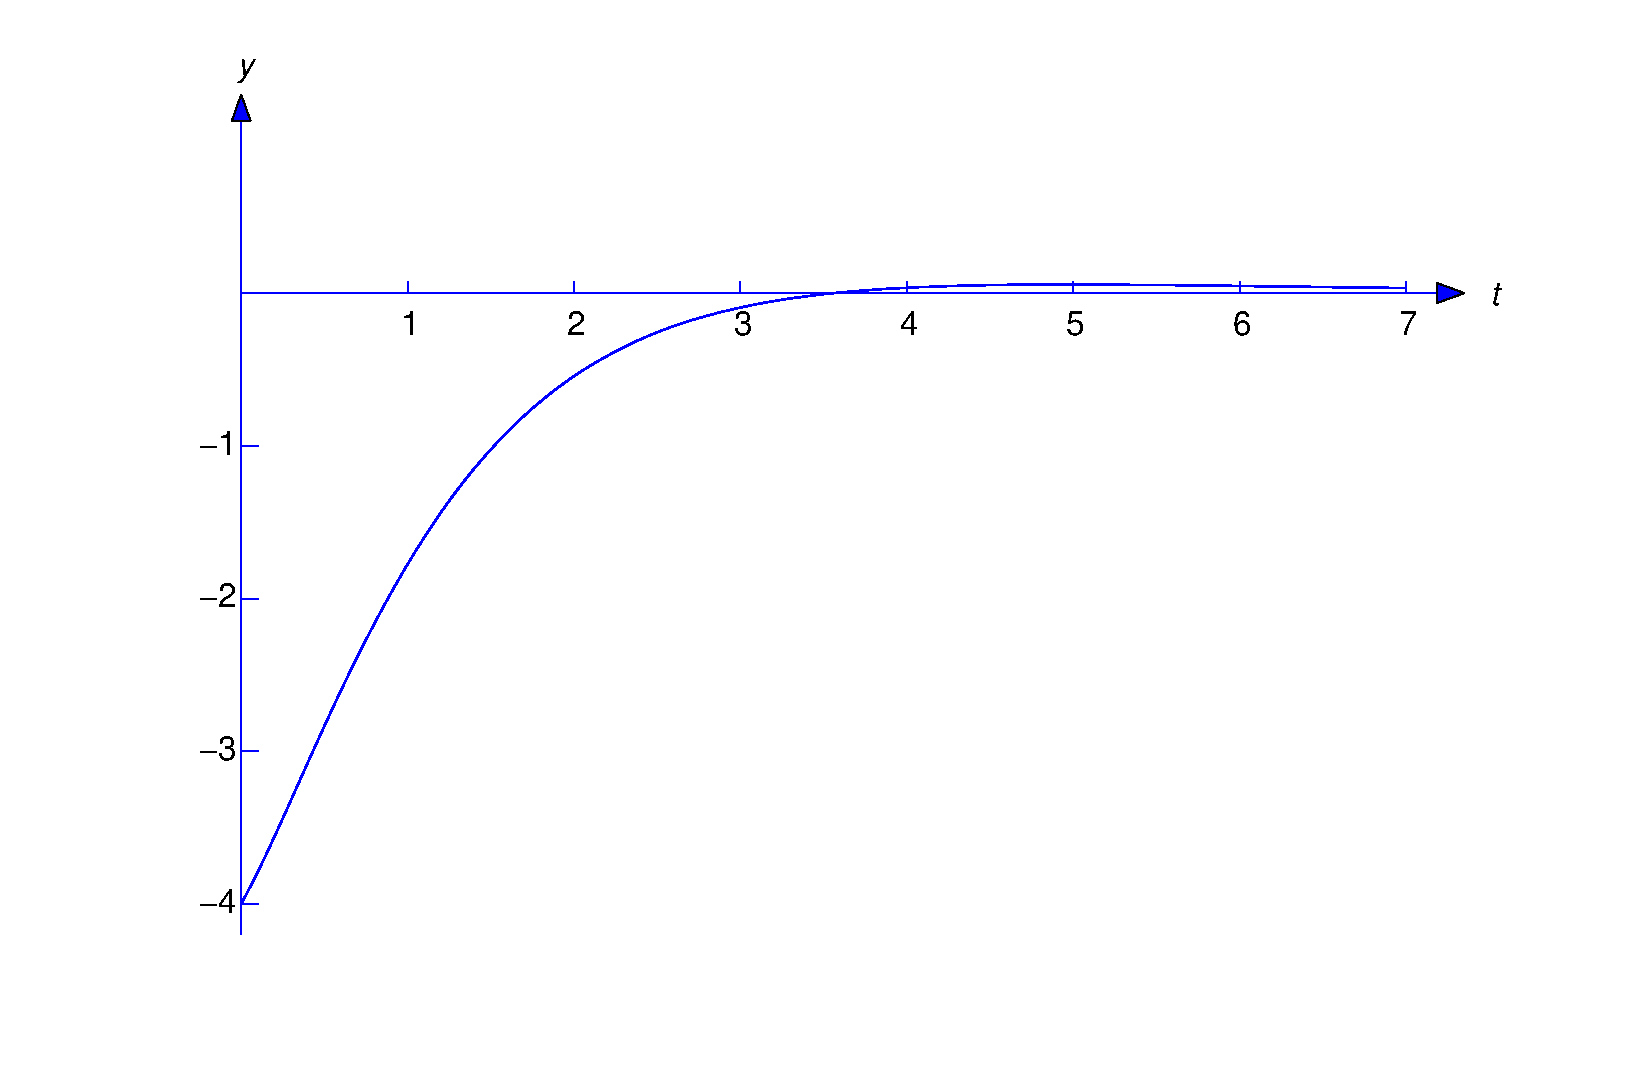
\includegraphics[bb=-78 148 689 643, width=5.67in, height=3.66in, keepaspectratio]{fig080301}}
    \caption{$y=\dst{\frac{4}{3}e^{-t/2}-8e^{-t}+\frac{8}{3}e^{-2t}}$}
    \label{figure:8.3.1}
  \end{minipage}
  \begin{minipage}[b]{0.5\linewidth}
    \centering
    \scalebox{.65}{
    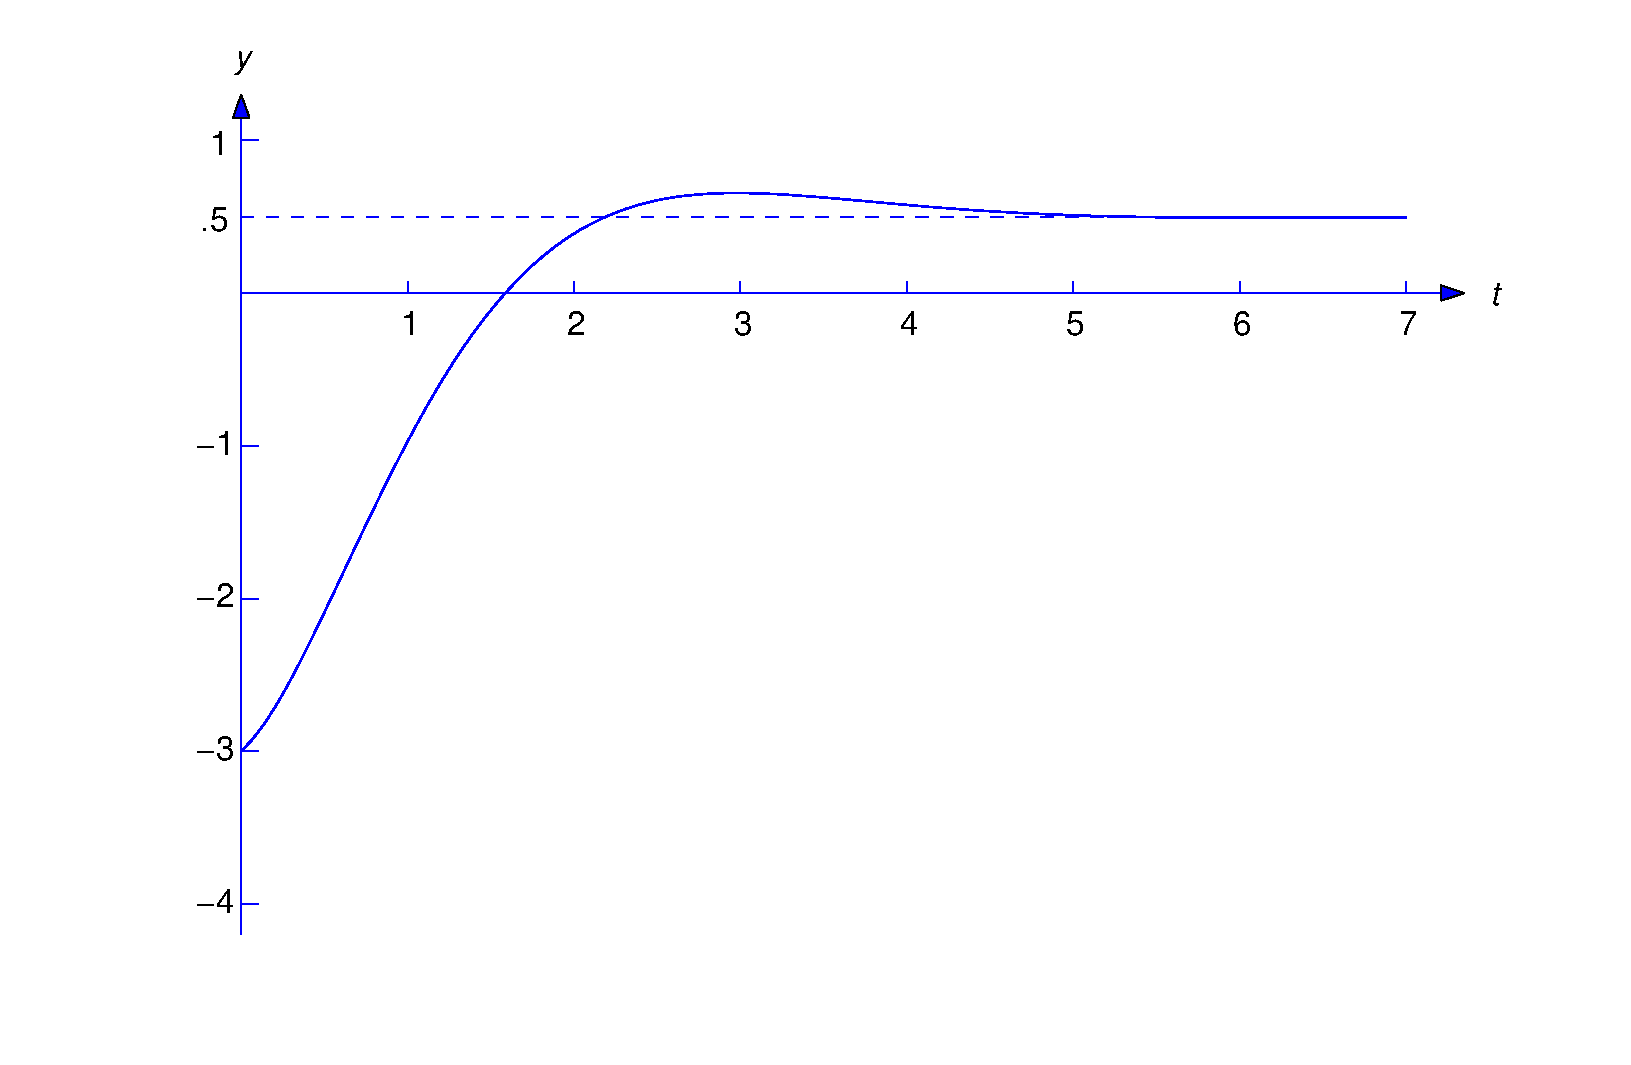
\includegraphics[bb=-78 148 689 643, width=5.67in, height=3.66in, keepaspectratio]{fig080302}}
    \caption{$y=\dst{\frac{1}{2}-\frac{7}{2}e^{-t}\cos t-\frac{5}{2}e^{-t}\sin t}$}
    \label{figure:8.3.2}
  \end{minipage}
\end{figure}

\begin{example}
  \label{example:8.3.4}\rm Solve the initial value problem
  \begin{equation}
    \label{eq:8.3.15}y''+2y'+2y=1,\quad y(0)=-3,\;y'(0)=1.
  \end{equation}
\end{example}

\solution The characteristic polynomial is
\[
  p(s)=s^{2}+2s+2=(s+1)^{2}+1
\]
and
\[
  F(s)={\cal L}(1)=\frac{1}{s},
\]
so \eqref{eq:8.3.13} becomes
\[
  \left[(s+1)^{2}+1\right]Y(s)=\frac{1}{s}+1\cdot(1-3s)+2(-3).
\]
Solving for $Y(s)$ yields
\[
  Y(s)=\frac{1-s(5+3s)}{s\left[(s+1)^{2}+1\right]}.
\]
In Example~\ref{example:8.2.8} we found the inverse transform of this function to be
\[
  y=\frac{1}{2}-\frac{7}{2}e^{-t}\cos t-\frac{5}{2}e^{-t}\sin t
\]
(Figure~\ref{figure:8.3.2}), which is therefore the solution of \eqref{eq:8.3.15}.

\medskip

\color{blue}
\remark{ In our examples we applied Theorems~\ref{thmtype:8.3.1} and \ref{thmtype:8.3.2} without
verifying that the unknown function $y$ satisfies their hypotheses. This is characteristic of the
formal manipulative way in which the Laplace transform is used to solve differential equations. Any
doubts about the validity of the method for solving a given equation can be resolved by verifying
that the resulting function $y$ is the solution of the given problem.}
\color{black}

\exercises In Exercises~\ref{exer:8.3.1}--\ref{exer:8.3.31} use the Laplace transform to solve the initial value problem.

\begin{exerciselist}
  \item\label{exer:8.3.1} $y''+3y'+2y=e^{t},\quad y(0)=1,\quad y'(0)=-6$

  \item\label{exer:8.3.2} $y''-y'-6y=2,\quad y(0)=1,\quad y'(0)=0$

  \item\label{exer:8.3.3} $y''+y'-2y=2e^{3t},\quad y(0)=-1,\quad y'(0)=4$

  \item\label{exer:8.3.4} $y''-4y=2e^{3t},\quad y(0)=1,\quad y'(0)=-1$

  \item\label{exer:8.3.5} $y''+y'-2y=e^{3t},\quad y(0)=1,\quad y'(0)=-1$

  \item\label{exer:8.3.6} $y''+3y'+2y=6e^{t},\quad y(0)=1,\quad y'(0)=-1$

  \item\label{exer:8.3.7} $y''+y=\sin2t,\quad y(0)=0,\quad y'(0)=1$

  \item\label{exer:8.3.8} $y''-3y'+2y=2e^{3t},\quad y(0)=1,\quad y'(0)=-1$

  \item\label{exer:8.3.9} $y''-3y'+2y=e^{4t},\quad y(0)=1,\quad y'(0)=-2$

  \item\label{exer:8.3.10} $y''-3y'+2y=e^{3t},\quad y(0)=-1,\quad y'(0)=-4$

  \item\label{exer:8.3.11} $y''+3y'+2y=2e^{t},\quad y(0)=0,\quad y'(0)=-1$

  \item\label{exer:8.3.12} $y''+y'-2y=-4,\quad y(0)=2,\quad y'(0)=3$

  \item\label{exer:8.3.13} $y''+4y=4,\quad y(0)=0,\quad y'(0)=1$

  \item\label{exer:8.3.14} $y''-y'-6y=2,\quad y(0)=1,\quad y'(0)=0$

  \item\label{exer:8.3.15} $y''+3y'+2y=e^{t},\quad y(0)=0,\quad y'(0)=1$

  \item\label{exer:8.3.16} $y''-y=1,\quad y(0)=1,\quad y'(0)=0$

  \item\label{exer:8.3.17} $y''+4y=3\sin t,\quad y(0)=1,\quad y'(0)=-1$

  \item\label{exer:8.3.18} $y''+y'=2e^{3t},\quad y(0)=-1,\quad y'(0)=4$

  \item\label{exer:8.3.19} $y''+y=1,\quad y(0)=2,\quad y'(0)=0$

  \item\label{exer:8.3.20} $y''+y=t,\quad y(0)=0,\quad y'(0)=2$

  \item\label{exer:8.3.21} $y''+y=t-3\sin2t,\quad y(0)=1,\quad y'(0)=-3$

  \item\label{exer:8.3.22} $y''+5y'+6y=2e^{-t},\quad y(0)=1,\quad y'(0)=3$

  \item\label{exer:8.3.23} $y''+2y'+y=6\sin t-4\cos t,\quad y(0)=-1,\; y'(0)=1$

  \item\label{exer:8.3.24} $y''-2y'-3y=10\cos t,\quad y(0)=2,\quad y'(0)=7$

  \item\label{exer:8.3.25} $y''+y=4\sin t+6\cos t,\quad y(0)=-6,\; y'(0)=2$

  \item\label{exer:8.3.26} $y''+4y=8\sin2t+9\cos t,\quad y(0)=1,\quad y'(0)=0$

  \item\label{exer:8.3.27} $y''-5y'+6y=10e^{t}\cos t,\quad y(0)=2,\quad y'(0)=1$

  \item\label{exer:8.3.28} $y''+2y'+2y=2t,\quad y(0)=2,\quad y'(0)=-7$

  \item\label{exer:8.3.29} $y''-2y'+2y=5\sin t+10\cos t,\quad y(0)=1,\; y'(0)=2$

  \item\label{exer:8.3.30} $y''+4y'+13y=10e^{-t}-36e^{t},\quad y(0)=0,\; y'(0)=-16$

  \item\label{exer:8.3.31} $y''+4y'+5y=e^{-t}(\cos t+3\sin t),\quad y(0)=0,\quad y'(0)=4$

  \item\label{exer:8.3.32} $2y''-3y'-2y=4e^{t},\quad y(0)=1,\;y'(0)=-2$

  \item\label{exer:8.3.33} $6y''-y'-y=3e^{2t},\quad y(0)=0,\;y'(0)=0$

  \item\label{exer:8.3.34} $2y''+2y'+y=2t,\quad y(0)=1,\;y'(0)=-1$

  \item\label{exer:8.3.35} $4y''-4y'+5y=4\sin t-4\cos t,\quad y(0)=0,\;y'(0)=11/17$

  \item\label{exer:8.3.36} $4y''+4y'+y=3\sin t+\cos t,\quad y(0)=2,\;y'(0)=-1$

  \item\label{exer:8.3.37} $9y''+6y'+y=3e^{3t},\quad y(0)=0,\;y'(0)=-3$

  \item\label{exer:8.3.38} Suppose $a$, $b$, and $c$ are constants and $a\ne0$. Let
  \[
    y_{1}={\cal L}^{-1}\left(\frac{as+b}{as^{2}+bs+c}\right)\mbox{\quad and \quad}y_{2}={\cal L}^{-1}\left(\frac{a}{as^{2}+bs+c}\right).
  \]
  Show that
  \[
    y_{1}(0)=1,\quad y_{1}'(0)=0\mbox{\quad and \quad}y_{2}(0)=0,\quad y_{2}'(0)=1.
  \]
  \hint{Use the Laplace transform to solve the initial value problems \begin{eqnarray*}ay''+by'+cy&=&0,\quad y(0)=1,\quad y'(0)=0\\ ay''+by'+cy&=&0,\quad y(0)=0,\quad y'(0)=1.\end{eqnarray*}}
\end{exerciselist}


\section{The Unit Step Function}

\noindent
In the next section we'll consider initial value problems
$$
ay''+by'+cy=f(t),\quad y(0)=k_0,\quad y'(0)=k_1,
$$
where $a$, $b$, and $c$ are constants and $f$ is  piecewise continuous.
 In this section we'll develop procedures for using the
table of Laplace transforms to find  Laplace transforms of
piecewise continuous functions, and to find the piecewise continuous
inverses of Laplace transforms.

\begin{example}\label{example:8.4.1}\rm
 Use the table of Laplace transforms to find the Laplace
transform of
\begin{equation} \label{eq:8.4.1}
f(t)=\left\{\begin{array}{cl}
2t+1,&0\le t<2,\\[1\jot]
 3t,&t\ge2
\end{array}\right.
\end{equation}
(Figure~\ref{figure:8.4.1}).
\end{example}

\solution Since the formula for $f$ changes at $t=2$, we write
\begin{equation}\label{eq:8.4.2}
\begin{array}{ccl}
{\cal L}(f)&=&\dst \int_0^\infty e^{-st}f(t)\,dt\\[2\jot]
&=&\dst\int_0^2 e^{-st}(2t+1)\,dt+\int_2^\infty e^{-st}(3t)\,dt.
\end{array}
\end{equation}
To relate the first term to a Laplace transform,  we   add and subtract
$$
\int_2^\infty e^{-st}(2t+1)\,dt
$$
in \eqref{eq:8.4.2} to obtain
\begin{equation}\label{eq:8.4.3}
\begin{array}{ccl}
{\cal L}(f)&=&\dst\int_0^\infty e^{-st}(2t+1)\,dt+
\int_2^\infty e^{-st}(3t-2t-1)\,dt\\[2\jot]
&=&\dst\int_0^\infty e^{-st}(2t+1)\,dt+
\int_2^\infty e^{-st}(t-1)\,dt\\[2\jot]
&=&\dst{\cal L}(2t+1)+\int_2^\infty e^{-st}(t-1)\,dt.
\end{array}
\end{equation}
To relate  the last integral to a Laplace transform,
  we make the change of variable
 $x=t-2$   and rewrite the integral as
\begin{eqnarray*}
\int_2^\infty e^{-st}(t-1)\,dt&=&\int_0^\infty e^{-s(x+2)}(x+1)\,dx
\\[2\jot]
&=&e^{-2s}\int_0^\infty e^{-sx}(x+1)\,dx.
\end{eqnarray*}
Since the symbol used for the variable of integration has no effect on the
value of a definite integral, we can now replace $x$ by the more standard
$t$ and write
$$
\int_2^\infty e^{-st}(t-1)\,dt
=e^{-2s}\int_0^\infty e^{-st}(t+1)\,dt=e^{-2s}{\cal L}(t+1).
$$
This and \eqref{eq:8.4.3} imply that
$$
{\cal L}(f)={\cal L}(2t+1)+e^{-2s}{\cal L} (t+1).
$$
Now we can use the table of Laplace transforms to find that
$$
{\cal L}(f)={2\over s^2}+{1\over s} +e^{-2s}\left({1\over s^2}+{1\over
s}\right).\bbox
$$

\begin{figure}[H]
\color{blue}
  \begin{minipage}[b]{0.5\linewidth}
    \centering
   \scalebox{.65}{
  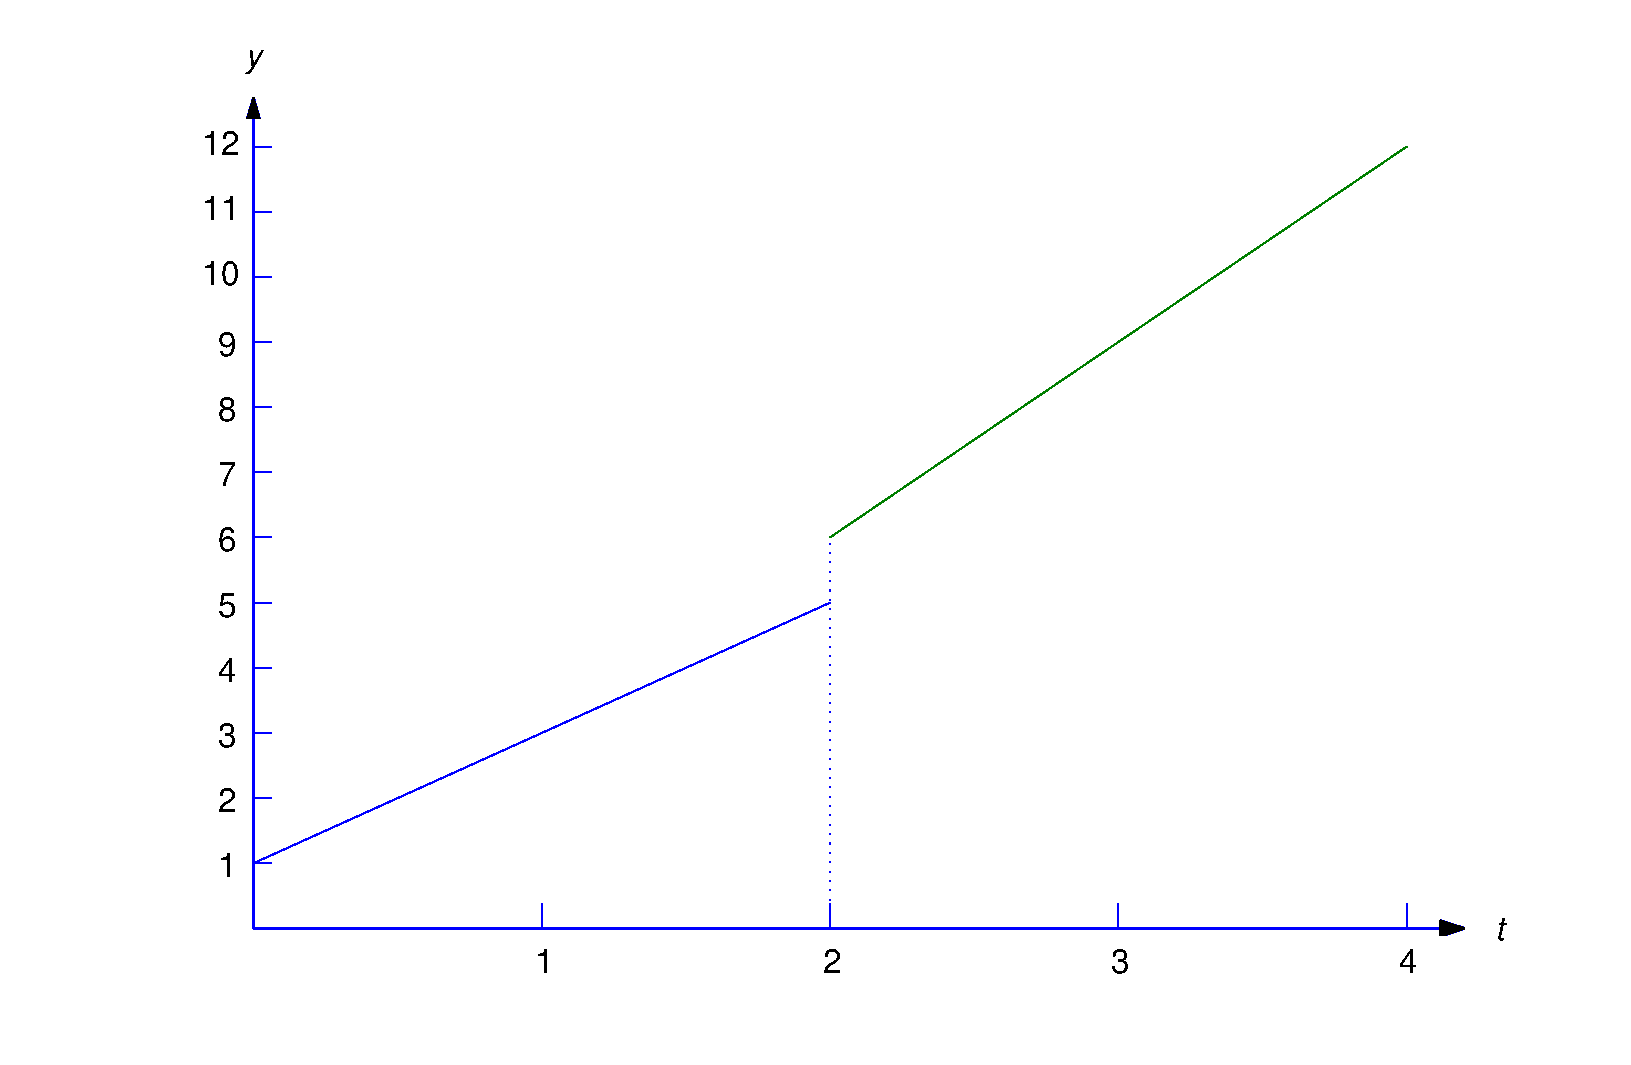
\includegraphics[bb=-78 148 689 643,width=5.67in,height=3.66in,keepaspectratio]{fig080401}}
\caption{The piecewise
 continuous function \eqref{eq:8.4.1}}
  \label{figure:8.4.1}
\end{minipage}
  \begin{minipage}[b]{0.5\linewidth}
    \centering
   \scalebox{.65}{
  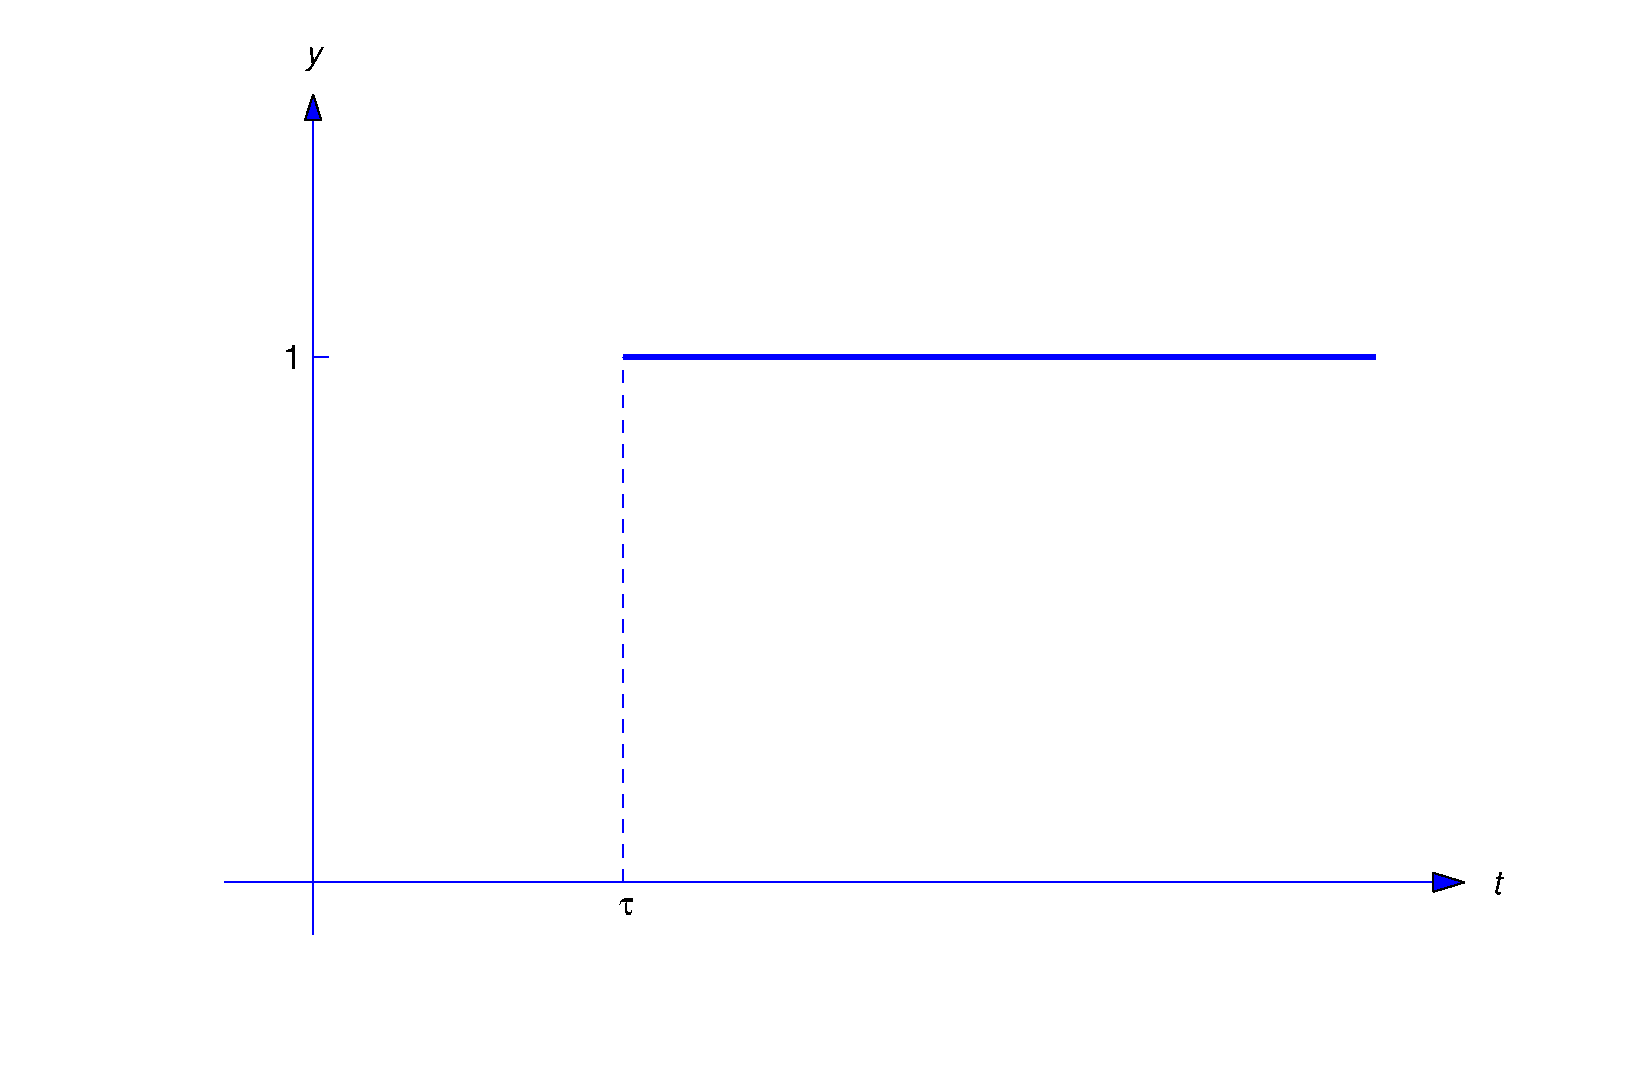
\includegraphics[bb=-78 148 689 643,width=5.67in,height=3.66in,keepaspectratio]{fig080402}}
\caption{ $y=u(t-\tau)$}
  \label{figure:8.4.2}
\end{minipage}
\end{figure}

\boxit{Laplace Transforms of Piecewise Continuous Functions}

\noindent
We'll now develop the method of Example~\ref{example:8.4.1} into a
systematic way to find the Laplace transform of a piecewise continuous
function. It is convenient to introduce the {\color{blue}\it unit step
function\/}, defined as
\begin{equation}\label{eq:8.4.4}
u(t)=\left\{\begin{array}{rl}
0,&t<0\\
1,&t\ge0.
\end{array}\right.
\end{equation}
Thus, $u(t)$ ``steps'' from the constant value $0$ to the constant
value $1$ at $t=0$. If we replace $t$ by
$t-\tau$ in \eqref{eq:8.4.4}, then
$$
u(t-\tau)=\left\{\begin{array}{rl}
0,&t<\tau,\\
1,&t\ge\tau
\end{array}\right.;
$$
that is, the step now occurs at $t=\tau$ (Figure~\ref{figure:8.4.2}).

The step function enables us to represent piecewise continuous
functions conveniently. For example, consider the function
\begin{equation}\label{eq:8.4.5}
f(t)=\left\{\begin{array}{rl}
f_0(t),&0\le t<t_1,\\[1\jot]
f_1(t),&t\ge t_1,
\end{array}\right.
\end{equation}
where we assume that $f_0$ and $f_1$ are defined on $[0,\infty)$, even
though they equal $f$ only on the indicated intervals. This assumption
enables us to rewrite \eqref{eq:8.4.5} as
\begin{equation}\label{eq:8.4.6}
f(t)=f_0(t)+u(t-t_1)\left(f_1(t)-f_0(t)\right).
\end{equation}
To verify this, note that if $t<t_1$ then $u(t-t_1)=0$ and
\eqref{eq:8.4.6}  becomes
$$
f(t)=f_0(t)+(0)\left(f_1(t)-f_0(t)\right)=f_0(t).
$$
If $t\ge t_1$ then $u(t-t_1)=1$ and  \eqref{eq:8.4.6} becomes
$$
f(t)=f_0(t)+(1)\left(f_1(t)-f_0(t)\right)=f_1(t).
$$

We need the next theorem to
 show how \eqref{eq:8.4.6} can be used to find ${\cal L}(f)$.

\begin{theorem}\color{blue}\label{thmtype:8.4.1}
Let $g$ be defined on $[0,\infty).$ Suppose   $\tau\ge0$ and ${\cal
L}\left(g(t+\tau)\right)$ exists for $s>s_0.$ Then ${\cal
L}\left(u(t-\tau)g(t)\right)$ exists for $s>s_0$, and
$$
{\cal L}(u(t-\tau)g(t))=e^{-s\tau}{\cal L}\left(g(t+\tau)\right).
$$
\end{theorem}

\proof By definition,
$$
{\cal L}\left(u(t-\tau)g(t)\right)=\int_0^\infty e^{-st} u(t-\tau)g(t)\,
dt.
$$
From this and the definition of $u(t-\tau)$,
$$
{\cal L}\left(u(t-\tau)g(t)\right)=\int_0^\tau
e^{-st}(0)\,dt+\int_{\tau}^\infty e^{-st}g(t)\,dt.
$$
The first integral on the right equals zero.  Introducing the new variable
of integration $x=t-\tau$ in the second integral yields
$$
{\cal L}\left(u(t-\tau)g(t)\right)=\int_0^\infty e^{-s(x+\tau)}g(x+\tau)\,dx
=e^{-s\tau}\int_0^\infty e^{-sx} g(x+\tau)\,dx.
$$
Changing the name of the variable of integration in the last integral
from $x$ to $t$ yields
$$
{\cal L}\left(u(t-\tau)g(t)\right)
=e^{-s\tau}\int_0^\infty e^{-st} g(t+\tau)\,dt=e^{-s\tau}{\cal
L}(g(t+\tau)).\bbox
$$

\begin{example}\label{example:8.4.2}\rm
 Find
$$
{\cal L}\left(u(t-1)(t^2+1)\right).
$$
\end{example}

\solution  Here $\tau=1$ and $g(t)=t^2+1$, so
$$
g(t+1)=(t+1)^2+1=t^2+2t+2.
$$
Since
$$
{\cal L}\left(g(t+1)\right)={2\over s^3}+{2\over s^2}+{2\over s},
$$
Theorem~\ref{thmtype:8.4.1} implies that
$${\cal L}\left(u(t-1)(t^2+1)\right)
=e^{-s}\left({2\over s^3}+{2\over s^2}+{2\over s}\right).
$$

\begin{example}\label{example:8.4.3}\rm
Use Theorem~\ref{thmtype:8.4.1} to find the Laplace transform of the
function
$$
f(t)=\left\{\begin{array}{cl} 2t+1,&0\le t<2,\\[1\jot] 3t,&t\ge2,
\end{array}\right.
$$
from Example~\ref{example:8.4.1}.
\end{example}

\solution
We first write $f$ in the form \eqref{eq:8.4.6} as
$$
f(t)=2t+1+u(t-2)(t-1).
$$
Therefore
\begin{eqnarray*}
{\cal L}(f)&=&{\cal L}(2t+1) +{\cal L}\left(u(t-2)(t-1)\right)\\
&=&{\cal L}(2t+1) +e^{-2s}{\cal L}(t+1)\quad\mbox{ (from
Theorem~\ref{thmtype:8.4.1}})\\
&=&{2\over s^2}+{1\over s}+e^{-2s}\left({1\over s^2}+{1\over s}\right),
\end{eqnarray*}
which is the result obtained in Example~\ref{example:8.4.1}.\bbox

Formula \eqref{eq:8.4.6} can be extended to more general piecewise continuous
functions. For example, we can write
$$
f(t)=\left\{\begin{array}{rl}
f_0(t),&0\le t<t_1,\\[1\jot]
f_1(t),&t_1\le t<t_2,\\[1\jot]
f_2(t),&t\ge t_2,
\end{array}\right.
$$
as
$$
f(t)=f_0(t)+u(t-t_1)\left(f_1(t)-f_0(t)\right)+
u(t-t_2)\left(f_2(t)-f_1(t)\right)
$$
if $f_0$, $f_1$, and $f_2$ are all defined on $[0,\infty)$.

\begin{example}\label{example:8.4.4}\rm
 Find the Laplace transform of
\begin{equation} \label{eq:8.4.7}
f(t)=\left\{\begin{array}{cl}
 1,&0\le t<2,\\[1\jot]
-2t+1,&2\le t<3,\\[1\jot]
 3t,&3\le t<5,\\[1\jot]
 t-1,&t\ge5
\end{array}\right.
\end{equation}
(Figure~\ref{figure:8.4.3}).
\end{example}

\begin{figure}[tbp]
  \centering\color{blue}
  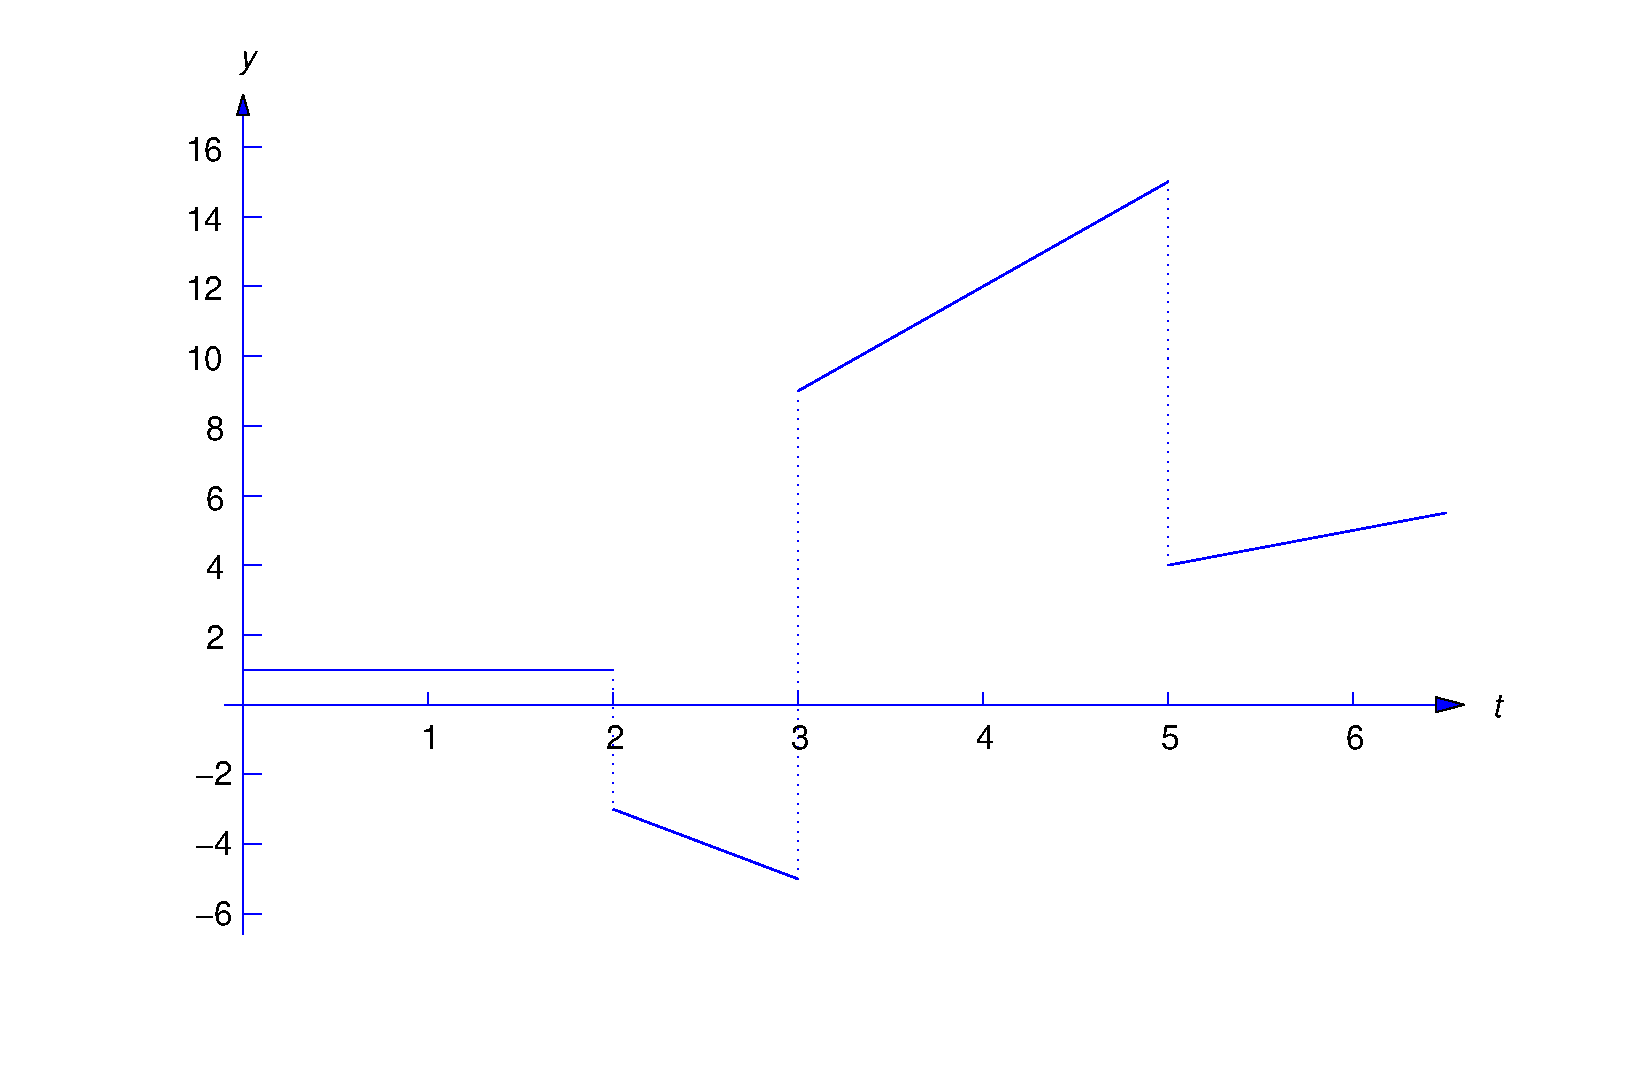
\includegraphics[bb=-78 148 689 643,width=5.67in,height=3.66in,keepaspectratio]{fig080403}
  \caption{The piecewise continuous function \eqref{eq:8.4.7}}
  \label{figure:8.4.3}
\end{figure}

\solution   In terms of step functions,
\begin{eqnarray*}
f(t)&=&1+u(t-2)(-2t+1-1)+u(t-3)(3t+2t-1)\\
&&+u(t-5)(t-1-3t),
\end{eqnarray*}
or
$$
f(t)=1-2u(t-2)t+u(t-3)(5t-1)-u(t-5)(2t+1).
$$
Now Theorem~\ref{thmtype:8.4.1} implies that
\begin{eqnarray*}
{\cal L}(f)&=&{\cal L}(1)-2e^{-2s}{\cal L}(t+2)+e^{-3s}{\cal
L}\left(5(t+3)-1\right)-e^{-5s}{\cal L}\left(2(t+5)+1\right)\\[1\jot]
&=&{\cal L}(1)-2e^{-2s}{\cal L}(t+2)+e^{-3s}{\cal
L}(5t+14)-e^{-5s}{\cal L}(2t+11)\\[1\jot]
&=&{1\over s}-2e^{-2s}\left({1\over s^2}+{2\over s}\right)+
e^{-3s}\left({5\over s^2}+{14\over s}\right)-e^{-5s}\left({2\over
s^2}+{11\over s}\right).\bbox
\end{eqnarray*}

 The trigonometric identities
\begin{eqnarray}
\sin (A+B)&=&\sin A\cos B+\cos A\sin B\label{eq:8.4.8}\\
\cos (A+B)&=&\cos A\cos B-\sin A\sin B\label{eq:8.4.9}
\end{eqnarray}
are useful in problems that involve shifting the arguments of
trigonometric functions. We'll use these identities in the next
example.

\begin{example}\label{example:8.4.5}\rm
 Find the Laplace transform of
\begin{equation} \label{eq:8.4.10}
f(t)=\left\{\begin{array}{cl}
\sin t,&0\le t<\dst{\pi\over 2},\\[2\jot]
\cos t-3\sin t,&\dst{\pi\over 2}\le t<\pi,\\[2\jot]
 3\cos t,&t\ge\pi
\end{array}\right.
\end{equation}
(Figure~\ref{figure:8.4.4}).
\end{example}

                 %
\begin{figure}[tbp]
  \centering\color{blue}
  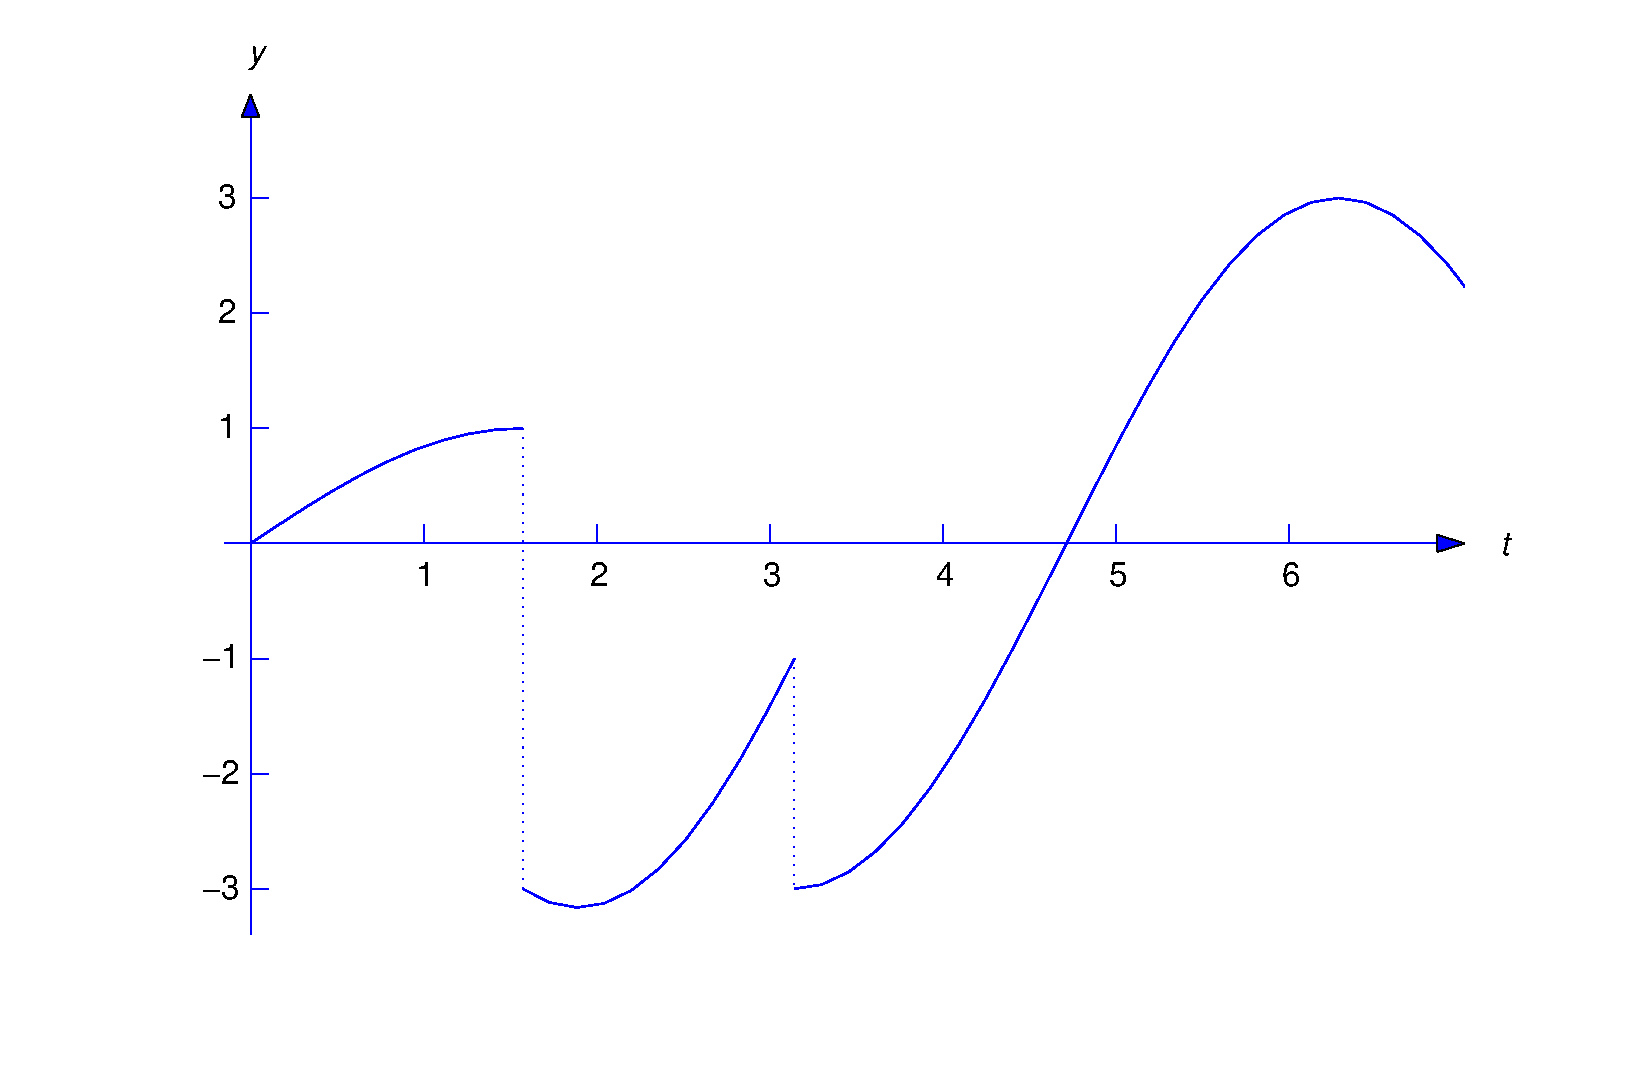
\includegraphics[bb=-78 148 689 643,width=5.67in,height=3.66in,keepaspectratio]{fig080404}
  \caption{The piecewise continuous function \eqref{eq:8.4.10}}
  \label{figure:8.4.4}
\end{figure}

 \solution In terms of step functions,
$$
f(t)=\sin t+u(t-\pi/2) (\cos t-4\sin t)+u(t-\pi) (2
\cos t+3\sin t).
$$
Now Theorem~\ref{thmtype:8.4.1} implies that
\begin{equation}\label{eq:8.4.11}
\begin{array}{ccl}
{\cal L}(f)&=&{\cal L}(\sin t)+e^{-{\pi\over 2}s}{\cal L}
\left(\cos\left(t+{\pi\over2}\right)-4\sin\left(t+{\pi\over2}\right)\right)\\
[1\jot]&&\qquad+e^{-\pi s}{\cal L}\left(2\cos(t+\pi)+3\sin(t+\pi)\right).
\end{array}
\end{equation}
Since
$$
\cos\left(t+{\pi\over 2}\right)-4\sin\left(t+{\pi\over
2}\right)=-\sin t-4\cos t
$$
and
$$
 2\cos (t+\pi)+3\sin (t+\pi)=-2\cos t-3\sin t,
$$
we see from \eqref{eq:8.4.11} that
\begin{eqnarray*}
{\cal L}(f)&=&{\cal L}(\sin t)-e^{-\pi s/2}{\cal L}(\sin t+4\cos t)
-e^{-\pi s}{\cal L}(2\cos t+3\sin t)\\[1\jot]
&=&{1\over s^2+1}-e^{-{\pi\over 2}s}\left({1+4s\over
s^2+1}\right)
-e^{-\pi s}\left({3+2s\over s^2+1}\right).\bbox
\end{eqnarray*}

\boxit{The Second Shifting Theorem}

\noindent
Replacing $g(t)$ by $g(t-\tau)$ in Theorem~\ref{thmtype:8.4.1}
yields the next theorem.

\begin{theorem}\color{blue}$[$Second Shifting
Theorem$]$\label{thmtype:8.4.2} If
 $\tau\ge0$ and ${\cal L}(g)$ exists for $s>s_0$
then  ${\cal L}\left(u(t-\tau)g(t-\tau)\right)$ exists for $s>s_0$ and
$$
{\cal L}(u(t-\tau)g(t-\tau))=e^{-s\tau}{\cal L}(g(t)),
$$
or, equivalently,
\begin{equation}\label{eq:8.4.12}
\mbox{if } g(t)\leftrightarrow G(s),\mbox{ then
}u(t-\tau)g(t-\tau)\leftrightarrow e^{-s\tau}G(s).
\end{equation}
\end{theorem}

\color{blue}
\remark{ Recall that the First Shifting Theorem
(Theorem~\ref{thmtype:8.1.3} states that multiplying a function  by
$e^{at}$ corresponds to shifting the argument of its transform by $a$
units. Theorem~\ref{thmtype:8.4.2} states that multiplying a Laplace
transform by the exponential $e^{-\tau s}$ corresponds to shifting the
argument of the inverse transform by $\tau$ units.}
\color{black}

\begin{example}\label{example:8.4.6}\rm
 Use \eqref{eq:8.4.12} to find
$$
{\cal L}^{-1}\left(e^{-2s}\over s^2\right).
$$
\end{example}

\solution  To apply \eqref{eq:8.4.12} we let
$\tau=2$ and $G(s)=1/s^2$. Then $g(t)=t$ and \eqref{eq:8.4.12} implies that
$$
{\cal L}^{-1}\left(e^{-2s}\over s^2\right)=u(t-2)(t-2).\bbox
$$

\begin{example}\label{example:8.4.7}\rm
 Find the inverse Laplace transform $h$ of
$$
H(s)={1\over s^2}-e^{-s}\left({1\over s^2}+{2\over s}\right)+
e^{-4s}\left({4\over s^3}+{1\over s}\right),
$$
and find distinct formulas for $h$ on appropriate intervals.
\end{example}

\solution  Let
$$
G_0(s)={1\over s^2},\quad G_1(s)={1\over s^2}+{2\over s},\quad
G_2(s)={4\over s^3}+{1\over s}.
$$
Then
$$
g_0(t)=t,\; g_1(t)=t+2,\; g_2(t)=2t^2+1.
$$
Hence, \eqref{eq:8.4.12} and the linearity of ${\cal L}^{-1}$ imply that
\begin{eqnarray*}
h(t)&=&{\cal L}^{-1}\left(G_0(s)\right)-{\cal
L}^{-1}\left(e^{-s}G_1(s)\right)+{\cal
L}^{-1}\left(e^{-4s}G_2(s)\right)\\[1\jot]
&=&t-u(t-1)\left[(t-1)+2\right]+u(t-4)\left[2(t-4)^2+1\right]\\[1\jot]
&=&t-u(t-1)(t+1)+u(t-4)(2t^2-16t+33),
\end{eqnarray*}
which can also be written as
$$
h(t)=\left\{\begin{array}{cl}
 t,&0\le t<1,\\[1\jot]
-1,&1\le t<4,\\[1\jot]
2t^2-16t+32,&t\ge4.
\end{array}\right.\bbox
$$

\begin{example}\label{example:8.4.8}\rm
 Find the inverse transform of
$$
H(s)={2s\over s^2+4}-e^{-{\pi\over 2}s} {3s+1\over s^2+9}+e^{-\pi
s}{s+1\over s^2+6s+10}.
$$
\end{example}

\solution  Let
$$
G_0(s)={2s\over s^2+4},\quad G_1(s)=-{(3s+1)\over s^2+9},
$$
and
$$
G_2(s)={s+1\over s^2+6s+10}={(s+3)-2\over (s+3)^2+1}.
$$
Then
$$
g_0(t)=2\cos 2t,\quad g_1(t)=-3\cos 3t-{1\over 3}\sin 3t,
$$
and
$$
g_2(t)=e^{-3t}(\cos t-2\sin t).
$$
Therefore \eqref{eq:8.4.12} and the linearity of ${\cal L}^{-1}$
imply that
\begin{eqnarray*}
h(t)&=&2\cos 2t-u(t-\pi/2)\left[3\cos
3(t-\pi/2)+{1\over 3}\sin 3\left(t-{\pi\over
2}\right)\right]\\[2\jot]
&&+u(t-\pi)e^{-3(t-\pi)}\left[\cos (t-\pi)-2\sin (t-\pi)\right].
\end{eqnarray*}
Using the trigonometric identities  \eqref{eq:8.4.8} and
\eqref{eq:8.4.9}, we can rewrite this as
\begin{equation} \label{eq:8.4.13}
\begin{array}{rcl}
h(t)&=&2\cos 2t+u(t-\pi/2)\left(3\sin 3t-
{1\over 3}\cos 3t\right)\\[2\jot]
&&-u(t-\pi)e^{-3(t-\pi)} (\cos t-2\sin t)
\end{array}
\end{equation}
(Figure~\ref{figure:8.4.5}).

\begin{figure}[H]
  \centering\color{blue}
  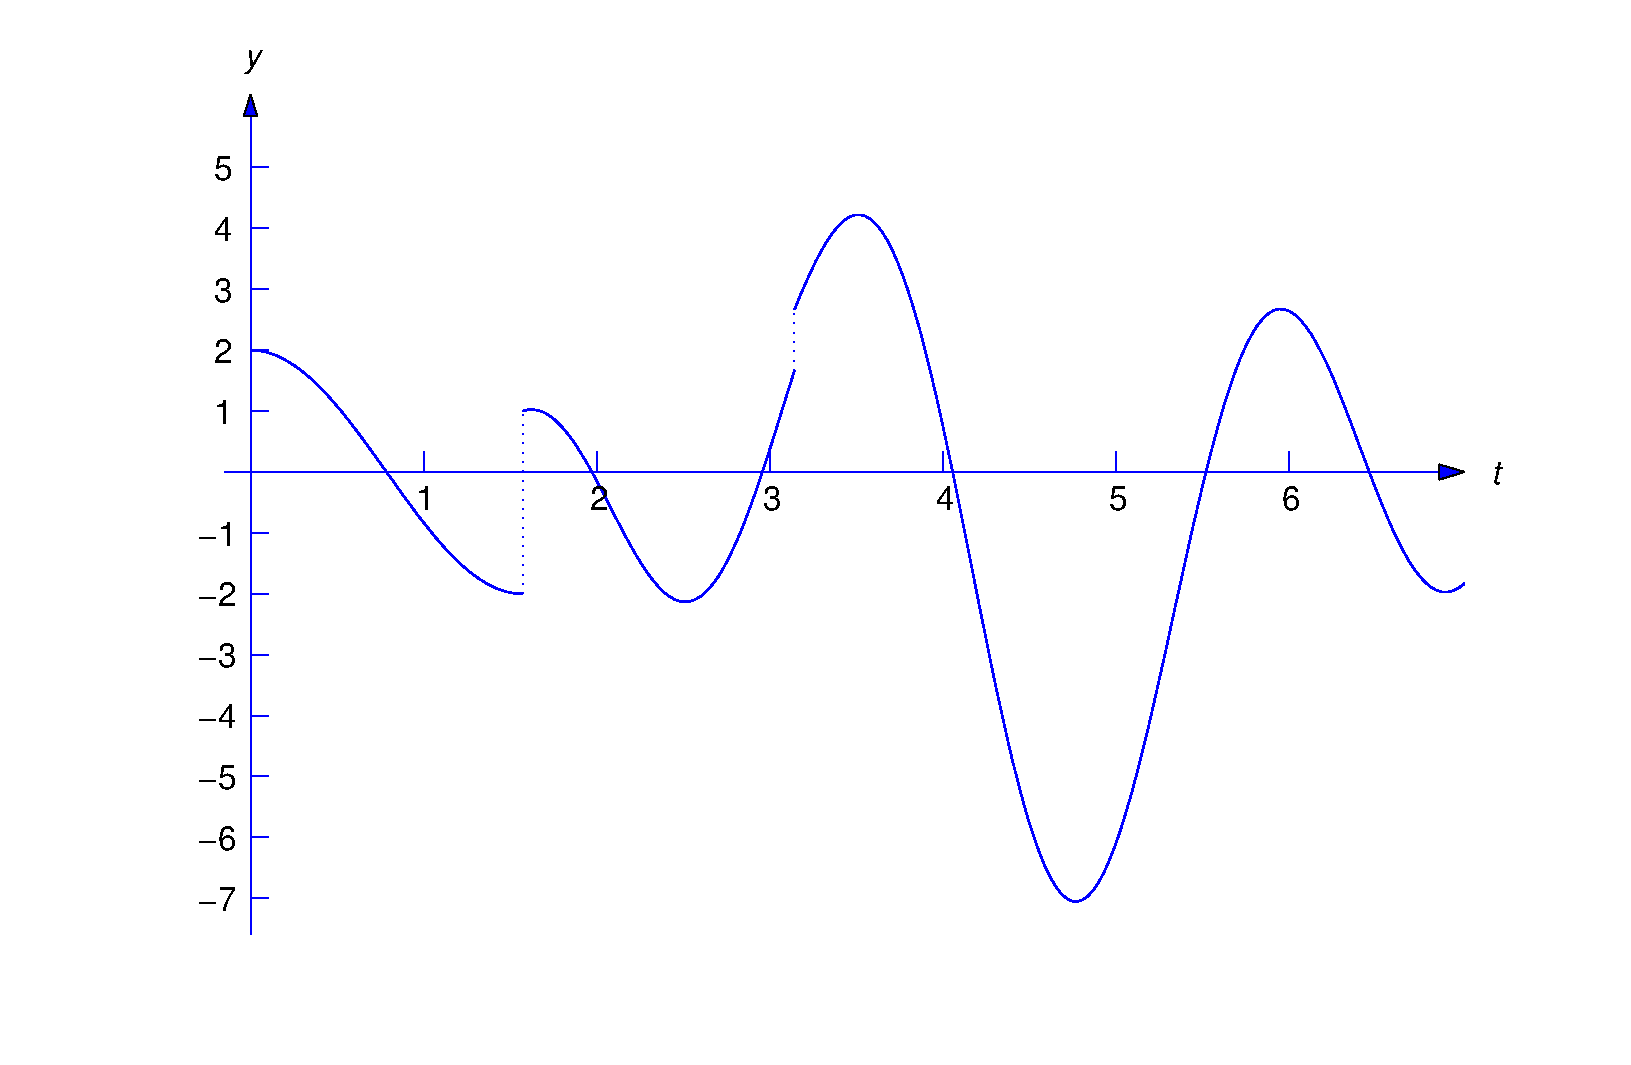
\includegraphics[bb=-78 148 689 643,width=5.67in,height=3.66in,keepaspectratio]{fig080405}
  \caption{ The piecewise continuous function
\eqref{eq:8.4.13}}
  \label{figure:8.4.5}
\end{figure}

 \exercises
In Exercises~\ref{exer:8.4.1}--\ref{exer:8.4.6} find the Laplace transform by
the method of Example~\ref{example:8.4.1}. Then express the given function
$f$ in terms of unit step functions as in Eqn.~\eqref{eq:8.4.6}, and use
Theorem~\ref{thmtype:8.4.1} to find ${\cal L}(f)$.
Where indicated by \CGex, graph $f$.
\begin{exerciselist}

\begin{tabular}[t]{@{}p{168pt}@{}p{168pt}}
\item\label{exer:8.4.1} $\dst{f(t)=\left\{\begin{array}{cl} 1,&0
\le t<4,\\[2\jot] t,&t\ge4.\end{array}\right.}$&
\item\label{exer:8.4.2} $\dst{f(t)=\left\{\begin{array}{cl} t,&0
\le t<1,\\[2\jot] 1,&t\ge1.\end{array}\right.}$
\end{tabular}

\begin{tabular}[t]{@{}p{168pt}@{}p{168pt}}
\item\label{exer:8.4.3} \CGex $\dst{f(t)=\left\{\begin{array}{cl} 2t-1,&
0\le t<2,\\[2\jot]  t,&t\ge2.\end{array}\right.}$&
\item\label{exer:8.4.4} \CGex $\dst{f(t)=\left\{\begin{array}{cl}1,
&0\le t<1,\\[2\jot] t+2,&t\ge1.\end{array}\right.}$
\end{tabular}

\begin{tabular}[t]{@{}p{168pt}@{}p{168pt}}
\item\label{exer:8.4.5}$\dst{f(t)=\left\{\begin{array}{cl} t-1,& 0\le
t<2,\\[2\jot] 4,&t\ge2.\end{array}\right.}$&
\item\label{exer:8.4.6} $\dst{f(t)=\left\{\begin{array}{cl} t^2,& 0\le
t<1,\\[2\jot] 0,&t\ge1.\end{array}\right.}$
\end{tabular}

\exercisetext{In Exercises~\ref{exer:8.4.7}--\ref{exer:8.4.18} express the
given function $f$ in terms of unit step functions
 and use Theorem~\ref{thmtype:8.4.1} to find ${\cal
L}(f)$.
Where indicated by \CGex, graph $f$.}

\begin{tabular}[t]{@{}p{168pt}@{}p{168pt}}
\item\label{exer:8.4.7}$\dst{f(t)=\left\{\begin{array}{cl} 0, &0\le
t<2,\\[2\jot] t^2+3t,&t\ge2.\end{array}\right.}$&
\item\label{exer:8.4.8} $\dst{f(t)=\left\{\begin{array}{cl} t^2+2, &0\le
t<1,\\[2\jot] t,&t\ge1.\end{array}\right.}$
\end{tabular}

\begin{tabular}[t]{@{}p{168pt}@{}p{168pt}}
\item\label{exer:8.4.9} $\dst{f(t)=\left\{\begin{array}{cl} te^t,& 0\le t
<1,\\[2\jot] e^t,&t\ge1.\end{array}\right.}$&
\item\label{exer:8.4.10} $\dst{f(t)=\left\{\begin{array}{cl}
e^{\phantom{2}-t}, &0\le t<1,\\[2\jot]
e^{-2t},&t\ge1.\end{array}\right.}$
\end{tabular}

\begin{tabular}[t]{@{}p{168pt}@{}p{168pt}}
\item\label{exer:8.4.11} $\dst{f(t)=\left\{\begin{array}{cl} -t,&0 \le
t<2,\\[2\jot] t-4,&2\le t<3,\\[2\jot] 1,&t\ge3.
\end{array}\right.}$&
\item\label{exer:8.4.12} $\dst{f(t)=\left\{\begin{array}{cl} 0,&0 \le
t<1,\\[2\jot] t,&1\le t<2,\\[2\jot] 0,&t\ge2.\end{array}\right.}$
\end{tabular}

\begin{tabular}[t]{@{}p{168pt}@{}p{168pt}}
\item\label{exer:8.4.13} $\dst{f(t)=\left\{\begin{array}{cl} t,&0 \le
t<1,\\[2\jot] t^2,&1\le t<2,\\[2\jot] 0,&t\ge2. \end{array}\right.}$&
\item\label{exer:8.4.14} $\dst{f(t)=\left\{\begin{array}{cl} t,&0\le
t<1,\\[2\jot] 2-t,&1\le t<2,\\[2\jot] 6,&t > 2. \end{array}\right.}$
\end{tabular}

\item\label{exer:8.4.15} \CGex $\dst{f(t)=\left\{\begin{array}{cl}
\phantom{2}
\sin t,&0\le t<\dst{\pi\over 2},\\[2\jot] 2\sin t,&
\dst{\pi\over 2}\le t<\pi,\\[2\jot]\phantom{2}\cos t,
&t\ge\pi.\end{array}\right.}$

\item\label{exer:8.4.16} \CGex
$f(t)=\dst{\left\{\begin{array}{cl}\phantom{-} 2,&0\le
t<1,\\[2\jot]-2t+2,&1\le t<3,\\[2\jot]\phantom{-}3t,&t\ge
3.\end{array}\right.}$

\item\label{exer:8.4.17}  \CGex
$f(t)=\dst{\left\{\begin{array}{cl}3,&0\le t<2,\\[2\jot]3t+2,&2\le
t<4,\\[2\jot]4t,&t\ge
4.\end{array}\right.}$

\item\label{exer:8.4.18}  \CGex
$\dst{f(t)=\left\{\begin{array}{ll}(t+1)^2,&0\le t<1,
\\[2\jot](t+2)^2,&t\ge1.\end{array}\right.}$

\exercisetext{In Exercises~\ref{exer:8.4.19}--\ref{exer:8.4.28} use
Theorem~\ref{thmtype:8.4.2} to express the inverse transforms in terms of
step functions, and then find distinct formulas the for inverse
transforms on the appropriate intervals, as in
Example~\ref{example:8.4.7}.
Where indicated by \CGex, graph the inverse transform.}

\begin{tabular}[t]{@{}p{168pt}@{}p{112pt}@{}p{68pt}}
\item\label{exer:8.4.19} $\dst{H(s)={e^{-2s}\over s-2}}$&
\item\label{exer:8.4.20} $\dst{H(s)={e^{-s}\over s(s+1)}}$
\end{tabular}

\item\label{exer:8.4.21} \CGex $\dst{H(s)={e^{-s}\over s^3}+
{e^{-2s}\over s^2}}$

\item\label{exer:8.4.22} \CGex $\dst{H(s)=\left({2\over s}+{1\over s^2}\right)
+e^{-s}\left({3\over s}-{1\over s^2}\right)+e^{-3s}\left({1\over
s}+{1\over s^2}\right)}$

\item\label{exer:8.4.23} $\dst{H(s)=\left({5\over s}-{1\over s^2}\right)
+e^{-3s}\left({6\over s}+{7\over s^2}\right)+{3e^{-6s}\over s^3}}$

\item\label{exer:8.4.24} $\dst{H(s)={e^{-\pi s} (1-2s)\over s^2+4s+5}}$

\item\label{exer:8.4.25} \CGex $\dst{H(s)=\left({1\over s}-{s\over
s^2+1}\right)+e^{-{\pi\over 2}s}\left({3s-1\over s^2+1}\right)}$

\item\label{exer:8.4.26} $\dst{H(s)=
e^{-2s}\left[{3(s-3)\over(s+1)(s-2)}-{s+1\over(s-1)(s-2)}\right]}$

\item\label{exer:8.4.27} $\dst{H(s)={1\over s}+{1\over
s^2}+e^{-s}\left({3\over s}+{2\over s^2}\right) +e^{-3s}\left({4\over
s}+{3\over s^2}\right)}$

\item\label{exer:8.4.28} $\dst{H(s)={1\over s}-{2\over
s^3}+e^{-2s}\left({3\over s}-{1\over s^3}\right) +{e^{-4s}\over s^2}}$

\item\label{exer:8.4.29} Find ${\cal L}\left(u(t-\tau)\right)$.

\item\label{exer:8.4.30}
Let $\{t_m\}_{m=0}^\infty$ be a sequence of points such that $t_0=0$,
$t_{m+1}>t_m$, and $\lim_{m\to\infty}t_m=\infty$. For each nonnegative
integer $m$, let $f_m$ be continuous on $[t_m,\infty)$, and let $f$ be
defined on $[0,\infty)$ by
$$
f(t)=f_m(t),\,t_m\le t<t_{m+1}\quad (m=0,1,\dots).
$$
Show that $f$ is piecewise continuous on $[0,\infty)$  and
that it has the step function representation
$$
f(t)=f_0(t)+\sum_{m=1}^\infty u(t-t_m)\left(f_m(t)-f_{m-1}(t)\right),\,
0\le t<\infty.
$$
How do we know that the series on the right converges for all $t$
in $[0,\infty)$?

\item\label{exer:8.4.31}
In addition to the assumptions of Exercise~\ref{exer:8.4.30},
assume that
$$
|f_m(t)|\le Me^{s_0t},\,t\ge t_m,\,m=0,1,\dots,
\eqno{\rm (A)}
$$
and that the series
$$
\sum_{m=0}^\infty e^{-\rho t_m}
\eqno{\rm (B)}
$$
converges for some $\rho>0$. Using the  steps listed below, show
that
${\cal L}(f)$ is defined for $s>s_0$  and
$$
{\cal L}(f)={\cal L}(f_0)+\sum_{m=1}^\infty e^{-st_m}{\cal L}(g_m)
\eqno{\rm (C)}
$$
for $s>s_0+\rho$,
where
$$
g_m(t)=f_m(t+t_m)-f_{m-1}(t+t_m).
$$

\begin{alist} % (a)
\item
Use (A) and Theorem~8.1.6 to show that
$$
{\cal
L}(f)=\sum_{m=0}^\infty\int_{t_m}^{t_{m+1}}e^{-st}f_m(t)\,dt
\eqno{\rm (D)}
$$
is defined for $s>s_0$.
\item % (b)
Show that  (D) can be rewritten as
$$
{\cal L}(f)=\sum_{m=0}^\infty\left(\int_{t_m}^\infty e^{-st}f_m(t)\,dt
-\int_{t_{m+1}}^\infty e^{-st}f_m(t)\,dt\right).
\eqno{\rm (E)}
$$
\item % (c)
Use  (A), the assumed convergence of  (B), and the
comparison test  to show that the series
$$
\sum_{m=0}^\infty\int_{t_m}^\infty e^{-st}f_m(t)\,dt\mbox{\quad and \quad}
\sum_{m=0}^\infty\int_{t_{m+1}}^\infty e^{-st}f_m(t)\,dt
$$
both converge (absolutely) if $s>s_0+\rho$.
\item % (d)
Show that  (E) can be rewritten as
 $$
{\cal L}(f)={\cal L}(f_0)+\sum_{m=1}^\infty\int_{t_m}^\infty e^{-st}
\left(f_m(t)-f_{m-1}(t)\right)\,dt
$$
if $s>s_0+\rho$.
\item % (e)
Complete the proof of  (C).
\end{alist}

\item\label{exer:8.4.32} Suppose $\{t_m\}_{m=0}^\infty$ and
$\{f_m\}_{m=0}^\infty$ satisfy the assumptions of
Exercises~\ref{exer:8.4.30} and \ref{exer:8.4.31}, and
there's a positive constant $K$ such that $t_m\ge Km$ for $m$
sufficiently large. Show that the series  (B) of
Exercise~\ref{exer:8.4.31} converges for any $\rho>0$, and conclude from
this that  (C) of Exercise~\ref{exer:8.4.31} holds for $s>s_0$.

\exercisetext{In Exercises~\ref{exer:8.4.33}--\ref{exer:8.4.36} find the step
function representation of $f$ and use the result of
Exercise~\ref{exer:8.4.32} to find ${\cal L}(f)$. \hint{You will need
formulas related to the formula for the sum of a geometric series.}}

\item\label{exer:8.4.33}
$f(t)=m+1,\,m\le t<m+1\; (m=0,1,2,\dots)$

\item\label{exer:8.4.34}
$f(t)=(-1)^m,\,m\le t<m+1\; (m=0,1,2,\dots)$

\item\label{exer:8.4.35}
$f(t)=(m+1)^2,\,m\le t<m+1\; (m=0,1,2,\dots)$

\item\label{exer:8.4.36}
$f(t)=(-1)^mm,\,m\le t<m+1\; (m=0,1,2,\dots)$
\end{exerciselist}


\section{Constant Coefficient Equations with Piecewise Continuous Forcing Functions}

\noindent
We'll now consider initial value problems of the form
\begin{equation}\label{eq:8.5.1}
 ay''+by'+cy=f(t), \quad  y(0)=k_0,\quad y'(0)=k_1,
\end{equation}
where $a$, $b$, and $c$ are constants ($a\ne0$) and $f$ is piecewise
continuous on $[0,\infty)$. Problems of this kind occur in situations
where the input to a physical system undergoes instantaneous changes,
as when a switch is turned on or off or the forces acting on the
system change abruptly.

It can be shown (Exercises~\ref{exer:8.5.23} and \ref{exer:8.5.24}) that the
differential equation in \eqref{eq:8.5.1} has no solutions on
an open interval that contains a jump discontinuity of $f$. Therefore we
must define what we mean by a solution of \eqref{eq:8.5.1} on $[0,\infty)$
in the case where $f$ has jump discontinuities. The next theorem
motivates our definition. We omit the proof.

\begin{theorem}\color{blue}\label{thmtype:8.5.1}
Suppose $a,b$, and $c$ are constants $(a\ne0),$ and $f$ is
piecewise  continuous on $[0,\infty).$ with jump discontinuities
at $t_1,$ \dots, $t_n,$ where
$$
0<t_1<\cdots<t_n.
$$
 Let $k_0$ and $k_1$ be arbitrary real numbers. Then there
is a unique function $y$ defined on $[0,\infty)$ with these
properties:
\begin{alist}
\item % (a)
 $y(0)=k_0$ and  $y'(0)=k_1$.
\item % (b)
 $y$ and $y'$  are continuous on $[0,\infty)$.
\item % (c)
$y''$ is defined
on every open subinterval of $[0,\infty)$ that does not contain any of the
points $t_1,$ \dots, $t_n$, and
$$
ay''+by'+cy=f(t)
$$
on every such subinterval.
\item % (d)
$y''$ has limits from the right and left at $t_1,$ \dots$,$ $t_n$.
\end{alist}
\end{theorem}

We define the function $y$  of Theorem~\ref{thmtype:8.5.1}  to be the
solution of the initial value problem \eqref{eq:8.5.1}.

We begin by considering initial value problems of the form
\begin{equation}\label{eq:8.5.2}
ay''+by'+cy=\left\{\begin{array}{cl} f_0(t),&0\le
t<t_1,\\[1\jot]f_1(t),&t\ge t_1,
\end{array}\right.\quad y(0)=k_0,\quad y'(0)=k_1,
\end{equation}
where the forcing function has a single jump discontinuity at $t_1$.

We can solve \eqref{eq:8.5.2} by  the these steps:
\begin{description}
\item{\bf Step 1.} Find the solution $y_0$ of  the initial value problem
$$
ay''+by'+cy=f_0(t), \quad  y(0)=k_0,\quad y'(0)=k_1.
$$
\item{\bf Step 2.} Compute $c_0=y_0(t_1)$ and $c_1=y_0'(t_1)$.
\item{\bf Step 3.} Find the solution $y_1$ of  the initial value problem
$$
ay''+by'+cy=f_1(t), \quad  y(t_1)=c_0,\quad y'(t_1)=c_1.
$$
\item{\bf Step 4.} Obtain the solution $y$ of  \eqref{eq:8.5.2} as
$$
y=\left\{\begin{array}{cl} y_0(t),&0\le t<t_1\\[1\jot]y_1(t),&t\ge t_1.
\end{array}\right.
$$
\end{description}

It is shown  in  Exercise~\ref{exer:8.5.23} that $y'$  exists and is
continuous at $t_1$. The next example illustrates this procedure.

\begin{example}\label{example:8.5.1}\rm
Solve the initial value problem
\begin{equation}\label{eq:8.5.3}
y''+y=f(t),
\quad   y(0)=2,\;  y'(0)=-1,
\end{equation}
where
$$
f(t)=\left\{\begin{array}{rl}
1,&0\le t<\displaystyle{\pi\over2},\\[2\jot]
-1,&t\ge\displaystyle{{\pi\over2}}.
\end{array}\right.
$$
\end{example}

\solution
The  initial value problem in Step 1 is
$$
y''+y=1, \quad   y(0)=2,\quad y'(0)=-1.
$$
We leave it to you to verify that its solution is
$$
y_0=1+\cos t-\sin t.
$$
Doing Step 2 yields
 $y_0(\pi/2)=0$ and $y_0'(\pi/2)=-1$,
so the second initial value problem is
$$
y''+y=-1, \quad  y\left({\pi\over2}\right)=0,\;  y'\left({\pi\over
2}\right)=-1.
$$
We leave it to you to verify that the solution of this problem
is
$$
y_1=-1+\cos t+\sin t.
$$
Hence, the solution of \eqref{eq:8.5.3} is
\begin{equation}\label{eq:8.5.4}
y=\left\{\begin{array}{rl}
1+\cos t-\sin t,&0\le t<\displaystyle{{\pi\over2}},
\\[2\jot]
-1+\cos t+\sin t,&t\ge\displaystyle{{\pi\over2}}
\end{array}\right.
\end{equation}
(Figure:8.5.1).

                    \begin{figure}[tbp]
  \centering\color{blue}
  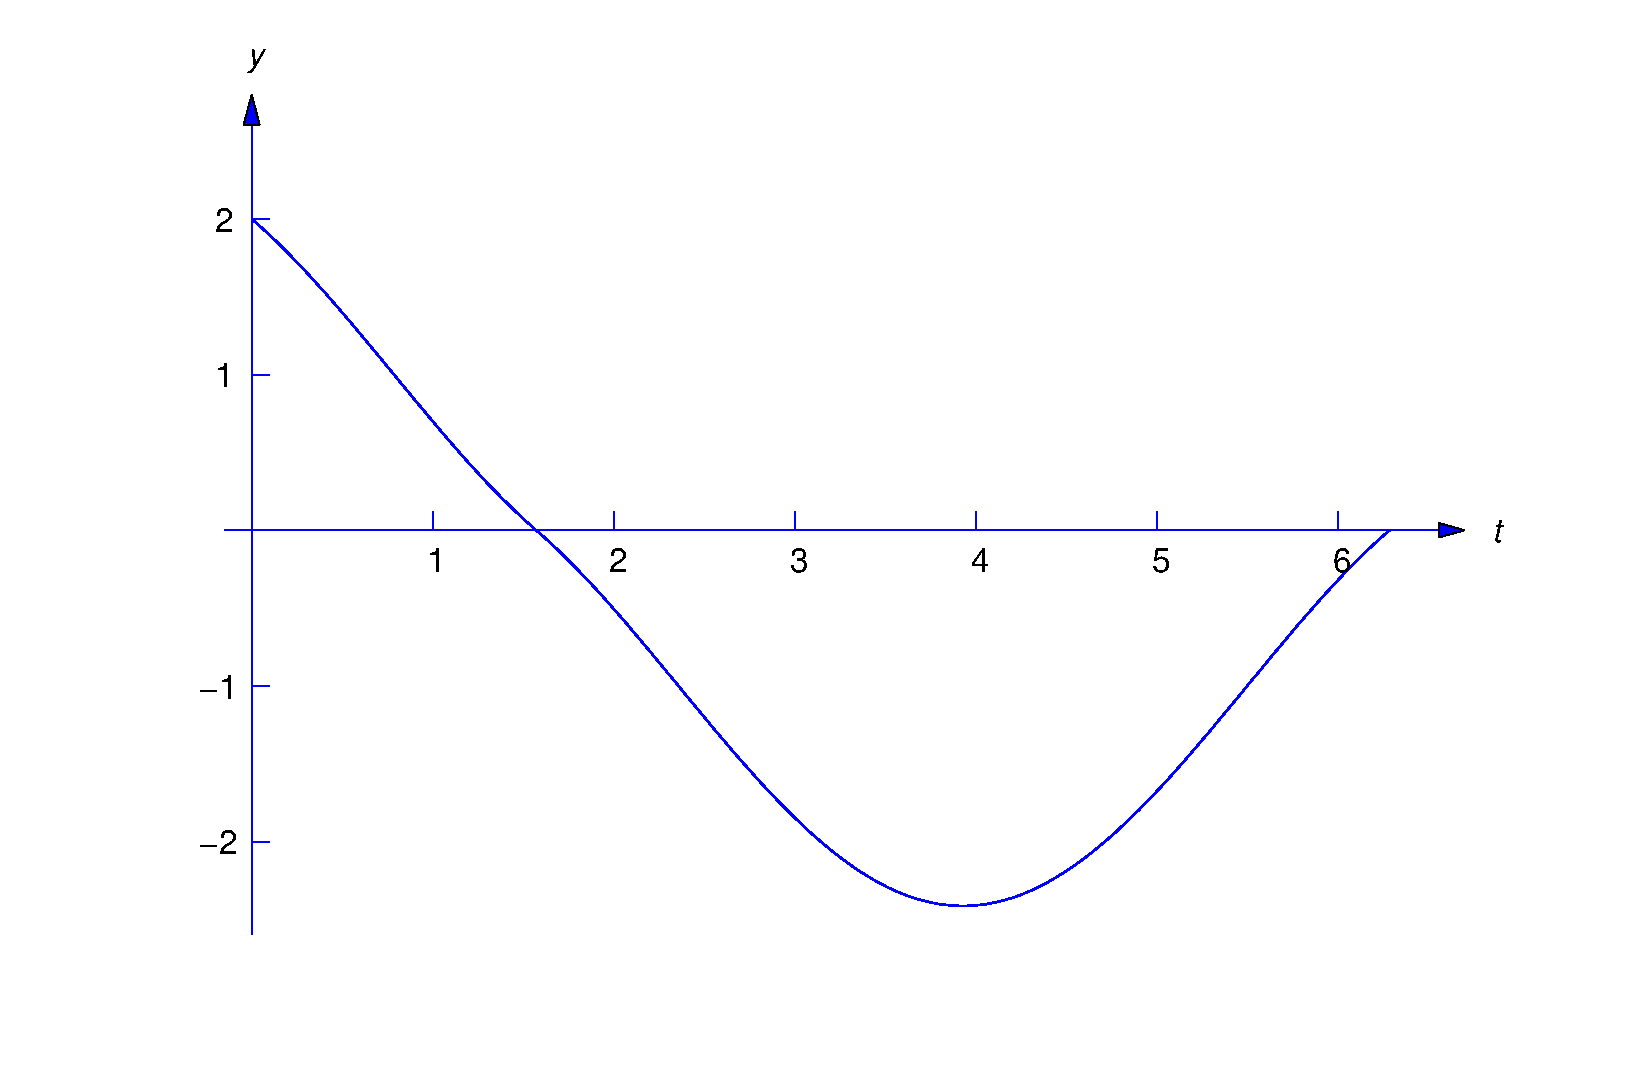
\includegraphics[bb=-78 148 689 643,width=5.67in,height=3.66in,keepaspectratio]{fig080501}
  \caption{ Graph of \eqref{eq:8.5.4}}
  \label{figure:8.5.1}
\end{figure}

If $f_0$ and $f_1$ are defined on $[0,\infty)$, we can rewrite
\eqref{eq:8.5.2} as
$$
ay''+by'+cy=f_0(t)+u(t-t_1)\left(f_1(t)-f_0(t)\right), \quad  y(0)=k_0,\quad y'(0)=k_1,
$$
and apply the method of Laplace transforms. We'll now solve
the problem considered in Example~\ref{example:8.5.1} by this method.

\begin{example}\label{example:8.5.2}\rm
\space Use the Laplace transform to solve the initial value problem
\begin{equation}\label{eq:8.5.5}
y''+y=f(t), \quad   y(0)=2,\;  y'(0)=-1,
\end{equation}
where
$$
f(t)=\left\{\begin{array}{cl}
\phantom{-}1,&0\le t<\dst{{\pi\over2}},\\
-1,&t\ge\dst{{\pi\over2}}.
\end{array}\right.
$$
\end{example}

\solution Here
$$
f(t)=1-2u\left(t-{\pi\over2}\right),
$$
so Theorem~\ref{thmtype:8.4.1} (with $g(t)=1$) implies that
$$
{\cal L}(f)={1-2e^{-{\pi s/2}}\over s}.
$$
Therefore, transforming  \eqref{eq:8.5.5} yields
$$
(s^2+1)Y(s)={1-2e^{-{\pi s/ 2}}\over s}-1+2s,
$$
 so
\begin{equation}\label{eq:8.5.6}
Y(s)=(1-2e^{-{\pi s/ 2}}) G(s)+{2s-1\over s^2+1},
\end{equation}
with
$$
G(s)={1\over s(s^2+1)}.
$$
The  form for the partial fraction expansion of $G$ is
\begin{equation}\label{eq:8.5.7}
{1\over s(s^2+1)}={A\over s}+{Bs+C\over s^2+1}.
\end{equation}
Multiplying through by $s(s^2+1)$ yields
$$
A(s^2+1)+(Bs+C)s=1,
$$
or
$$
(A+B)s^2+Cs+A=1.
$$
Equating coefficients of like powers of $s$ on the two sides of this
equation shows that $A=1$, $B=-A=-1$ and $C=0$. Hence, from
\eqref{eq:8.5.7},
$$
G(s)={1\over s}-{s\over s^2+1}.
$$
Therefore
$$
g(t)=1-\cos t.
$$
From this,  \eqref{eq:8.5.6}, and
Theorem~\ref{thmtype:8.4.2},
$$
y=1-\cos t-2u\left(t-{\pi\over2}\right)\left(1-\cos\left(t-{\pi
\over2}\right)\right)+2\cos t-\sin t.
$$
Simplifying this (recalling that $\cos (t-\pi/2)=\sin t)$ yields
$$
y=1+\cos t-\sin t-2u\left(t-{\pi\over2}\right)(1-\sin t),
$$
or
$$
y=\left\{\begin{array}{cl}
\phantom{-} 1+\cos t-\sin t,&0\le t<\dst{{\pi\over2}},\\
-1+\cos t+\sin t,&t\ge\dst{{\pi\over2}},
\end{array}\right.
$$
which is the result obtained in Example~\ref{example:8.5.1}.

\medskip
\color{blue}
\remark{It isn't obvious that using the Laplace transform to solve
\eqref{eq:8.5.2} as we did in Example~\ref{example:8.5.2} yields a function
$y$ with the properties stated in Theorem~\ref{thmtype:8.5.1}; that is,
such that $y$ and $y'$ are continuous on $[0,\infty)$ and $y''$ has
limits from the right and left at $t_1$. However, this is
true if  $f_0$ and $f_1$ are continuous and of exponential order on
$[0,\infty)$. A proof  is sketched in
Exercises~8.6.~\hspace*{-3pt}\ref{exer:8.6.11}--8.6.\hspace*{-3pt}\ref{exer:8.6.13}.}
\color{black}

\begin{example}\label{example:8.5.3}\rm
\space Solve the initial value problem
\begin{equation}\label{eq:8.5.8}
y''-y=f(t), \quad   y(0)=-1,\;  y'(0)=2,
\end{equation}
where
$$
f(t)=\left\{\begin{array}{cl}
t,&0\le t<1,\\
1,&t\ge 1.
\end{array}\right.
$$
\end{example}

\solution  Here
$$
f(t)=t-u(t-1)(t-1),
$$
so
\begin{eqnarray*}
{\cal L}(f)&=&{\cal L}(t)-{\cal L}\left(u(t-1)(t-1)\right)\\[1\jot]
&=&{\cal L}(t)-e^{-s}{\cal L}(t)\mbox{ (from
Theorem~\ref{thmtype:8.4.1})}\\[1\jot]
&=&{1\over s^2}-{e^{-s}\over s^2}.
\end{eqnarray*}
Since transforming  \eqref{eq:8.5.8} yields
$$
(s^2-1) Y(s)={\cal L}(f)+2-s,
$$
we see that
\begin{equation}\label{eq:8.5.9}
Y(s)=(1-e^{-s})H(s)+{2-s\over s^2-1},
\end{equation}
where
$$
H(s)={1\over s^2(s^2-1)}={1\over s^2-1}-{1\over s^2};
$$
 therefore
\begin{equation}\label{eq:8.5.10}
h(t)=\sinh t-t.
\end{equation}
Since
$$
{\cal L}^{-1}\left({2-s\over s^2-1}\right)=2\sinh t-\cosh t,
$$
we conclude from  \eqref{eq:8.5.9},  \eqref{eq:8.5.10}, and
Theorem~\ref{thmtype:8.4.1} that
$$
y=\sinh t-t-u(t-1)\left(\sinh (t-1)-t+1\right)+2\sinh t-
\cosh t,
$$
or
\begin{equation}\label{eq:8.5.11}
y=3\sinh t-\cosh t-t-u(t-1)\left(\sinh (t-1)-t+1\right)
\end{equation}
We leave it to you to verify that $y$  and $y'$ are continuous and
$y''$ has limits from the right and left at
$t_1=1$.

\begin{example}\label{example:8.5.4}\rm
 Solve the initial value problem
\begin{equation}\label{eq:8.5.12}
y''+y=f(t), \quad   y(0)=0,\;  y'(0)=0,
\end{equation}
where
$$
f(t)=\left\{\begin{array}{cl}
 0,&0\le t<\dst{{\pi\over4}},\\[2\jot]
\cos2t,&\dst{{\pi\over4}}\le t<\pi,\\[2\jot]
 0,&t\ge\pi.
\end{array}\right.
$$
\end{example}

\solution  Here
$$
f(t)=u(t-\pi/4)\cos2t-u(t-\pi)\cos2t,
$$
so
\begin{eqnarray*}
{\cal L}(f)&=&{\cal L}\left(u(t-\pi/4)\cos2t\right)-{\cal L}\left(
u(t-\pi)\cos2t\right)\\[1\jot]
&=&e^{-{\pi s/4}}{\cal L}\left(\cos2(t+\pi/4)\right)-e^{-\pi s}
{\cal L}\left(\cos2(t+\pi)\right)\\[1\jot]
&=&-e^{-{\pi s/4}}{\cal L}(\sin2t)-e^{-\pi s}
{\cal L}(\cos2t)\\[1\jot]
&=&-{2e^{-{\pi s/ 4}}\over s^2+4}-{se^{-\pi s}\over s^2+4}.
\end{eqnarray*}
Since transforming  \eqref{eq:8.5.12} yields
$$
(s^2+1)Y(s)={\cal L}(f),
$$
we see that
\begin{equation}\label{eq:8.5.13}
Y(s)=e^{-{\pi s/ 4}} H_1(s)+e^{-\pi s} H_2(s),
\end{equation}
where
\begin{equation}\label{eq:8.5.14}
H_1(s)=-{2\over (s^2+1)(s^2+4)}\quad\mbox{ and }\quad H_2(s)=-{s
\over
(s^2+1)(s^2+4)}.
\end{equation}
To simplify the required partial fraction expansions, we first write
$$
{1\over (x+1)(x+4)}={1\over3}\left[{1\over x+1}-{1\over
x+4}\right].
$$
Setting $x=s^2$ and substituting the result in  \eqref{eq:8.5.14} yields
$$
H_1(s)=-{2\over3}\left[{1\over s^2+1}-{1\over s^2+4}\right]
\quad\mbox{ and }\quad
H_2(s)=-{1\over3}\left[{s\over s^2+1}-{s\over s^2+4}\right].
$$
The inverse transforms are
$$
h_1(t)=-{2\over3}\sin t+{1\over3}\sin2t
\quad\mbox{ and }\;
h_2(t)=-{1\over3}\cos t+{1\over3}\cos2t.
$$
From  \eqref{eq:8.5.13} and Theorem~8.4.2,
\begin{equation}\label{eq:8.5.15}
y=u\left(t-{\pi\over4}\right) h_1\left(t-{\pi\over4}\right)+
u(t-\pi) h_2(t-\pi).
\end{equation}
Since
\begin{eqnarray*}
h_1\left(t-{\pi\over4}\right)&=&-{2\over3}\sin\left(t-{\pi\over
4}\right)+{1\over3}\sin2\left(t-{\pi\over4}\right)\\
&=&-{\sqrt{2}\over3} (\sin t-\cos t)-{1\over3}\cos2t
\end{eqnarray*}
and
\begin{eqnarray*}
h_2(t-\pi)&=&-{1\over3}\cos (t-\pi)+{1\over3}\cos2(t-\pi)\\
&=&{1\over3}\cos t+{1\over3}\cos2t,
\end{eqnarray*}
 \eqref{eq:8.5.15} can be rewritten as
$$
y=-{1\over3}u\left(t-{\pi\over4}\right)\left(\sqrt{2}(\sin
t-\cos t)+\cos2t\right)
+ {1\over3} u(t-\pi) (\cos t+\cos2t)
$$
or
\begin{equation}\label{eq:8.5.16}
y=\left\{\begin{array}{cl}
0,&0\le t<\dst{{\pi\over4}},\\[2\jot]
-\dst{{\sqrt{2}\over3}}(\sin t-\cos t)-\dst{{1\over
3}}\cos2t,&\dst{\pi\over4}\le t<\pi,\\[2\jot]
-\dst{ {\sqrt{2}\over3}}\sin t+
\dst{{1+\sqrt{2}\over3}}\cos t ,&t\ge\pi.
\end{array}\right.
\end{equation}
We leave it to you to verify that $y$ and $y'$ are continuous and
$y''$ has limits from the right and left at $t_1=\pi/4$ and $t_2=\pi$
(Figure~\ref{figure:8.5.2}).

\begin{figure}[tbp]
  \centering\color{blue}
  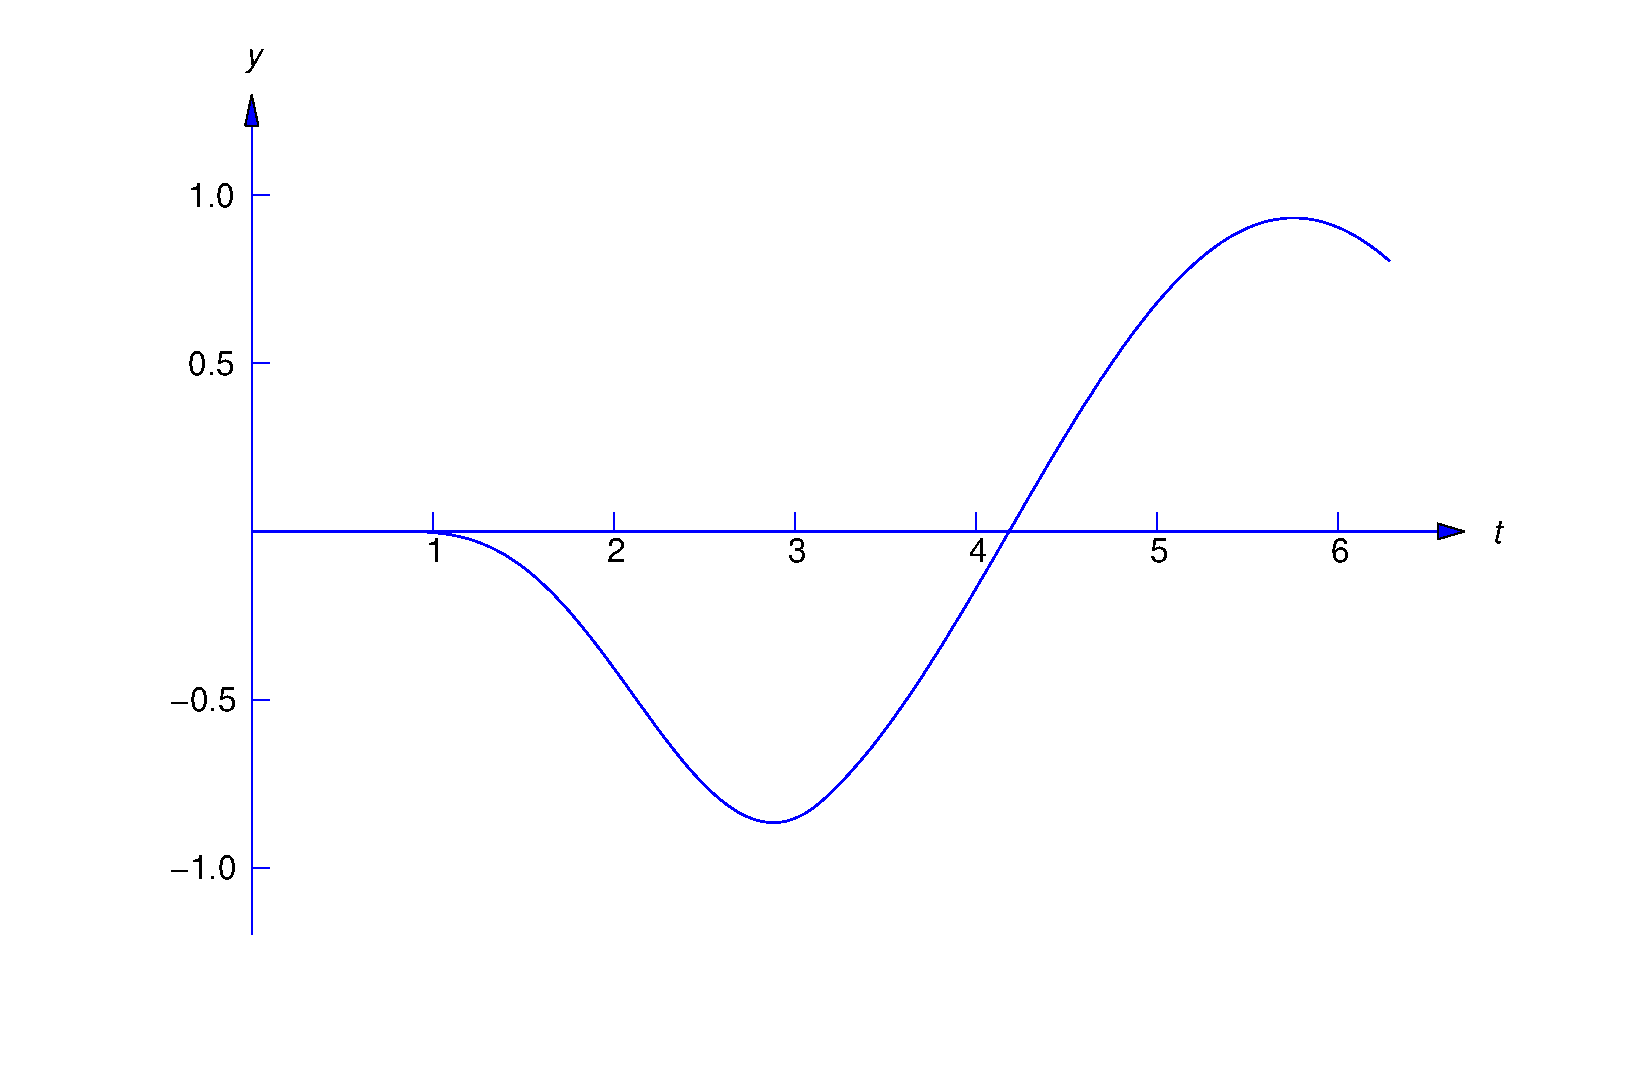
\includegraphics[bb=-78 148 689 643,width=5.67in,height=3.66in,keepaspectratio]{fig080502}
  \caption{ Graph of \eqref{eq:8.5.16}}
  \label{figure:8.5.2}
\end{figure}

\exercises
\noindent In Exercises~\ref{exer:8.5.1}--\ref{exer:8.5.20} use the Laplace
transform to solve the initial value problem.
Where indicated by\\ \CGex, graph the solution.

\begin{exerciselist}

\item\label{exer:8.5.1} $\dst{y''+y=\left\{\begin{array}{cl} 3,& 0\le
t<\pi,\\[2\jot] 0,&t\ge\pi,\end{array}\right.\qquad y(0)=0, \quad  y'(0)=0}$

\item\label{exer:8.5.2} $\dst{y''+y=\left\{\begin{array}{cl} 3,&0\le
t<4,\\; 2t-5,&t > 4,\end{array}\right.\qquad y(0)=1,\quad y'(0)=0}$

\item\label{exer:8.5.3} $\dst{y''-2y'= \left\{\begin{array}{cl} 4,&0\le
t<1,\\[2\jot] 6,&t\ge 1,\end{array}\right.\qquad y(0)=-6,\quad y'(0)=1 }$

\item\label{exer:8.5.4} $\dst{y''-y=\left\{\begin{array}{cl} e^{2t},&0\le
t< 2,\\[2\jot] 1,&t\ge 2,\end{array}\right.\qquad y(0)=3,\quad y'(0)=-1
}$

\item\label{exer:8.5.5} $\dst{y''-3y'+2y= \left\{\begin{array}{rl} 0,&0\le
t<1,\\[2\jot] 1,&1\le t<2,\\[2\jot]-1,&t\ge 2,
\end{array}\right.\qquad y(0)=-3,\quad y'(0)=1}$

\item\label{exer:8.5.6} \CGex $\dst{y''+4y= \left\{\begin{array}{cl}|\sin
t|,&0\le t<2\pi,\\[2\jot] 0,&t\ge 2\pi,\end{array}\right.\qquad
y(0)=-3,\quad y'(0)=1}$

\item\label{exer:8.5.7} $\dst{y''-5y'+4y= \left\{\begin{array}{rl} 1,&0\le
t<1\\[2\jot] -1,&1\le t<2,\\[2\jot] 0,&t\ge 2,\end{array}\right.\qquad
y(0)=3,\quad y'(0)=-5}$

\item\label{exer:8.5.8} $\dst{y''+9y= \left\{\begin{array}{cl} \cos
t,&0\le t<\dst{{3\pi\over2}},\\[2\jot] \sin
t,&t\ge\dst{{3\pi\over2}},\end{array}\right.\qquad y(0)=0,\;  y'(0)=0}$

\item\label{exer:8.5.9} \CGex $\dst{y''+4y= \left\{\begin{array}{cl} t,&0\le
t<\dst{\pi \over2},\\[2\jot]\pi,&t\ge\dst{ {\pi\over2}},
\end{array}\right.\quad y(0)=0,\quad y'(0)=0}$

\item\label{exer:8.5.10}
$\dst{y''+y=\left\{\begin{array}{cl}\phantom{-}t,&0\le t<\pi,
\\[2\jot]-t,&t\ge\pi ,\end{array}\right.\;  y(0)=0,\;  y'(0)=0}$

\item\label{exer:8.5.11} $\dst{y''-3y'+2y=\left\{\begin{array}{cl} 0,&0\le
t<2,\\2t-4,&t\ge 2,\end{array}\right. ,\quad y(0)=0,\quad y'(0)=0}$

\item\label{exer:8.5.12} $\dst{y''+y=\left\{\begin{array}{cl} t,&0\le
t<2\pi,\\-2t,&t\ge 2\pi,\end{array}\right.\quad y(0)=1,\quad y'(0)=2}$

\item\label{exer:8.5.13} \CGex
$\dst{y''+3y'+2y=\left\{\begin{array}{cl}\phantom{-}1,&0\le
t<2,\\-1,&t\ge 2,\end{array}\right.\;  y(0)=0,\;  y'(0)=0}$

\item\label{exer:8.5.14} $\dst{y''-4y'+3y=\left\{\begin{array}{cl}-1,&0\le
t<1,\\\phantom{-}1,&t\ge 1,\end{array}\right.\;  y(0)=0,\;  y'(0)=0}$

\item\label{exer:8.5.15} $\dst{y''+2y'+y=\left\{\begin{array}{cl}
e^t,&0\le t<1,\\e^t-1,&t\ge 1,\end{array}\right.\;  y(0)=3,\;
y'(0)=-1}$

\item\label{exer:8.5.16}
 $\dst{y''+2y'+y=\left\{\begin{array}{cl}
4e^t,&0\le t<1,\\0,&t\ge 1,\end{array}\right.\;  y(0)=0,\;
y'(0)=0}$

\item\label{exer:8.5.17} $\dst{y''+3y'+2y=\left\{\begin{array}{cl}
e^{-t},&0\le t<1,\\0,&t\ge 1,\end{array}\right.\;  y(0)=1,\;  y'(0)=-1}$

\item\label{exer:8.5.18} $\dst{y''-4y'+4y=\left\{\begin{array}{rl}
e^{2t},&0\le t<2,\\-e^{2t},&t\ge 2,\end{array}\right.\;  y(0)=0,\;
y'(0)=-1}$

\item\label{exer:8.5.19} \CGex $\dst{y''=\left\{\begin{array}{cl}t^2,&0\le
t<1,\\-t,&1\le t<2,\\t+1,&t\ge 2,\end{array}\right.\;  y(0)=1,\;
y'(0)=0}$

\item\label{exer:8.5.20} $\dst{y''+2y'+2y=\left\{\begin{array}{rl}1,&0\le
t<2\pi,\\t,&2\pi\le t<3\pi,\\-1,&t\ge 3\pi,\end{array}\right.\;
y(0)=2,\quad y'(0)=-1}$

\item\label{exer:8.5.21} Solve the initial value problem $$ y''=f(t), \quad
y(0)=0,\quad  y'(0)=0, $$ where $$ f(t)=m+1,\quad m\le t<m+1,\quad
m=0,1,2,\dots. $$

\item\label{exer:8.5.22} Solve the given initial value problem and find a
formula that does not involve step functions and represents $y$ on
each interval of continuity of $f$.
\begin{alist}
\item % (a)
$y''+y=f(t), \quad  y(0)=0,\quad  y'(0)=0$;

$f(t)=m+1,\quad  m\pi\le t<(m+1)\pi,\quad m=0,1,2,\dots$.

\item % (b)
$y''+y=f(t), \quad  y(0)=0,\quad y'(0)=0$;

$f(t)=(m+1)t, \quad   2m\pi\le t<2(m+1)\pi,\quad m=0,1,2,\dots$
\hint{You'll need the formula}
$$
1+2+\cdots+m={m(m+1)\over2}.
$$

\item % (c)
$y''+y=f(t), \quad  y(0)=0,\quad  y'(0)=0$;

$f(t)=(-1)^m,\quad  m\pi\le t<(m+1)\pi,\quad m=0,1,2,\dots.$

\item % (d)
$y''-y=f(t), \quad  y(0)=0,\quad  y'(0)=0$;

$f(t)=m+1,\quad  m\le t<(m+1),\quad m=0,1,2,\dots.$

\hint{You will need the formula
$$
1+r+\cdots+r^m={1-r^{m+1}\over1-r}\; (r\ne1).
$$}

\item % (d)
$y''+2y'+2y=f(t), \quad  y(0)=0,\quad  y'(0)=0$;

$f(t)=(m+1)(\sin t+2\cos t),\quad  2m\pi\le t<2(m+1)\pi,\quad
m=0,1,2,\dots.$

(See the hint in \part{d}.)

\item % (f)
$y''-3y'+2y=f(t), \quad  y(0)=0,\quad y'(0)=0$;

$f(t)=m+1,\quad  m\le t<m+1,\quad m=0,1,2,\dots.$

 (See the hints in \part{b} and \part{d}.)
\end{alist}

\item\label{exer:8.5.23}
\begin{alist}
\item % (a)
Let $g$ be  continuous on  $(\alpha,\beta)$
 and differentiable on the  $(\alpha,t_0)$
and $(t_0,\beta)$. Suppose $A=\lim_{t\to t_0-}g'(t)$
and $B=\lim_{t\to t_0+}g'(t)$ both exist. Use the mean value theorem
to show that
$$
\lim_{t\to t_0-}{g(t)-g(t_0)\over t-t_0}=A\quad\mbox{ and }\quad
\lim_{t\to t_0+}{g(t)-g(t_0)\over t-t_0}=B.
$$
\item % (b)
Conclude from \part{a} that $g'(t_0)$ exists and $g'$ is continuous at
$t_0$ if $A=B$.

\item % (c)
Conclude from \part{a}
 that if $g$  is differentiable on $(\alpha,\beta)$ then
$g'$ can't have a jump discontinuity on $(\alpha,\beta)$.
\end{alist}

\item\label{exer:8.5.24}
\begin{alist}
\item % (a)
Let $a$, $b$, and $c$ be constants, with $a\ne0$. Let $f$ be piecewise
continuous on an interval $(\alpha,\beta)$, with a single jump
discontinuity at a point $t_0$ in $(\alpha,\beta)$. Suppose $y$
and $y'$ are continuous on $(\alpha,\beta)$ and $y''$ on
$(\alpha,t_0)$ and $(t_0,\beta)$. Suppose  also that
$$
ay''+by'+cy=f(t)
\eqno{\rm (A)}
$$
on $(\alpha,t_0)$ and $(t_0,\beta)$.
Show that
$$
y''(t_0+)-y''(t_0-)={f(t_0+)-f(t_0-)\over a}\ne0.
$$
\item % (b)
Use \part{a}  and Exercise~\ref{exer:8.5.23}\part{c} to show that
(A)
does not  have  solutions on any interval $(\alpha,\beta)$ that contains
a jump discontinuity of $f$.
\end{alist}

\item\label{exer:8.5.25}
Suppose $P_0,P_1$, and $P_2$ are continuous and $P_0$
has no zeros on an open interval $(a,b)$, and  that $F$
has a jump discontinuity at a point $t_0$ in $(a,b)$.
Show that the differential equation
$$
P_0(t)y''+P_1(t)y'+P_2(t)y=F(t)
$$
has no solutions on $(a,b)$.\hint{Generalize the result of
Exercise~$\ref{exer:8.5.24}$ and use Exercise~$\ref{exer:8.5.23}\part{c}$.}

\item\label{exer:8.5.26}
Let $0=t_0<t_1<\cdots <t_n$. Suppose $f_m$ is continuous
on $[t_m,\infty)$ for $m=1,\dots,n$.
 Let
$$
f(t)=
\left\{\begin{array}{cl}
f_m(t),&t_m\le t< t_{m+1},\quad m=1,\dots,n-1,\\
f_n(t),&t\ge t_n.
\end{array}\right.
$$
Show that the
solution of
$$
ay''+by'+cy=f(t), \quad  y(0)=k_0,\quad y'(0)=k_1,
$$
as defined following  Theorem~8.5.1, is given by
$$
y=\left\{\begin{array}{cl}
 z_0(t),&0\le t<t_1,\\[1\jot]
z_0(t)+ z_1(t),&t_1\le t<t_2,\\
&\vdots\\
z_0+\cdots+z_{n-1}(t),&t_{n-1}\le t<t_n,\\[1\jot]
z_0+\cdots+ z_n(t),&t\ge t_n,
\end{array}\right.
$$
where $z_0$ is the solution of
$$
az''+bz'+cz=f_0(t), \quad  z(0)=k_0,\quad  z'(0)=k_1
$$
and $z_m$ is the solution of
$$
az''+bz'+cz=f_m(t)-f_{m-1}(t), \quad  z(t_m)=0,\quad z'(t_m)=0
$$
for $m=1,\dots,n$.
\end{exerciselist}


\section{Convolution}

\noindent
In this section we consider the problem of finding the inverse Laplace transform of a product
$H(s)=F(s)G(s)$, where $F$ and $G$ are the Laplace transforms of known functions $f$ and $g$. To
motivate our interest in this problem, consider the initial value problem
\[
  ay''+by'+cy=f(t),\quad y(0)=0,\quad y'(0)=0.
\]
Taking Laplace transforms yields
\[
  (as^{2}+bs+c)Y(s)=F(s),
\]
so
\begin{equation}
  \label{eq:8.6.1}Y(s)=F(s)G(s),
\end{equation}
where
\[
  G(s)=\frac{1}{as^{2}+bs+c}.
\]

Until now we haven't been interested in the factorization indicated in \eqref{eq:8.6.1}, since we
dealt only with differential equations with specific forcing functions. Hence, we could simply do
the indicated multiplication in \eqref{eq:8.6.1} and use the table of Laplace transforms to find
$y={\cal L}^{-1}(Y)$. However, this isn't possible if we want a {\color{blue}\it formula} for $y$ in
terms of $f$, which may be unspecified.

To motivate the formula for ${\cal L}^{-1}(FG)$, consider the initial value problem
\begin{equation}
  \label{eq:8.6.2}y'-ay=f(t),\quad y(0)=0,
\end{equation}
which we first solve without using the Laplace transform. The solution of the differential equation
in \eqref{eq:8.6.2} is of the form $y=ue^{at}$ where
\[
  u'=e^{-at}f(t).
\]
Integrating this from $0$ to $t$ and imposing the initial condition $u(0)=y(0)=0$ yields
\[
  u=\int_{0}^{t}e^{-a\tau}f(\tau)\,d\tau.
\]
Therefore
\begin{equation}
  \label{eq:8.6.3}y(t)=e^{at}\int_{0}^{t}e^{-a\tau}f(\tau)\,d\tau=\int_{0}^{t}e^{a(t-\tau)}f(\tau)\,d\tau.
\end{equation}

Now we'll use the Laplace transform to solve \eqref{eq:8.6.2} and compare the result to
\eqref{eq:8.6.3}. Taking Laplace transforms in \eqref{eq:8.6.2} yields
\[
  (s-a)Y(s)=F(s),
\]
so
\[
  Y(s)=F(s)\frac{1}{s-a},
\]
which implies that
\begin{equation}
  \label{eq:8.6.4}y(t)={\cal L}^{-1}\left(F(s)\frac{1}{s-a}\right).
\end{equation}
If we now let $g(t)=e^{at}$, so that
\[
  G(s)=\frac{1}{s-a},
\]
then \eqref{eq:8.6.3} and \eqref{eq:8.6.4} can be written as
\[
  y(t)=\int_{0}^{t}f(\tau)g(t-\tau)\,d\tau
\]
and
\[
  y={\cal L}^{-1}(FG),
\]
respectively. Therefore
\begin{equation}
  \label{eq:8.6.5}{\cal L}^{-1}(FG)=\int_{0}^{t}f(\tau)g(t-\tau)\,d\tau
\end{equation}
in this case.

This motivates the next definition.

\begin{definition}
  \color{blue}
  \label{thmtype:8.6.1} \rm The {\color{blue}\it convolution\/} $f*g$ of two functions $f$ and $g$
  is defined by
  \[
    (f*g)(t)=\int_{0}^{t}f(\tau)g(t-\tau)\,d\tau.
  \]
\end{definition}

It can be shown (Exercise~\ref{exer:8.6.6}) that $f\ast g=g\ast f$; that is,
\[
  \int_{0}^{t}f(t-\tau)g(\tau)\,d\tau=\int_{0}^{t}f(\tau)g(t-\tau)\,d\tau.
\]

Eqn.~\eqref{eq:8.6.5} shows that ${\cal L}^{-1}(FG)=f*g$ in the special case where $g(t)=e^{at}$.
This next theorem states that this is true in general.

\begin{theorem}
  \color{blue}
  $[$The Convolution Theorem$]$\label{thmtype:8.6.2} Suppose $f$ and $g$ are piecewise continuous on $[0,\infty)$ and their Laplace transforms converge absolutely at $s$. If ${\cal L}(f)=F$ and ${\cal L}(g)=G$, then
  \[
    {\cal L}(f*g)=FG.
  \]
\end{theorem}

A complete proof of the convolution theorem is beyond the scope of this book. However, we'll verify the conclusion of the theorem in a purely
computational way. By the definition of the Laplace transform,
\[
  {\cal L}(f\ast g)=\int_{0}^{\infty}e^{-st}(f\ast g)(t)\,dt=\int_{0}^{\infty}e^{-st}\int_{0}^{t}f(\tau)g(t-\tau)\,d\tau\,dt.
\]
This iterated integral equals a double integral over the region shown in Figure~\ref{figure:8.6.1}.
Reversing the order of integration yields
\begin{equation}
  \label{eq:8.6.6}{\cal L}(f*g)=\int_{0}^{\infty}f(\tau)\int^{\infty}_{\tau}e^{-st}g(t-\tau)\, dt \,d\tau.
\end{equation}
However, the substitution $x=t-\tau$ shows that
\begin{eqnarray*}
  \int^{\infty}_{\tau}e^{-st}g(t-\tau)\,dt & = & \int_{0}^{\infty}e^{-s(x+\tau)}g(x)\,dx \\
                                           & = & e^{-s\tau}\int_{0}^{\infty}e^{-sx}g(x)\,dx=e^{-s\tau}G(s).
\end{eqnarray*}
Substituting this into \eqref{eq:8.6.6} and noting that $G(s)$ is independent of $\tau$ yields
\begin{eqnarray*}
  {\cal L}(f\ast g) & = & \int_{0}^{\infty}e^{-s\tau}f(\tau)G(s)\,d\tau \\
                    & = & G(s)\int_{0}^{\infty}e^{-s\tau}f(\tau)\,d\tau=F(s)G(s).
\end{eqnarray*}

\

\begin{figure}[tbp]
  \centering
  \color{blue}
  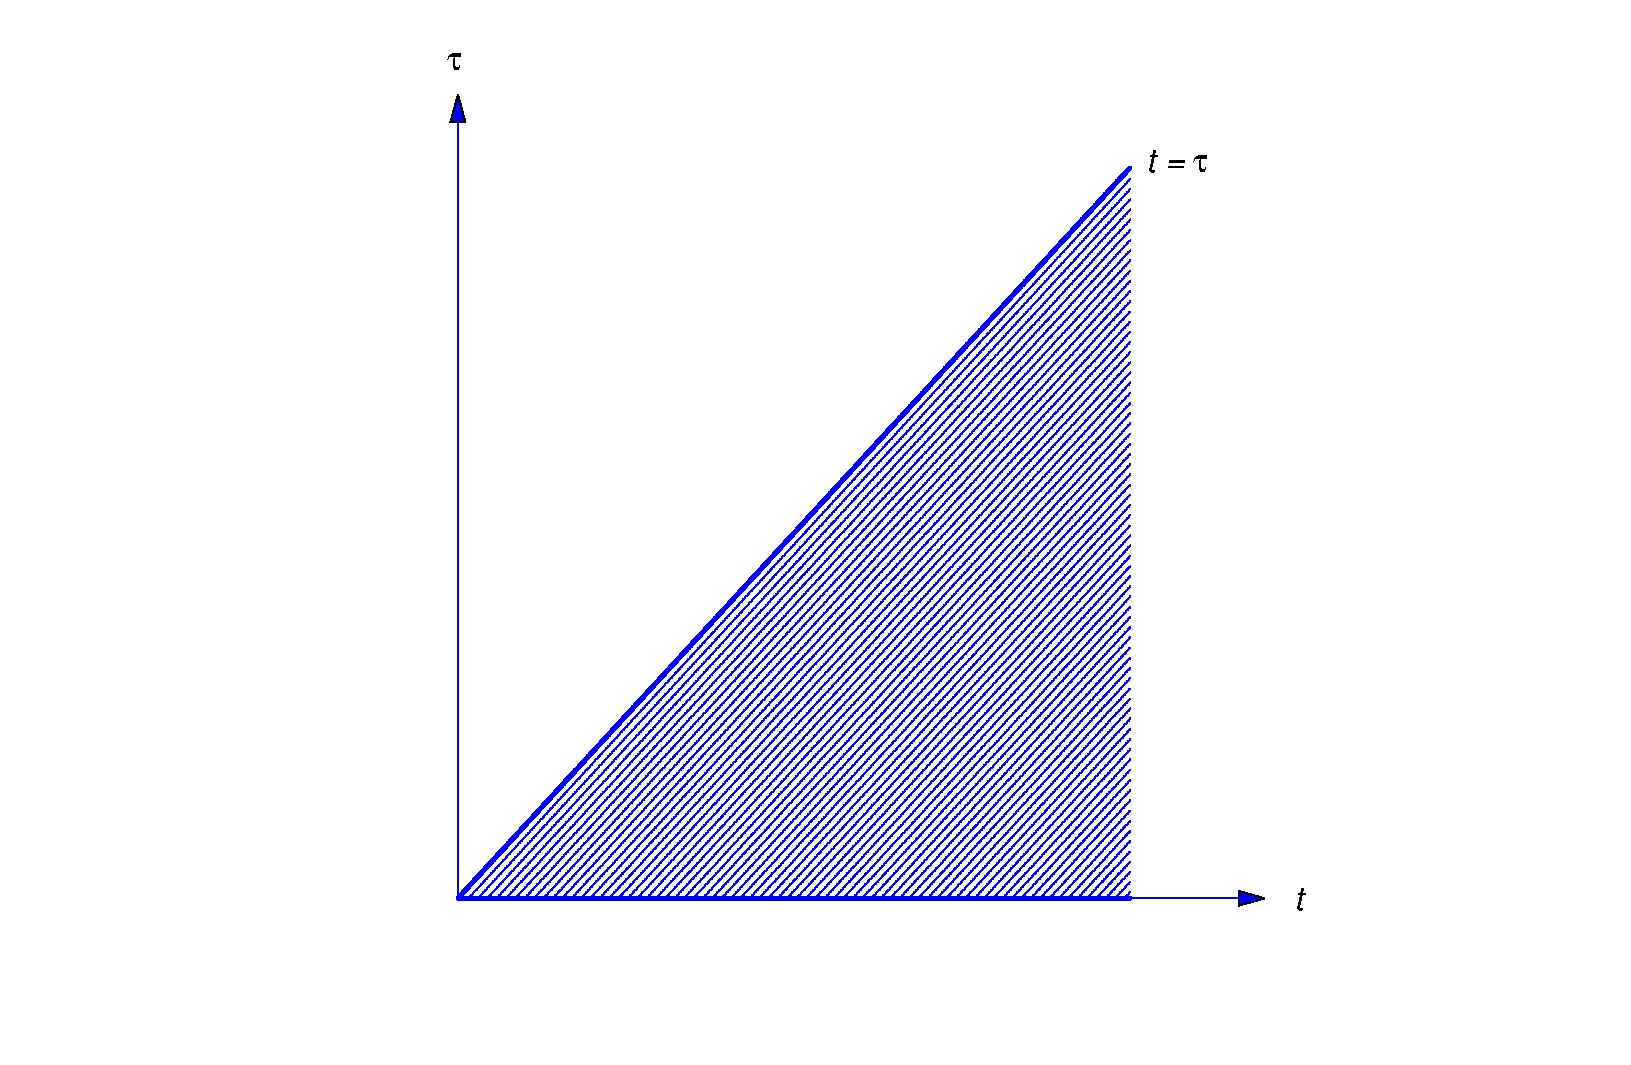
\includegraphics[bb=-78 148 689 643, width=5.67in, height=3.66in, keepaspectratio]{fig080601}
  \caption{The region of integration for the convolution theorem}
  \label{figure:8.6.1}
\end{figure}

\begin{example}
  \label{example:8.6.1}\rm Let
  \[
    f(t)=e^{at}\mbox{\quad and \quad}g(t)=e^{bt}\qquad(a\ne b).
  \]
  Verify that ${\cal L}(f\ast g)={\cal L}(f){\cal L}(g)$, as implied by the convolution theorem.
\end{example}

\solution We first compute
\[
  \begin{array}{ccccc}
    (f\ast g)(t) & = & \dst\int_{0}^{t}e^{a\tau}e^{b(t-\tau)}\,d\tau         & = & \dst e^{bt}\int_{0}^{t}e^{(a-b)\tau}d\tau       \\[2\jot]
                 & = & \dst{e^{bt}\frac{e^{(a-b)\tau}}{a-b}\,\bigg|^{t}_{0}} & = & \dst\frac{e^{bt}\left[e^{(a-b)t}-1\right]}{a-b} \\[2\jot]
                 & = & \dst\frac{e^{at}-e^{bt}}{a-b}.
  \end{array}
\]
Since
\[
  e^{at}\leftrightarrow\frac{1}{s-a}\quad\mbox{ and }\quad e^{bt}\leftrightarrow\frac{1}{s-b},
\]
it follows that
\begin{eqnarray*}
  {\cal L}(f\ast g) & = & \frac{1}{a-b}\left[\frac{1}{s-a}-\frac{1}{s-b}\right] \\[10pt]
                    & = & \frac{1}{(s-a)(s-b)}                                  \\[2\jot]
                    & = & {\cal L}(e^{at}){\cal L}(e^{bt})={\cal L}(f){\cal L}(g).
\end{eqnarray*}

\boxit{A Formula for the Solution of an Initial Value Problem}

\noindent
The convolution theorem provides a formula for the solution of an initial value problem for a linear
constant coefficient second order equation with an unspecified forcing function. The next three examples illustrate
this.

\begin{example}
  \label{example:8.6.2}\rm Find a formula for the solution of the initial value problem
  \begin{equation}
    \label{eq:8.6.7}y''-2y'+y=f(t),\quad y(0)=k_{0},\quad y'(0)=k_{1}.
  \end{equation}
\end{example}

\solution Taking Laplace transforms in \eqref{eq:8.6.7} yields
\[
  (s^{2}-2s+1)Y(s)=F(s)+(k_{1}+k_{0}s)-2k_{0}.
\]
Therefore
\begin{eqnarray*}
  Y(s) & = & \frac{1}{(s-1)^{2}}F(s)+\frac{k_{1}+k_{0}s-2k_{0}}{(s-1)^{2}} \\[2\jot]
       & = & \frac{1}{(s-1)^{2}}F(s)+\frac{k_{0}}{s-1}+\frac{k_{1}-k_{0}}{(s-1)^{2}}.
\end{eqnarray*}
From the table of Laplace transforms,
\[
  {\cal L}^{-1}\left(\frac{k_{0}}{s-1}+\frac{k_{1}-k_{0}}{(s-1)^{2}}\right) =e^{t}\left(k_{0}+(k_{1}-k_{0})t\right).
\]
Since
\[
  \frac{1}{(s-1)^{2}}\leftrightarrow te^{t}\mbox{\quad and \quad }F(s) \leftrightarrow f(t),
\]
the convolution theorem implies that
\[
  {\cal L}^{-1}\left(\frac{1}{(s-1)^{2}}F(s)\right)= \int_{0}^{t}\tau e^{\tau}f(t-\tau)\,d\tau.
\]
Therefore the solution of \eqref{eq:8.6.7} is
\[
  y(t)=e^{t}\left(k_{0}+(k_{1}-k_{0})t\right)+\int_{0}^{t}\tau e^{\tau}f(t-\tau)\, d\tau.
\]

\begin{example}
  \label{example:8.6.3}\rm Find a formula for the solution of the initial value problem
  \begin{equation}
    \label{eq:8.6.8}y''+4y=f(t),\quad y(0)=k_{0},\quad y'(0)=k_{1}.
  \end{equation}
\end{example}

\solution Taking Laplace transforms in \eqref{eq:8.6.8} yields
\[
  (s^{2}+4)Y(s)=F(s)+k_{1}+k_{0}s.
\]
Therefore
\[
  Y(s)=\frac{1}{(s^{2}+4)}F(s)+\frac{k_{1}+k_{0}s}{s^{2}+4}.
\]
From the table of Laplace transforms,
\[
  {\cal L}^{-1}\left(\frac{k_{1}+k_{0}s}{s^{2}+4}\right)=k_{0}\cos2t+\frac{k_{1}}{2}\sin2t.
\]
Since
\[
  \frac{1}{(s^{2}+4)}\leftrightarrow\frac{1}{2}\sin2t\mbox{\quad and \quad}F(s)\leftrightarrow f(t),
\]
the convolution theorem implies that
\[
  {\cal L}^{-1}\left(\frac{1}{(s^{2}+4)}F(s)\right)= \frac{1}{2}\int_{0}^{t}f(t-\tau)\sin2\tau\, d\tau.
\]
Therefore the solution of \eqref{eq:8.6.8} is
\[
  y(t)=k_{0}\cos2t+\frac{k_{1}}{2}\sin2t+\frac{1}{2}\int_{0}^{t}f(t-\tau)\sin 2\tau\,d\tau.
\]

\begin{example}
  \label{example:8.6.4}\rm Find a formula for the solution of the initial value problem
  \begin{equation}
    \label{eq:8.6.9}y''+2y'+2y=f(t),\quad y(0)=k_{0},\quad y'(0)=k_{1}.
  \end{equation}
\end{example}

\solution Taking Laplace transforms in \eqref{eq:8.6.9} yields
\[
  (s^{2}+2s+2)Y(s)=F(s)+k_{1}+k_{0}s+2k_{0}.
\]
Therefore
\begin{eqnarray*}
  Y(s) & = & \frac{1}{(s+1)^{2}+1}F(s)+\frac{k_{1}+k_{0}s+2k_{0}}{(s+1)^{2}+1} \\[2\jot]
       & = & \frac{1}{(s+1)^{2}+1}F(s)+\frac{(k_{1}+k_{0})+k_{0}(s+1)}{(s+1)^{2}+1}.
\end{eqnarray*}
From the table of Laplace transforms,
\[
  {\cal L}^{-1}\left(\frac{(k_{1}+k_{0})+k_{0}(s+1)}{(s+1)^{2}+1}\right)= e^{-t}\left((k_{1}+k_{0})\sin t+k_{0}\cos t\right).
\]
Since
\[
  \frac{1}{(s+1)^{2}+1}\leftrightarrow e^{-t}\sin t\mbox{\quad and \quad}F(s)\leftrightarrow f(t),
\]
the convolution theorem implies that
\[
  {\cal L}^{-1}\left(\frac{1}{(s+1)^{2}+1}F(s)\right)= \int_{0}^{t}f(t-\tau)e^{-\tau}\sin\tau \,d\tau.
\]
Therefore the solution of \eqref{eq:8.6.9} is
\begin{equation}
  \label{eq:8.6.10}y(t)=e^{-t}\left((k_{1}+k_{0})\sin t+k_{0}\cos t\right)+\int_{0}^{t}f(t-\tau)e^{-\tau}\sin\tau\,d\tau.
\end{equation}

\boxit{Evaluating Convolution Integrals}

\noindent
We'll say that an integral of the form $\int_{0}^{t}u(\tau)v(t-\tau)\,d\tau$ is a {\color{blue}\it
convolution integral\/}. The convolution theorem provides a convenient way to evaluate convolution
integrals.

\begin{example}
  \label{example:8.6.5}\rm Evaluate the convolution integral
  \[
    h(t)=\int_{0}^{t}(t-\tau)^{5}\tau^{7}d\tau.
  \]
\end{example}

\solution We could evaluate this integral by expanding $(t-\tau)^{5}$ in powers of $\tau$ and then
integrating. However, the convolution theorem provides an easier way. The integral is the
convolution of $f(t)=t^{5}$ and $g(t)=t^{7}$. Since
\[
  t^{5}\leftrightarrow\frac{5!}{s^{6}}\quad\mbox{ and }\quad t^{7}\leftrightarrow\frac{7!}{s^{8}},
\]
the convolution theorem implies that
\[
  h(t)\leftrightarrow\frac{5!7!}{s^{14}}=\frac{5!7!}{13!}\,\frac{13!}{s^{14}},
\]
where we have written the second equality because
\[
  \frac{13!}{s^{14}}\leftrightarrow t^{13}.
\]
Hence,
\[
  h(t)=\frac{5!7!}{13!}\,t^{13}.
\]

\begin{example}
  \label{example:8.6.6}\rm Use the convolution theorem and a partial fraction expansion to evaluate
  the convolution integral
  \[
    h(t)=\int_{0}^{t}\sin a(t-\tau)\cos b\tau\,d\tau\quad(|a|\ne|b|).
  \]
\end{example}

\solution Since
\[
  \sin at\leftrightarrow\frac{a}{s^{2}+a^{2}}\quad\mbox{and}\quad \cos bt\leftrightarrow\frac{s}{s^{2}+b^{2}},
\]
the convolution theorem implies that
\[
  H(s)=\frac{a}{s^{2}+a^{2}}\frac{s}{s^{2}+b^{2}}.
\]
Expanding this in a partial fraction expansion yields
\[
  H(s)=\frac{a}{b^{2}-a^{2}}\left[\frac{s}{s^{2}+a^{2}}-\frac{s}{s^{2}+b^{2}}\right].
\]
Therefore
\[
  h(t)=\frac{a}{b^{2}-a^{2}}\left(\cos at-\cos bt\right).
\]

\boxit{Volterra Integral Equations}

\noindent
An equation of the form
\begin{equation}
  \label{eq:8.6.11}y(t)=f(t)+\int_{0}^{t}k(t-\tau)y(\tau)\,d\tau
\end{equation}
is a
\href{https://mathshistory.st-andrews.ac.uk/Biographies/Volterra/}{\color{blue}
\it Volterra integral equation}. Here $f$ and $k$ are given functions and $y$ is unknown. Since the
integral on the right is a convolution integral, the convolution theorem provides a convenient
formula for solving \eqref{eq:8.6.11}. Taking Laplace transforms in \eqref{eq:8.6.11} yields
\[
  Y(s)=F(s)+K(s)Y(s),
\]
and solving this for $Y(s)$ yields
\[
  Y(s)=\frac{F(s)}{1-K(s)}.
\]
We then obtain the solution of \eqref{eq:8.6.11} as $y={\cal L}^{-1}(Y)$.

\begin{example}
  \label{example:8.6.7}\rm Solve the integral equation
  \begin{equation}
    \label{eq:8.6.12}y(t)=1+2\int_{0}^{t}e^{-2(t-\tau)}y(\tau)\,d\tau.
  \end{equation}
\end{example}

\solution Taking Laplace transforms in \eqref{eq:8.6.12} yields
\[
  Y(s)=\frac{1}{s}+\frac{2}{s+2}Y(s),
\]
and solving this for $Y(s)$ yields
\[
  Y(s)=\frac{1}{s}+\frac{2}{s^{2}}.
\]
Hence,
\[
  y(t)=1+2t.
\]

\boxit{Transfer Functions}

\noindent
The next theorem presents a formula for the solution of the general initial value problem
\[
  ay''+by'+cy=f(t),\quad y(0)=k_{0},\quad y'(0)=k_{1},
\]
where we assume for simplicity that $f$ is continuous on $[0,\infty)$ and that ${\cal L}(f)$ exists.
In Exercises~\ref{exer:8.6.11}--\ref{exer:8.6.14} it's shown that the formula is valid under much
weaker conditions on $f$.

\begin{theorem}
  \color{blue}
  \label{thmtype:8.6.3} Suppose $f$ is continuous on $[0,\infty)$ and has a Laplace transform. Then
  the solution of the initial value problem
  \begin{equation}
    \label{eq:8.6.13}ay''+by'+cy=f(t),\quad y(0)=k_{0},\quad y'(0)=k_{1},
  \end{equation}
  is
  \begin{equation}
    \label{eq:8.6.14}y(t)=k_{0}y_{1}(t)+k_{1}y_{2}(t)+\int_{0}^{t}w(\tau)f(t-\tau)\,d\tau,
  \end{equation}
  where $y_{1}$ and $y_{2}$ satisfy
  \begin{equation}
    \label{eq:8.6.15}ay_{1}''+by_{1}'+cy_{1}=0,\quad y_{1}(0)=1,\quad y_{1}'(0)=0,
  \end{equation}
  and
  \begin{equation}
    \label{eq:8.6.16}ay_{2}''+by_{2}'+cy_{2}=0,\quad y_{2}(0)=0,\quad y_{2}'(0)=1,
  \end{equation}
  and
  \begin{equation}
    \label{eq:8.6.17}w(t)=\frac{1}{a}y_{2}(t).
  \end{equation}
\end{theorem}

\proof Taking Laplace transforms in \eqref{eq:8.6.13} yields
\[
  p(s)Y(s)=F(s)+a(k_{1}+k_{0}s)+bk_{0},
\]
where
\[
  p(s)=as^{2}+bs+c.
\]
Hence,
\begin{equation}
  \label{eq:8.6.18}Y(s)=W(s)F(s)+V(s)
\end{equation}
with
\begin{equation}
  \label{eq:8.6.19}W(s)=\frac{1}{p(s)}
\end{equation}
and
\begin{equation}
  \label{eq:8.6.20}V(s)=\frac{a(k_{1}+k_{0}s)+bk_{0}}{p(s)}.
\end{equation}

Taking Laplace transforms in \eqref{eq:8.6.15} and \eqref{eq:8.6.16} shows that
\[
  p(s)Y_{1}(s)=as+b\quad\mbox{and}\quad p(s)Y_{2}(s)=a.
\]
Therefore
\[
  Y_{1}(s)=\frac{as+b}{p(s)}
\]
and
\begin{equation}
  \label{eq:8.6.21}Y_{2}(s)=\frac{a}{p(s)}.
\end{equation}
Hence, \eqref{eq:8.6.20} can be rewritten as
\[
  V(s)=k_{0}Y_{1}(s)+k_{1}Y_{2}(s).
\]
Substituting this into \eqref{eq:8.6.18} yields
\[
  Y(s)=k_{0}Y_{1}(s)+k_{1}Y_{2}(s)+\frac{1}{a}Y_{2}(s)F(s).
\]
Taking inverse transforms and invoking the convolution theorem yields \eqref{eq:8.6.14}. Finally,
\eqref{eq:8.6.19} and \eqref{eq:8.6.21} imply \eqref{eq:8.6.17}.\bbox

It is useful to note from \eqref{eq:8.6.14} that $y$ is of the form
\[
  y=v+h,
\]
where
\[
  v(t)=k_{0}y_{1}(t)+k_{1}y_{2}(t)
\]
depends on the initial conditions and is independent of the forcing function, while
\[
  h(t)=\int_{0}^{t}w(\tau)f(t-\tau)\, d\tau
\]
depends on the forcing function and is independent of the initial conditions. If the zeros of the
characteristic polynomial
\[
  p(s)=as^{2}+bs+c
\]
of the complementary equation have negative real parts, then $y_{1}$ and $y_{2}$ both approach zero
as $t\to\infty$, so $\lim_{t\to\infty}v(t)=0$ for any choice of initial conditions. Moreover, the
value of $h(t)$ is essentially independent of the values of $f(t-\tau)$ for large $\tau$, since
$\lim_{\tau\to\infty}w(\tau)=0$. In this case we say that $v$ and $h$ are {\color{blue}\it
transient\/} and {\color{blue}\it steady state components\/}, respectively, of the solution $y$ of
\eqref{eq:8.6.13}. These definitions apply to the initial value problem of
Example~\ref{example:8.6.4}, where the zeros of
\[
  p(s)=s^{2}+2s+2=(s+1)^{2}+1
\]
are $-1\pm i$. From \eqref{eq:8.6.10}, we see that the solution of the general initial value problem
of Example~\ref{example:8.6.4} is $y=v+h$, where
\[
  v(t)=e^{-t}\left((k_{1}+k_{0})\sin t+k_{0}\cos t\right)
\]
is the transient component of the solution and
\[
  h(t)=\int_{0}^{t}f(t-\tau)e^{-\tau}\sin\tau\,d\tau
\]
is the steady state component. The definitions don't apply to the initial value problems considered
in Examples~\ref{example:8.6.2} and \ref{example:8.6.3}, since the zeros of the characteristic
polynomials in these two examples don't have negative real parts.

In physical applications where the input $f$ and the output $y$ of a device are related by
\eqref{eq:8.6.13}, the zeros of the characteristic polynomial usually do have negative real parts.
Then $W={\cal L}(w)$ is called the {\color{blue}\it transfer function\; } of the device. Since
\[
  H(s)=W(s)F(s),
\]
we see that
\[
  W(s)=\frac{H(s)}{F(s)}
\]
is the ratio of the transform of the steady state output to the transform of the input.

Because of the form of
\[
  h(t)=\int_{0}^{t}w(\tau)f(t-\tau)\,d\tau,
\]
$w$ is sometimes called the {\color{blue}\it weighting function} of the device, since it assigns
weights to past values of the input $f$. It is also called the {\color{blue}\it impulse response} of
the device, for reasons discussed in the next section.

Formula \eqref{eq:8.6.14} is given in more detail in Exercises~\ref{exer:8.6.8}--\ref{exer:8.6.10}
for the three possible cases where the zeros of $p(s)$ are real and distinct, real and repeated, or
complex conjugates, respectively.

\exercises

\begin{exerciselist}
  \item\label{exer:8.6.1} Express the inverse transform as an integral.

  \begin{description}
    \item
      \begin{tabular}[t]{@{}p{168pt}@{}p{168pt}}
        \part{a} $\dst\frac{1}{s^{2}(s^{2}+4)}$ & \part{b} $\dst\frac{s}{(s+2)(s^{2}+9)}$
      \end{tabular}

    \item
      \begin{tabular}[t]{@{}p{168pt}@{}p{168pt}}
        \part{c} $\dst\frac{s}{(s^{2}+4)(s^{2}+9)}$ & \part{d} $\dst\frac{s}{(s^{2}+1)^{2}}$
      \end{tabular}

    \item
      \begin{tabular}[t]{@{}p{168pt}@{}p{168pt}}
        \part{e} $\dst\frac{1}{s(s-a)}$ & \part{f} $\dst\frac{1}{(s+1)(s^{2}+2s+2)}$
      \end{tabular}

    \item
      \begin{tabular}[t]{@{}p{168pt}@{}p{168pt}}
        \part{g} $\dst\frac{1}{(s+1)^{2}(s^{2}+4s+5)}$ & \part{h} $\dst\frac{1}{(s-1)^{3}(s+2)^{2}}$
      \end{tabular}

    \item
      \begin{tabular}[t]{@{}p{168pt}@{}p{168pt}}
        \part{i} $\dst\frac{s-1}{s^{2}(s^{2}-2s+2)}$ & \part{j} $\dst\frac{s(s+3)}{(s^{2}+4)(s^{2}+6s+10)}$
      \end{tabular}

    \item
      \begin{tabular}[t]{@{}p{168pt}@{}p{168pt}}
        \part{k} $\dst\frac{1}{(s-3)^{5}s^{6}}$ & \part{l} $\dst\frac{1}{(s-1)^{3}(s^{2}+4)}$
      \end{tabular}

    \item
      \begin{tabular}[t]{@{}p{168pt}@{}p{168pt}}
        \part{m} $\dst\frac{1}{s^{2}(s-2)^{3}}$ & \part{n} $\dst\frac{1}{s^{7}(s-2)^{6}}$
      \end{tabular}
  \end{description}

  \item\label{exer:8.6.2} Find the Laplace transform.

  \begin{description}
    \item
      \begin{tabular}[t]{@{}p{168pt}@{}p{168pt}}
        \part{a} $\dst{\int_{0}^{t}\sin a\tau\cos b(t-\tau)\,d\tau}$ & \part{b} $\dst{\int_{0}^{t}e^{\tau}\sin a(t-\tau)\,d\tau}$
      \end{tabular}

    \item
      \begin{tabular}[t]{@{}p{168pt}@{}p{168pt}}
        \part{c} $\dst{\int_{0}^{t}\sinh a\tau\cosh a(t-\tau)\,d\tau}$ & \part{d} $\dst{\int_{0}^{t}\tau(t-\tau)\sin\omega\tau\cos\omega (t-\tau)\,d\tau}$
      \end{tabular}

    \item
      \begin{tabular}[t]{@{}p{168pt}@{}p{168pt}}
        \part{e} $\dst{e^{t}\int_{0}^{t}\sin\omega\tau \cos\omega(t-\tau)\,d\tau}$ & \part{f} $\dst{e^{t}\int_{0}^{t}\tau^{2}(t-\tau)e^{\tau}\,d\tau}$
      \end{tabular}

    \item
      \begin{tabular}[t]{@{}p{168pt}@{}p{168pt}}
        \part{g} $\dst{e^{-t}\int_{0}^{t}e^{-\tau}\tau\cos\omega(t-\tau)\,d\tau}$ & \part{h} $\dst{e^{t}\int_{0}^{t}e^{2\tau}\sinh (t-\tau)\,d\tau}$
      \end{tabular}

    \item
      \begin{tabular}[t]{@{}p{168pt}@{}p{168pt}}
        \part{i} $\dst{\int_{0}^{t}\tau e^{2\tau}\sin 2(t-\tau)\,d\tau}$ & \part{j} $\dst{\int_{0}^{t}(t-\tau)^{3}e^{\tau}\,d\tau}$
      \end{tabular}

    \item
      \begin{tabular}[t]{@{}p{168pt}@{}p{168pt}}
        \part{k} $\dst{\int_{0}^{t}\tau^{6} e^{-(t-\tau)}\sin3(t-\tau)\,d\tau}$ & \part{l} $\dst{\int_{0}^{t}\tau^{2}(t-\tau)^{3}\, d\tau}$
      \end{tabular}

    \item
      \begin{tabular}[t]{@{}p{168pt}@{}p{168pt}}
        \part{m} $\dst{\int_{0}^{t}(t-\tau)^{7}e^{-\tau} \sin2\tau\,d\tau}$ & \part{n} $\dst{\int_{0}^{t}(t-\tau)^{4}\sin 2\tau\,d\tau}$
      \end{tabular}
  \end{description}

  \item\label{exer:8.6.3} Find a formula for the solution of the initial value problem.

  \begin{description}
    \item \part{a} $y''+3y'+y=f(t),\quad y(0)=0,\quad y'(0)=0$

    \item \part{b} $y''+4y=f(t),\quad y(0)=0,\quad y'(0)=0$

    \item \part{c} $y''+2y'+y=f(t),\quad y(0)=0,\quad y'(0)=0$

    \item \part{d} $y''+k^{2}y=f(t),\quad y(0)=1,\quad y'(0)=-1$

    \item \part{e} $y''+6y'+9y=f(t),\quad y(0)=0,\quad y'(0)=-2$

    \item \part{f} $y''-4y=f(t),\quad y(0)=0,\quad y'(0)=3$

    \item \part{g} $y''-5y'+6y=f(t),\quad y(0)=1,\quad y'(0)=3$

    \item \part{h} $y''+\omega^{2}y=f(t),\quad y(0)=k_{0},\quad y'(0)=k_{1}$
  \end{description}

  \item\label{exer:8.6.4} Solve the integral equation.

  \begin{description}
    \item \part{a} $\dst{y(t)=t-\int_{0}^{t}(t-\tau) y(\tau)\,d\tau}$

    \item \part{b} $\dst{y(t)=\sin t-2 \int_{0}^{t}\cos(t-\tau)y(\tau)\,d\tau}$

    \item
      \begin{tabular}[t]{@{}p{168pt}@{}p{168pt}}
        \part{c} $\dst{y(t)=1+2 \int_{0}^{t}y(\tau)\cos(t-\tau)\,d\tau}$ & \part{d} $\dst{y(t)=t+\int_{0}^{t} y(\tau)e^{-(t-\tau)}\,d\tau}$
      \end{tabular}

    \item \part{e} $\dst{y'(t)=t+\int_{0}^{t}y(\tau)\cos (t-\tau)\,d\tau,\,y(0)=4}$

    \item \part{f} $\dst{y(t)=\cos t-\sin t+ \int_{0}^{t}y(\tau)\sin(t-\tau)\,d\tau}$\\[2\jot]
  \end{description}

  \item\label{exer:8.6.5} Use the convolution theorem to evaluate the integral.

  \begin{description}
    \item
      \begin{tabular}[t]{@{}p{168pt}@{}p{168pt}}
        \part{a} $\dst{\int_{0}^{t}(t-\tau)^{7}\tau^{8}\, d\tau}$ & \part{b} $\dst{\int_{0}^{t}(t-\tau)^{13}\tau^{7}\,d\tau}$
      \end{tabular}

    \item
      \begin{tabular}[t]{@{}p{168pt}@{}p{168pt}}
        \part{c} $\dst{\int_{0}^{t}(t-\tau)^{6}\tau^{7}\, d\tau}$ & \part{d} $\dst{\int_{0}^{t}e^{-\tau}\sin(t-\tau)\,d\tau}$
      \end{tabular}

    \item \part{e} $\dst{\int_{0}^{t}\sin\tau\cos2(t-\tau)\,d\tau}$\\[2\jot]
  \end{description}

  \item\label{exer:8.6.6} Show that
  \[
    \int_{0}^{t}f(t-\tau)g(\tau)\,d\tau=\int_{0}^{t}f(\tau)g(t-\tau)\,d\tau
  \]
  by introducing the new variable of integration $x=t-\tau$ in the first integral.

  \item\label{exer:8.6.7} Use the convolution theorem to show that if $f(t)\leftrightarrow F(s)$
        then
  \[
    \int_{0}^{t}f(\tau)\,d\tau\leftrightarrow\frac{F(s)}{s}.
  \]

  \item\label{exer:8.6.8} Show that if $p(s)=as^{2}+bs+c$ has distinct real zeros $r_{1}$ and
        $r_{2}$ then the solution of
  \[
    ay''+by'+cy=f(t),\quad y(0)=k_{0},\quad y'(0)=k_{1}
  \]
  is
  \begin{eqnarray*}
    y(t) & = & \;k_{0}\frac{r_{2}e^{r_{1}t}-r_{1}e^{r_{2}t}}{r_{2}-r_{1}}+k_{1}\frac{e^{r_{2}t}-e^{r_{1}t}}{r_{2}-r_{1}} \\
         &   & +\frac{1}{a(r_{2}-r_{1})}\int_{0}^{t}(e^{r_{2}\tau}-e^{r_{1}\tau})f(t-\tau)\,d\tau.
  \end{eqnarray*}

  \item\label{exer:8.6.9} Show that if $p(s)=as^{2}+bs+c$ has a repeated real zero $r_{1}$ then the
        solution of
  \[
    ay''+by'+cy=f(t),\quad y(0)=k_{0},\quad y'(0)=k_{1}
  \]
  is
  \[
    y(t)=\;k_{0}(1-r_{1}t)e^{r_{1}t}+k_{1}te^{r_{1}t}+\frac{1}{a}\int_{0}^{t}\tau e^{r_{1}\tau}f(t-\tau)\,d\tau.
  \]

  \item\label{exer:8.6.10} Show that if $p(s)=as^{2}+bs+c$ has complex conjugate zeros
        $\lambda\pm i\omega$ then the solution of
  \[
    ay''+by'+cy=f(t),\quad y(0)=k_{0},\quad y'(0)=k_{1}
  \]
  is
  \begin{eqnarray*}
    y(t) & = & \;e^{\lambda t}\left[k_{0}(\cos\omega t-\frac{\lambda}{\omega}\sin\omega t)+\frac{k_{1}}{\omega}\sin\omega t\right] \\
         &   & +\frac{1}{a\omega}\int_{0}^{t}e^{\lambda \tau}f(t-\tau)\sin\omega\tau\,d\tau.
  \end{eqnarray*}

  \item\label{exer:8.6.11} Let
  \[
    w={\cal L}^{-1}\left(\frac{1}{as^{2}+bs+c}\right),
  \]
  where $a$, $b$, and $c$ are constants and $a\ne0$.
  \begin{alist}
    \item % (a)
    Show that $w$ is the solution of
    \[
      aw''+bw'+cw=0,\quad w(0)=0,\quad w'(0)=\frac{1}{a}.
    \]

    \item % (b)
    Let $f$ be continuous on $[0,\infty)$ and define
    \[
      h(t)=\int_{0}^{t}w(t-\tau)f(\tau)\,d\tau.
    \]
    Use \href{https://mathshistory.st-andrews.ac.uk/Biographies/Leibniz/}{\color{blue}
    \it Leibniz's rule} for differentiating an integral with respect to a parameter to show that $h$
    is the solution of
    \[
      ah''+bh'+ch=f,\quad h(0)=0,\quad h'(0)=0.
    \]

    \item % (c)
    Show that the function $y$ in Eqn.~\eqref{eq:8.6.14} is the solution of Eqn.~\eqref{eq:8.6.13}
    provided that $f$ is continuous on $[0,\infty)$; thus, it's not necessary to assume that $f$ has
    a Laplace transform.
  \end{alist}

  \item\label{exer:8.6.12} Consider the initial value problem
  \[
    ay''+by'+cy=f(t),\quad y(0)=0,\quad y'(0)=0, \eqno{\rm(A)}
  \]
  where $a$, $b$, and $c$ are constants, $a\ne0$, and
  \[
    f(t)=\left\{
    \begin{array}{cc}
      f_{0}(t), & 0\le t<t_{1}, \\[5pt]
      f_{1}(t), & t\ge t_{1}.
    \end{array}\right.
  \]
  Assume that $f_{0}$ is continuous and of exponential order on $[0,\infty)$ and $f_{1}$ is
  continuous and of exponential order on $[t_{1},\infty)$. Let
  \[
    p(s)=as^{2}+bs+c.
  \]
  \begin{alist}
    \item % (a)
    Show that the Laplace transform of the solution of (A) is
    \[
      Y(s)=\frac{F_{0}(s)+e^{-st_{1}}G(s)}{p(s)}
    \]
    where $g(t)=f_{1}(t+t_{1})-f_{0}(t+t_{1})$.

    \item % (b)
    Let $w$ be as in Exercise~\ref{exer:8.6.11}. Use Theorem~\ref{thmtype:8.4.2} and the convolution
    theorem to show that the solution of (A) is
    \[
      y(t)=\int_{0}^{t}w(t-\tau)f_{0}(\tau)\,d\tau+u(t-t_{1})\int_{0}^{t-t_{1}}w(t-t_{1}-\tau)g(\tau)\,d\tau
    \]
    for $t>0$.

    \item % (c)
    Henceforth, assume only that $f_{0}$ is continuous on $[0,\infty)$ and $f_{1}$ is continuous on
    $[t_{1},\infty)$. Use Exercise~\ref{exer:8.6.11} \part{a} and \part{b} to show that
    \[
      y'(t)=\int_{0}^{t}w'(t-\tau)f_{0}(\tau)\,d\tau+u(t-t_{1})\int_{0}^{t-t_{1}}w'(t-t_{1}-\tau)g(\tau)\,d\tau
    \]
    for $t>0$, and
    \[
      y''(t)=\frac{f(t)}{a}+\int_{0}^{t}w''(t-\tau)f_{0}(\tau)\,d\tau+u(t-t_{1})\int_{0}^{t-t_{1}}w''(t-t_{1}-\tau)g(\tau)\,d\tau
    \]
    for $0<t<t_{1}$ and $t>t_{1}$. Also, show $y$ satisfies the differential equation in (A)
    on$(0,t_{1})$ and $(t_{1},\infty)$.

    \item % (d)
    Show that $y$ and $y'$ are continuous on $[0,\infty)$.
  \end{alist}

  \item\label{exer:8.6.13} Suppose
  \[
    f(t)=\left\{
    \begin{array}{cl}
      f_{0}(t),   & 0\le t<t_{1},       \\[5pt]
      f_{1}(t),   & t_{1}\le t<t_{2},   \\
                  & \vdots              \\
      f_{k-1}(t), & t_{k-1}\le t<t_{k}, \\[5pt]
      f_{k}(t),   & t\ge t_{k},
    \end{array}\right.
  \]
  where $f_{m}$ is continuous on $[t_{m},\infty)$ for $m=0,\dots,k$ (let $t_{0}=0$), and define
  \[
    g_{m}(t)=f_{m}(t+t_{m})-f_{m-1}(t+t_{m}),\,m=1,\dots,k.
  \]
  Extend the results of Exercise~\ref{exer:8.6.12} to show that the solution of
  \[
    ay''+by'+cy=f(t),\quad y(0)=0,\quad y'(0)=0
  \]
  is
  \[
    y(t)=\int_{0}^{t}w(t-\tau)f_{0}(\tau)\,d\tau+\sum_{m=1}^{k}u(t-t_{m}) \int_{0}^{t-t_{m}}w(t-t_{m}-\tau)g_{m}(\tau)\,d\tau.
  \]

  \item\label{exer:8.6.14} Let $\{t_{m}\}_{m=0}^{\infty}$ be a sequence of points such that
        $t_{0}=0$, $t_{m+1}>t_{m}$, and $\lim_{m\to\infty}t_{m}=\infty$. For each nonnegative
        integer $m$ let $f_{m}$ be continuous on $[t_{m},\infty)$, and let $f$ be defined on
        $[0,\infty)$ by
  \[
    f(t)=f_{m}(t),\quad t_{m}\le t<t_{m+1}\quad m=0,1,2\dots.
  \]
  Let
  \[
    g_{m}(t)=f_{m}(t+t_{m})-f_{m-1}(t+t_{m}),\quad m=1,2,\dots.
  \]
  Extend the results of Exercise~\ref{exer:8.6.13} to show that the solution of
  \[
    ay''+by'+cy=f(t),\quad y(0)=0,\quad y'(0)=0
  \]
  is
  \[
    y(t)=\int_{0}^{t}w(t-\tau)f_{0}(\tau)\,d\tau+\sum_{m=1}^{\infty}u(t-t_{m}) \int_{0}^{t-t_{m}}w(t-t_{m}-\tau)g_{m}(\tau) \,d\tau.
  \]
  \hint{See Exercise{\ref{exer:8.4.30}.}}
\end{exerciselist}


\section{Constant Coefficient Equations with Impulses}

\noindent
So far in this chapter, we've considered initial value problems
for the constant coefficient equation
$$
ay''+by'+cy=f(t),
$$
where $f$ is continuous or piecewise continuous on $[0,\infty)$. In
this section we consider initial value problems where $f$
represents a force that's very large for a short time and
zero otherwise. We say that such forces are {\color{blue}\it impulsive\/}.
Impulsive forces occur, for example, when two objects collide. Since
it isn't  feasible to represent such forces as continuous or
piecewise continuous functions, we must construct a different
mathematical model to deal with them.

If $f$ is an integrable function and $f(t)=0$ for $t$ outside of
the interval $[t_0,t_0+h]$, then $\int_{t_0}^{t_0+h} f(t)\,dt$ is
called the {\color{blue}\it total impulse\/} of $f$. We're interested in the
idealized situation where $h$ is so small that the total impulse
can be assumed to be applied instantaneously at $t=t_0$. We say in
this case that $f$ is an {\color{blue}\it impulse function\/}. In particular, we
denote by $\delta(t-t_0)$ the impulse function with total impulse
equal to one, applied at $t=t_0$. (The impulse function $\delta(t)$
obtained by setting $t_0=0$ is  the
\href{https://mathshistory.st-andrews.ac.uk/Biographies/Dirac/}
{\color{blue}\it Dirac
 $\delta$ function\/}.) It must be understood, however, that
$\delta(t-t_0)$ isn't  a function in the standard sense, since our
``definition'' implies that $\delta(t-t_0)=0$ if $t\ne t_0$, while
$$
\int_{t_0}^{t_0} \delta(t-t_0)\,dt=1.
$$
From calculus we know that no function can have these properties;
nevertheless, there's a branch of mathematics known as the
{\color{blue}\it
theory of distributions\/} where  the  definition can be made
rigorous. Since the theory of distributions is beyond the
scope of this book, we'll take an intuitive approach to impulse
functions.

Our first task is to define what we mean by the solution of
the initial value problem
$$
ay''+by'+cy=\delta(t-t_0), \quad  y(0)=0,\quad y'(0)=0,
$$
where $t_0$ is a fixed nonnegative number. The next theorem will
motivate our definition.

\begin{theorem}\color{blue} \label{thmtype:8.7.1}
Suppose $t_0\ge0.$ For each positive number $h,$ let $y_h$ be the
solution of the initial value problem
\begin{equation} \label{eq:8.7.1}
ay_h''+by_h'+cy_h=f_h(t), \quad  y_h(0)=0,\quad y_h'(0)=0,
\end{equation}
where
\begin{equation} \label{eq:8.7.2}
f_h(t)=\left\{\begin{array}{cl} 0,&0\le t<t_0,\\[2\jot]
1/h,&t_0\le t< t_0+h,\\[2\jot]
0,&t\ge t_0+h,\end{array}\right.
\end{equation}
 so  $f_h$ has unit total impulse
equal to the area of the shaded rectangle in Figure~$\ref{figure:8.7.1}$.
Then
\begin{equation} \label{eq:8.7.3}
\lim_{h\to0+}y_h(t)=u(t-t_0)w(t-t_0),
\end{equation}
where
$$
w={\cal L}^{-1}\left(1\over as^2+bs+c\right).
$$
\end{theorem}

\begin{figure}[tbp]
  \centering\color{blue}
  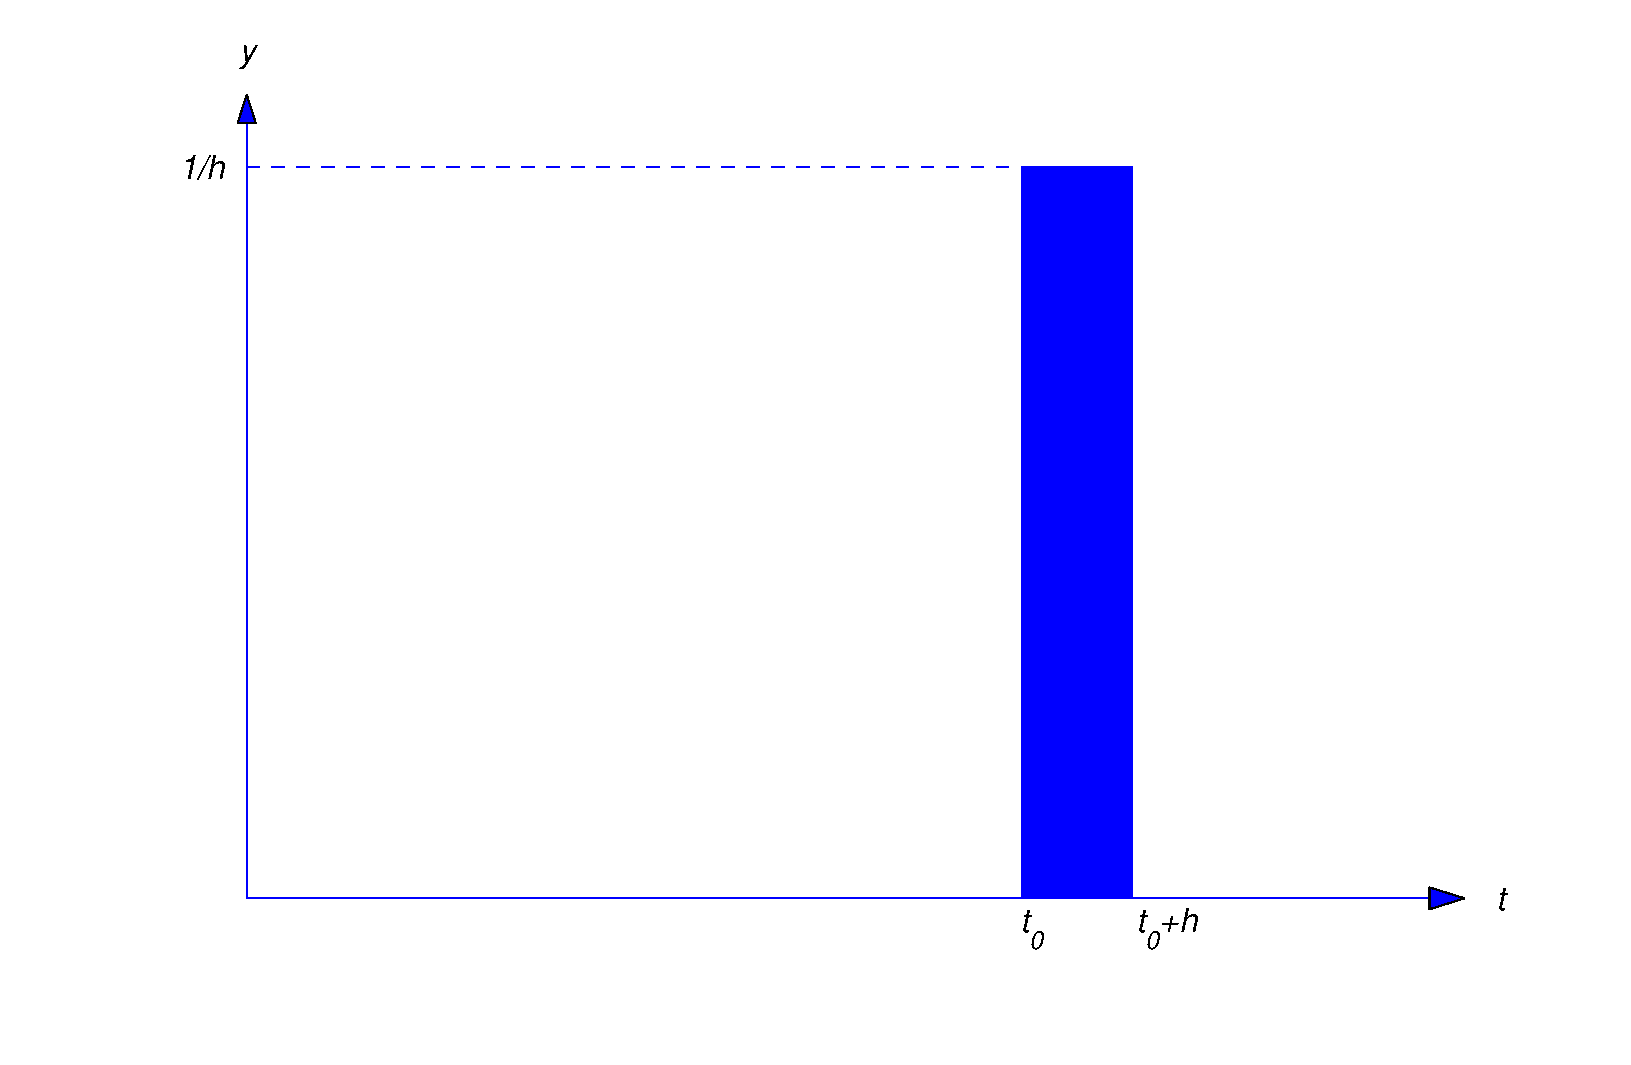
\includegraphics[bb=-78 148 689 643,width=5.67in,height=3.66in,keepaspectratio]{fig080701}
\caption{  $y=f_h(t)$}
  \label{figure:8.7.1}
\end{figure}

\proof
 Taking Laplace transforms in \eqref{eq:8.7.1} yields
$$
(as^2+bs+c)Y_h(s)=F_h(s),
$$
so
$$
Y_h(s)={F_h(s)\over as^2+bs+c}.
$$
The convolution theorem implies that
$$
y_h(t)=\int_0^t w(t-\tau)f_h(\tau)\,d\tau.
$$
Therefore,  \eqref{eq:8.7.2} implies that
\begin{equation} \label{eq:8.7.4}
y_h(t)=\left\{\begin{array}{cl} 0,&0\le t<t_0,\\[2\jot]
\dst{{1\over h}\int_{t_0}^tw(t-\tau)\,d\tau},&t_0\le t\le
t_0+h,\\[2\jot]
\dst{{1\over h
}\int_{t_0}^{t_0+h}w(t-\tau)\,d\tau},&t>t_0+h.\end{array}\right.
\end{equation}
Since $y_h(t)=0$ for all $h$ if $0\le t\le t_0$, it follows that
\begin{equation} \label{eq:8.7.5}
\lim_{h\to0+}y_h(t)=0\mbox{\quad if \quad}0\le t\le t_0.
\end{equation}
We'll now show that
\begin{equation} \label{eq:8.7.6}
\lim_{h\to0+}y_h(t)=w(t-t_0)\mbox{\quad if \quad}t>t_0.
\end{equation}

Suppose   $t$ is fixed and $t>t_0$.
From
\eqref{eq:8.7.4},
\begin{equation} \label{eq:8.7.7}
y_h(t)={1\over h}\int_{t_0}^{t_0+h}w(t-\tau)d\tau\mbox{\quad if \quad}
h<t-t_0.
\end{equation}
Since
\begin{equation} \label{eq:8.7.8}
{1\over h}\int_{t_0}^{t_0+h}d\tau=1,
\end{equation}
we can write
$$
w(t-t_0)={1\over h}w(t-t_0)\int_{t_0}^{t_0+h}\,d\tau=
{1\over h}\int_{t_0}^{t_0+h}w(t-t_0)\,d\tau.
$$
From this and \eqref{eq:8.7.7},
$$
y_h(t)-w(t-t_0)=
{1\over h}\int_{t_0}^{t_0+h}\left(w(t-\tau)-w(t-t_0)\right)\,d\tau.
$$
Therefore
\begin{equation} \label{eq:8.7.9}
|y_h(t)-w(t-t_0)|\le
{1\over h}\int_{t_0}^{t_0+h}|w(t-\tau)-w(t-t_0)|\,d\tau.
\end{equation}
Now let $M_h$ be the maximum value of $|w(t-\tau)-w(t-t_0)|$ as $\tau$
varies over the interval $[t_0,t_0+h]$. (Remember that $t$ and $t_0$
are fixed.) Then \eqref{eq:8.7.8} and \eqref{eq:8.7.9} imply that
\begin{equation} \label{eq:8.7.10}
|y_h(t)-w(t-t_0)|\le
{1\over h}M_h\int_{t_0}^{t_0+h}\,d\tau=M_h.
\end{equation}
But $\lim_{h\to0+}M_h=0$, since $w$ is continuous.
Therefore \eqref{eq:8.7.10} implies \eqref{eq:8.7.6}.
This and \eqref{eq:8.7.5} imply \eqref{eq:8.7.3}. \bbox

Theorem~\ref{thmtype:8.7.1} motivates the next definition.

\begin{definition}\color{blue}\label{thmtype:8.7.2} \rm
If $t_0>0$, then the solution of the initial value problem
\begin{equation} \label{eq:8.7.11}
ay''+by'+cy=\delta(t-t_0), \quad  y(0)=0,\quad y'(0)=0,
\end{equation}
is defined to be
$$
y=u(t-t_0)w(t-t_0),
$$
where
$$
w={\cal L}^{-1}\left(1\over as^2+bs+c\right).
$$
\end{definition}

In physical applications where the input $f$ and the output $y$ of a
device are related by the differential equation
$$
ay''+by'+cy=f(t),
$$
$w$ is called the {\color{blue}\it impulse response\/} of the device. Note
that
$w$ is the solution of the initial value problem
\begin{equation} \label{eq:8.7.12}
aw''+bw'+cw=0, \quad  w(0)=0,\quad  w'(0)=1/a,
\end{equation}
as can be seen by using the Laplace transform to solve this problem.
(Verify.)
On the other hand, we can solve \eqref{eq:8.7.12} by the methods of
Section~5.2 and show that $w$ is defined on
$(-\infty,\infty)$ by
\begin{equation} \label{eq:8.7.13}
w={e^{r_2t}-e^{r_1t}\over a(r_2-r_1)},\quad
w={1\over a}te^{r_1t}, \mbox{\quad or \quad}
w={1\over a\omega}e^{\lambda t}\sin\omega t,
\end{equation}
depending upon whether the polynomial $p(r)=ar^2+br+c$ has distinct
real zeros $r_1$ and $r_2$, a repeated zero $r_1$, or complex
conjugate zeros $\lambda\pm i\omega$. (In most physical applications,
the zeros of the characteristic polynomial have negative real parts,
so $\lim_{t\to\infty}w(t)=0$.) This means that $y=u(t-t_0)w(t-t_0)$ is
defined on $(-\infty,\infty)$ and has the following properties:
$$
y(t)=0,\quad  t<t_0,
$$
$$
ay''+by'+cy=0\mbox{\quad  on \quad }  (-\infty,t_0)\mbox{\quad and
\quad}(t_0,\infty),
$$
and
\begin{equation} \label{eq:8.7.14}
y'_-(t_0)=0, \quad   y'_+(t_0)=1/a
\end{equation}
(remember that $y'_-(t_0)$ and $y'_+(t_0)$ are derivatives from the
right and left, respectively) and $y'(t_0)$ does not exist. Thus, even
though we defined $y=u(t-t_0)w(t-t_0)$ to be the solution of
\eqref{eq:8.7.11},  this function {\color{blue}\it doesn't satisfy\/}
the differential equation in \eqref{eq:8.7.11} {\color{blue}\it at\/} $t_0$, since it
isn't differentiable there;   in fact \eqref{eq:8.7.14} indicates that an
impulse causes a jump discontinuity in velocity. (To see that this is
reasonable, think of what happens when you hit a ball with a bat.)
This means that the initial value problem \eqref{eq:8.7.11} doesn't make
sense if $t_0=0$, since $y'(0)$ doesn't exist in this case. However
$y=u(t)w(t)$ can be defined to be the solution of the modified initial
value problem
$$
ay''+by'+cy=\delta(t), \quad  y(0)=0,\quad y'_-(0)=0,
$$
where the condition on the derivative at $t=0$ has been replaced by a
condition on the derivative from the left.

Figure~\ref{figure:8.7.2} illustrates Theorem~\ref{thmtype:8.7.1} for the
case where the impulse response $w$ is the first expression in
\eqref{eq:8.7.13} and $r_1$ and $r_2$ are distinct and both negative. The
solid curve in the figure is the graph of $w$. The dashed curves are
solutions of \eqref{eq:8.7.1} for various values of $h$. As $h$ decreases
the graph of $y_h$ moves to the left toward the graph of $w$.

\begin{figure}[tbp]
  \centering\color{blue}
  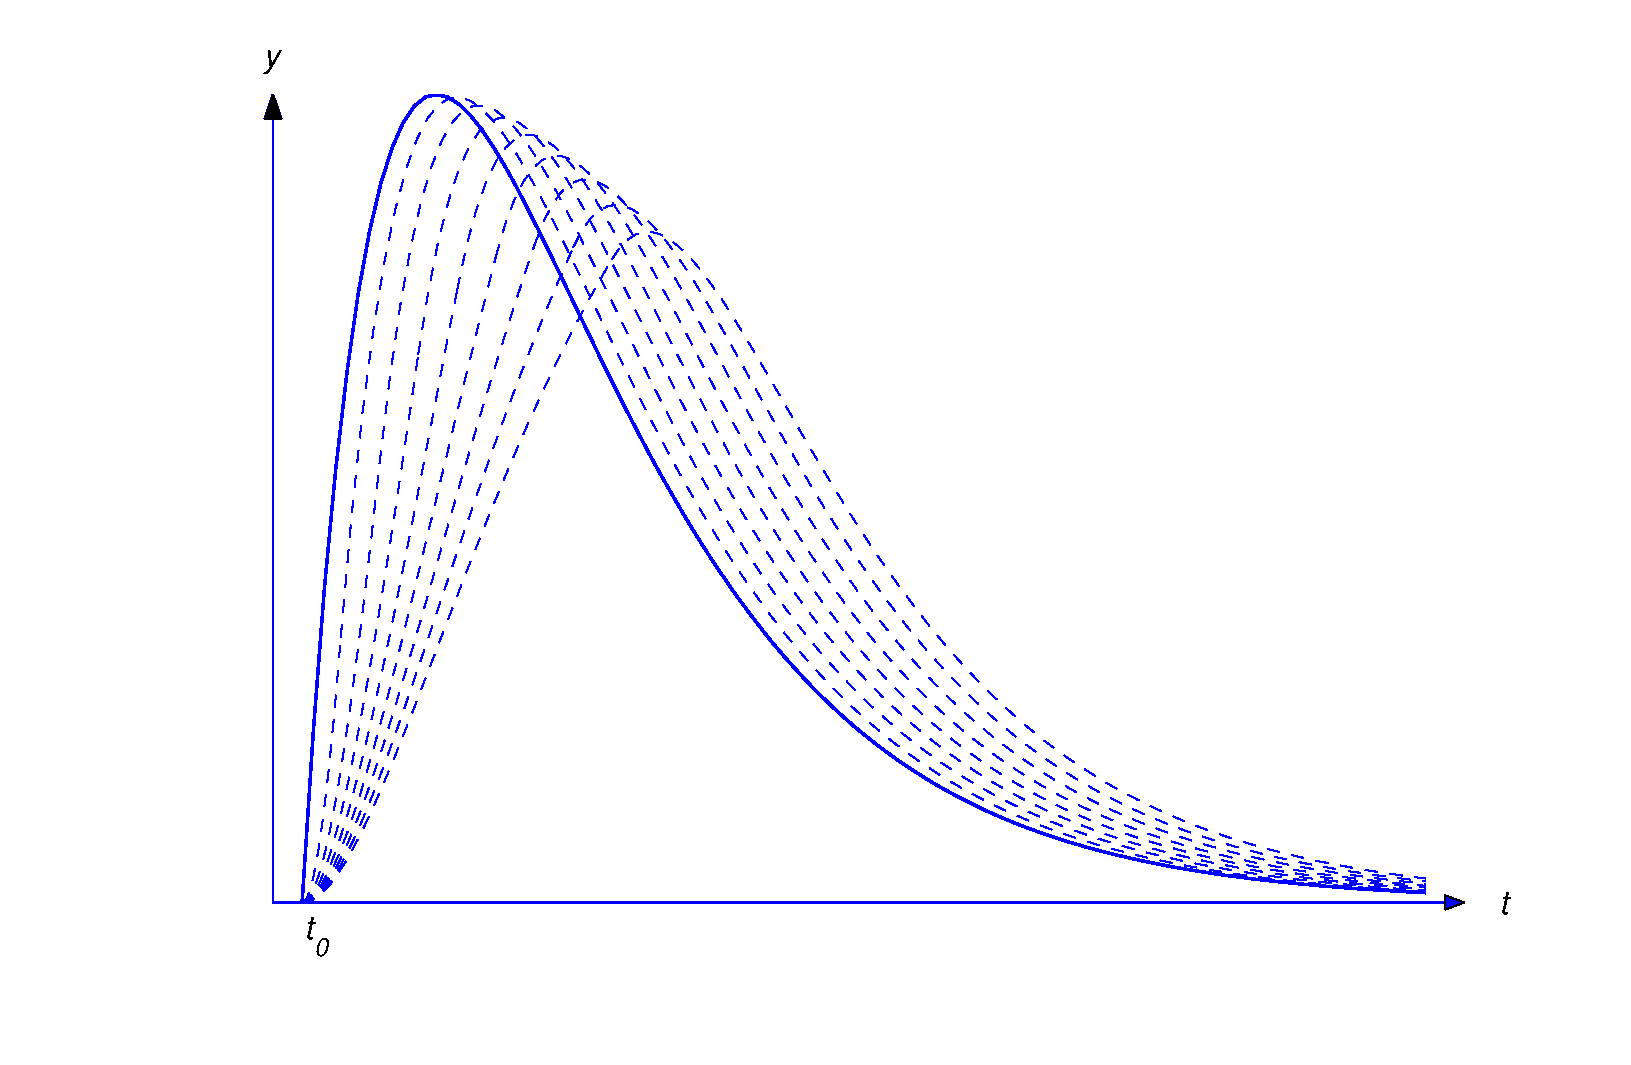
\includegraphics[bb=-78 148 689 643,width=5.67in,height=3.66in,keepaspectratio]{fig080702}
\caption{ An illustration of
Theorem~\ref{thmtype:8.7.1}}
  \label{figure:8.7.2}
\end{figure}

\begin{example}\label{example:8.7.1} \rm  Find the solution of the initial
value problem
\begin{equation} \label{eq:8.7.15}
y''-2y'+y=\delta(t-t_0), \quad  y(0)=0,\quad y'(0)=0,
\end{equation}
where $t_0>0$. Then interpret the solution for the case where $t_0=0$.
\end{example}

\solution
Here
$$
w={\cal L}^{-1}\left(1\over s^2-2s+1\right)={\cal L}^{-1}\left(
1\over(s-1)^2\right)=te^{-t},
$$
so  Definition~\ref{thmtype:8.7.2} yields
$$
y=u(t-t_0)(t-t_0)e^{-(t-t_0)}
$$
as the solution of  \eqref{eq:8.7.15} if $t_0>0$. If $t_0=0$,
then \eqref{eq:8.7.15} doesn't have a solution;     however,
$y=u(t)te^{-t}$
(which we would usually write simply as $y=te^{-t}$) is the solution
of the modified initial value problem
$$
y''-2y'+y=\delta(t), \quad  y(0)=0,\quad y_-'(0)=0.
$$

The graph of $y=u(t-t_0)(t-t_0)e^{-(t-t_0)}$ is shown in
Figure~\ref{figure:8.7.3} \bbox

\begin{figure}[tbp]
  \centering\color{blue}
  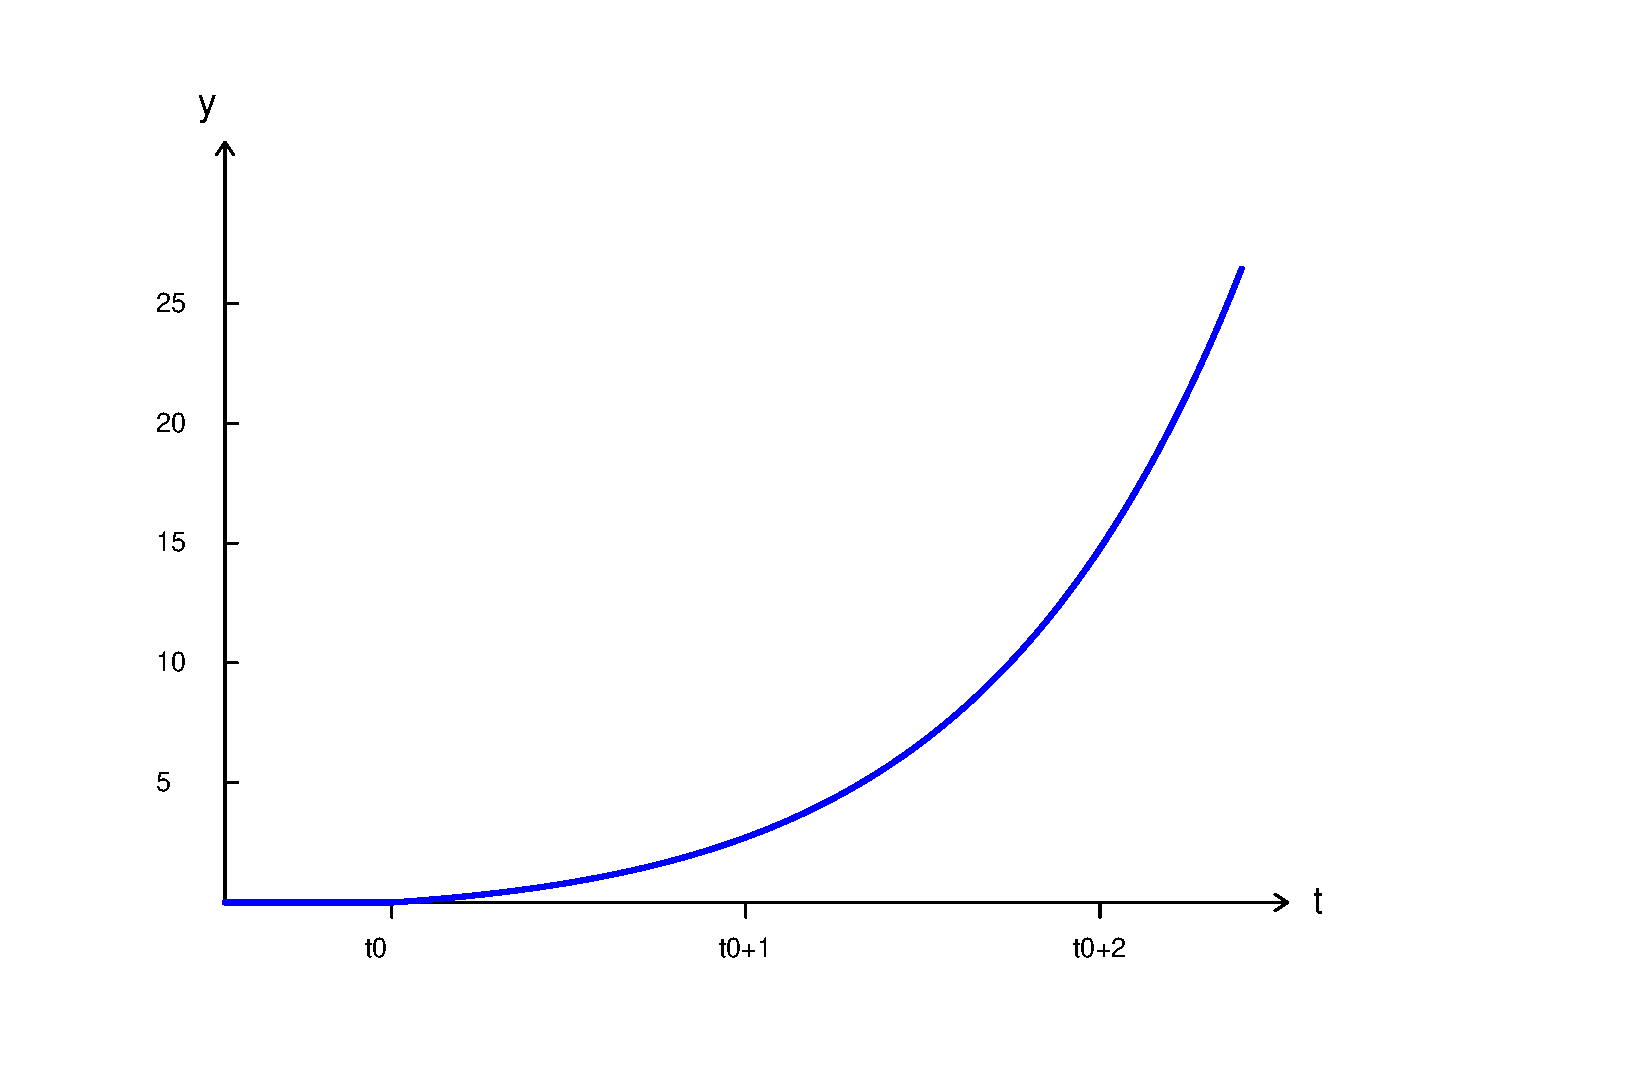
\includegraphics[bb=-78 148 689 643,width=5.67in,height=3.66in,keepaspectratio]{fig080703}
\caption{
$y=u(t-t_0)(t-t_0)e^{-(t-t_0)}$}
  \label{figure:8.7.3}
\end{figure}

Definition~\ref{thmtype:8.7.2} and the principle of superposition
motivate the next definition.

\begin{definition}\color{blue} \label{thmtype:8.7.3} \rm  Suppose
$\alpha$ is a nonzero constant and
$f$ is
piecewise continuous on $[0,\infty)$.
If $t_0>0$, then the solution of  the  initial value problem
$$
ay''+by'+cy=f(t)+\alpha\delta(t-t_0), \quad  y(0)=k_0,\quad y'(0)=k_1
$$
is defined to be
$$
y(t)=\hat y(t)+\alpha u(t-t_0)w(t-t_0),
$$
where $\hat y$  is the solution of
$$
ay''+by'+cy=f(t), \quad  y(0)=k_0,\quad y'(0)=k_1.
$$
This definition also applies if $t_0=0$, provided that the initial
condition $y'(0)=k_1$ is replaced by $y_-'(0)=k_1$.
\end{definition}

\begin{example}\label{example:8.7.2} \rm
Solve the initial value problem
\begin{equation} \label{eq:8.7.16}
y''+6y'+5y=3e^{-2t}+2\delta(t-1),\quad y(0)=-3,\quad y'(0)=2.
\end{equation}
\end{example}

\solution  We leave it to you to show that
the solution of
$$
y''+6y'+5y=3e^{-2t}, \quad    y(0)=-3,\;   y'(0)=2
$$
is
$$
\hat y=-e^{-2t}+{1\over2}e^{-5t}-{5\over2}e^{-t}.
$$
Since
$$
\begin{array}{ccccl}
w(t)&=&{\cal L}^{-1}\left(\dst{1\over s^2+6s+5}\right)&=&
{\cal L}^{-1}\left(\dst{1\over(s+1)(s+5)}\right)\\[2\jot]
&=&\dst{{1\over4}{\cal L}^{-1}\left({1\over s+1}-{1\over s+5}\right)}
&=&\dst{e^{-t}-e^{-5t}\over4},
\end{array}
$$
the solution of  \eqref{eq:8.7.16} is
\begin{equation} \label{eq:8.7.17}
y=-e^{-2t}+{1\over2}e^{-5t}-{5\over2}e^{-t}
+u(t-1){e^{-(t-1)}-e^{-5(t-1)}\over2}
\end{equation}
(Figure~\ref{figure:8.7.4})\bbox.

\begin{figure}[htbp]
\color{blue}
  \begin{minipage}[b]{0.5\linewidth}
    \centering
   \scalebox{.65}{
  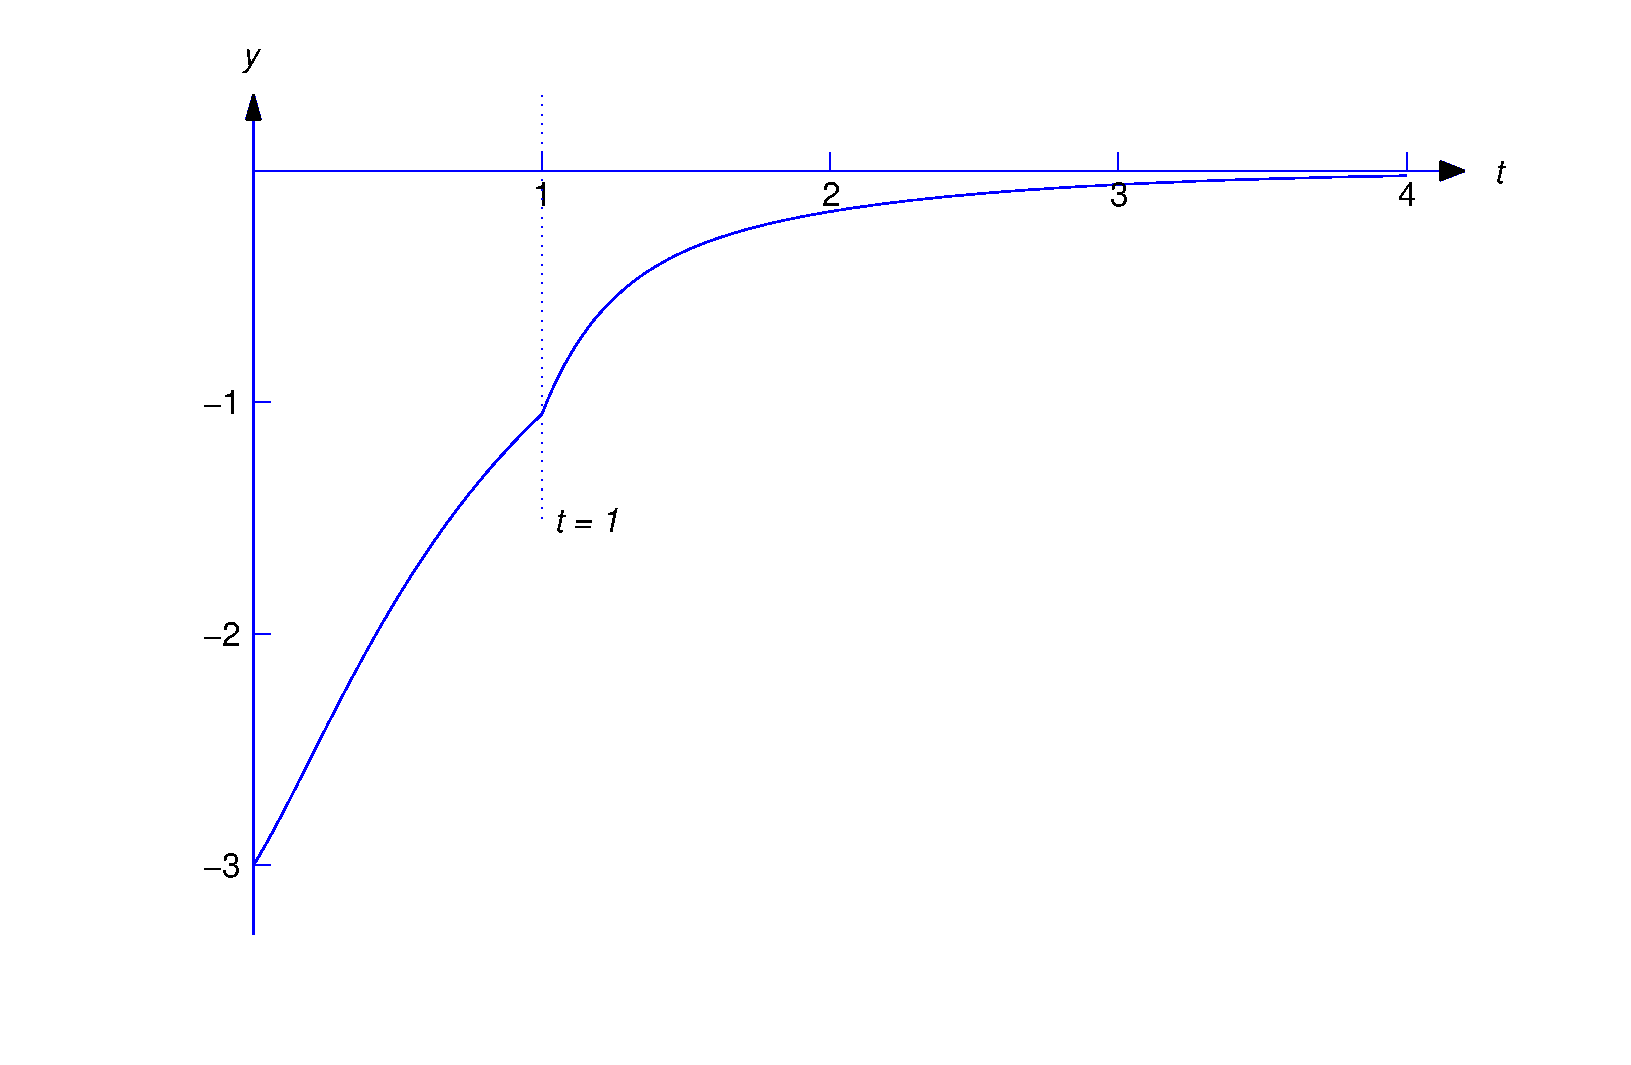
\includegraphics[bb=-78 148 689 643,width=5.67in,height=3.66in,keepaspectratio]{fig080704}}
\caption{ Graph of \eqref{eq:8.7.17}}
  \label{figure:8.7.4}
\end{minipage}
  \begin{minipage}[b]{0.5\linewidth}
    \centering
   \scalebox{.65}{
  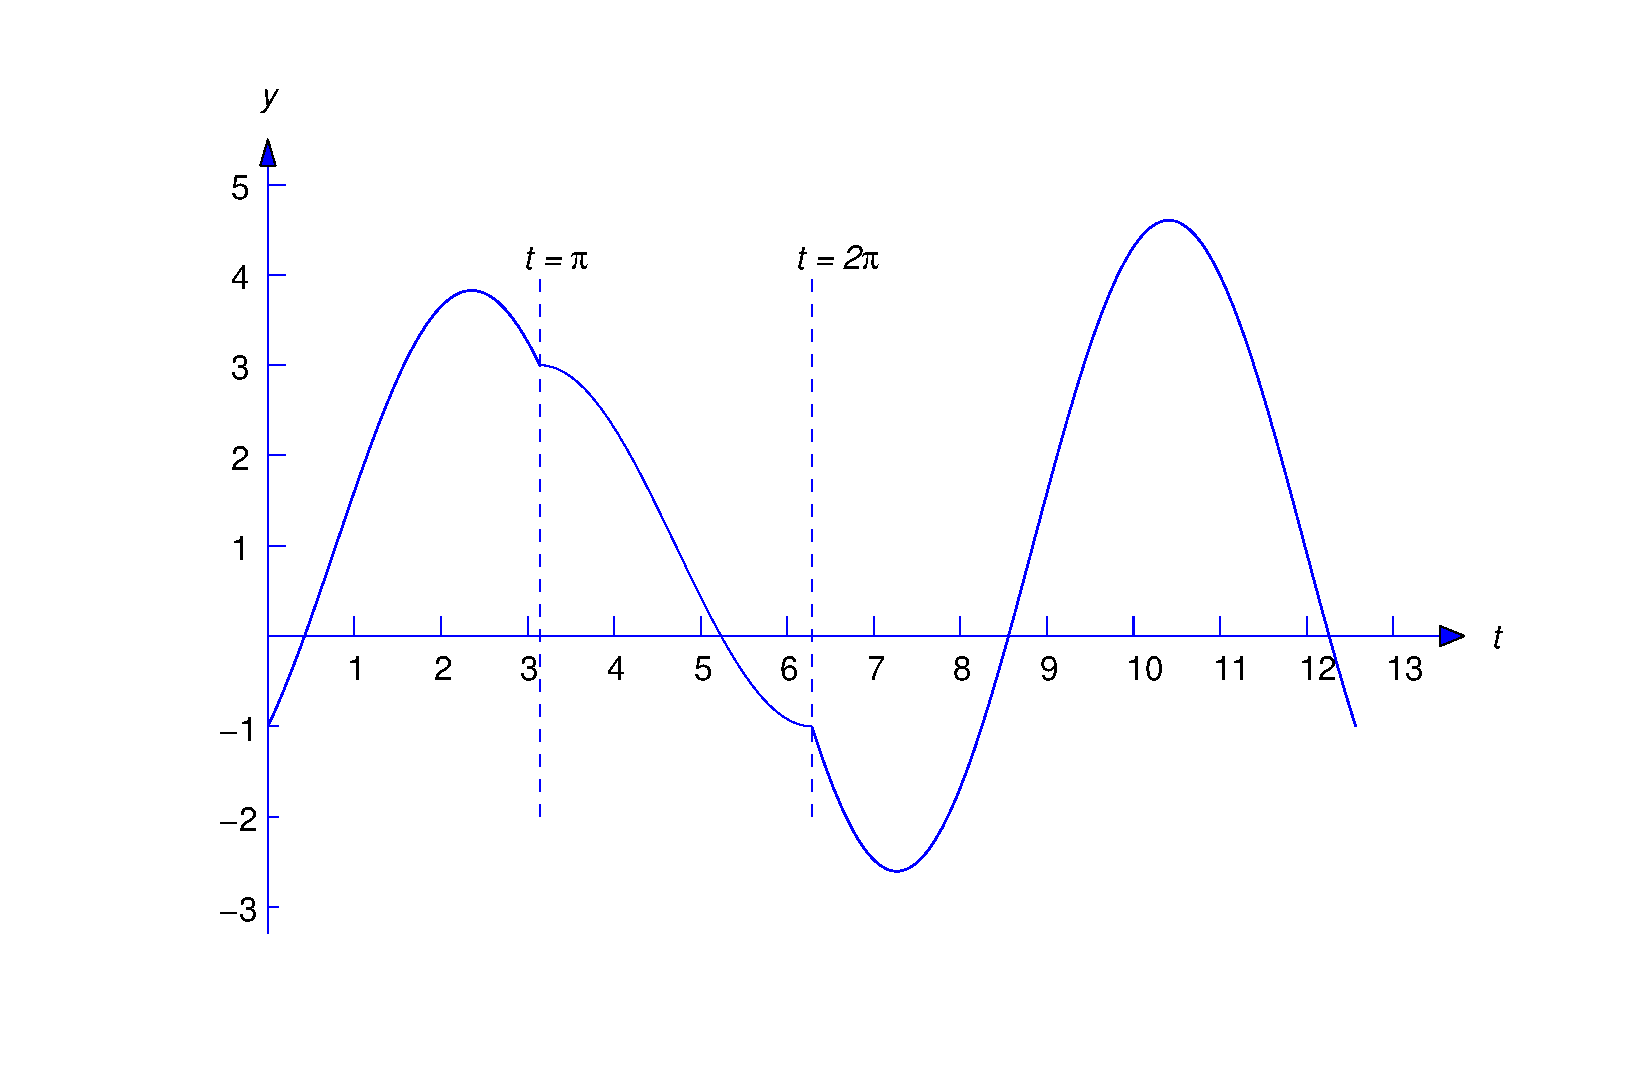
\includegraphics[bb=-78 148 689 643,width=5.67in,height=3.66in,keepaspectratio]{fig080705}}
\caption{ Graph of \eqref{eq:8.7.19}}
  \label{figure:8.7.5}
\end{minipage}
\end{figure}

Definition~\ref{thmtype:8.7.3} can be extended in the obvious way to cover
the case where the forcing function contains more than one impulse.
\begin{example}\label{example:8.7.3} \rm
Solve the  initial value problem
\begin{equation} \label{eq:8.7.18}
y''+y=1+2\delta(t-\pi)-3\delta(t-2\pi), \quad    y(0)=-1,\;   y'(0)=2.
\end{equation}
\end{example}

\solution
We leave it to you to show that
$$
\hat y= 1-2\cos t+2\sin t
$$
is the solution of
$$
y''+y=1, \quad    y(0)=-1,\quad    y'(0)=2.
$$
Since
$$
w={\cal L}^{-1}\left(1\over s^2+1\right)=\sin t,
$$
the solution of  \eqref{eq:8.7.18} is
\begin{eqnarray*}
y&=&1-2\cos t+2\sin t+2u(t-\pi)\sin(t-\pi)-3u(t-2\pi)\sin(t-2\pi)\\
&=&1-2\cos t+2\sin t-2u(t-\pi)\sin t-3u(t-2\pi)\sin t,
\end{eqnarray*}
or
\begin{equation} \label{eq:8.7.19}
y=\left\{\begin{array}{cl} 1-2\cos t+2\sin t,&0\le t<\pi,\\[5pt]
1-2\cos t,&\pi\le t<2\pi,\\[5pt]
1-2\cos t-3\sin t,&t\ge 2\pi\end{array}\right.
\end{equation}
(Figure~\ref{figure:8.7.5}).

\newpage

\exercises
In Exercises~\ref{exer:8.7.1}--\ref{exer:8.7.20} solve the initial value
problem. Where indicated by \CGex, graph the solution.

\begin{exerciselist}
\item\label{exer:8.7.1}
 $y''+3y'+2y=6e^{2t}+2\delta(t-1), \quad  y(0)=2,\quad y'(0)=-6$

\item\label{exer:8.7.2} \CGex
 $y''+y'-2y=-10e^{-t}+5\delta(t-1), \quad  y(0)=7,\quad y'(0)=-9$

\item\label{exer:8.7.3}
 $y''-4y=2e^{-t}+5\delta(t-1), \quad  y(0)=-1,\quad y'(0)=2$

\item\label{exer:8.7.4}  \CGex
 $y''+y=\sin3t+2\delta(t-\pi/2), \quad  y(0)=1,\quad y'(0)=-1$

\item\label{exer:8.7.5}
 $y''+4y=4+\delta(t-3\pi), \quad  y(0)=0,\quad y'(0)=1$

\item\label{exer:8.7.6}
 $y''-y=8+2\delta(t-2), \quad  y(0)=-1,\quad y'(0)=1$

\item\label{exer:8.7.7}
 $y''+y'=e^t+3\delta(t-6), \quad  y(0)=-1,\quad y'(0)=4$

\item\label{exer:8.7.8}
 $y''+4y=8e^{2t}+\delta(t-\pi/2), \quad  y(0)=8,\quad y'(0)=0$

\item\label{exer:8.7.9} \CGex
 $y''+3y'+2y=1+\delta(t-1), \quad  y(0)=1,\quad y'(0)=-1$

\item\label{exer:8.7.10}
 $y''+2y'+y=e^t+2\delta(t-2), \quad  y(0)=-1,\quad y'(0)=2$

\item\label{exer:8.7.11} \CGex
 $y''+4y=\sin t+\delta(t-\pi/2), \quad  y(0)=0,\quad y'(0)=2$

\item\label{exer:8.7.12}
 $y''+2y'+2y=\delta(t-\pi)-3\delta(t-2\pi), \quad  y(0)=-1,\quad y'(0)=2$

\item\label{exer:8.7.13}
$y''+4y'+13y=\delta(t-\pi/6)+2\delta(t-\pi/3), \quad  y(0)=1,\quad y'(0)=2$

\item\label{exer:8.7.14}
$2y''-3y'-2y=1+\delta(t-2), \quad  y(0)=-1,\quad y'(0)=2$

\item\label{exer:8.7.15}
$4y''-4y'+5y=4\sin t-4\cos
t+\delta(t-\pi/2)-\delta(t-\pi), \quad  y(0)=1,\quad y'(0)=1$

\item\label{exer:8.7.16}
$y''+y=\cos2t+2\delta(t-\pi/2)-3\delta(t-\pi), \quad  y(0)=0,\quad y'(0)=-1$

\item\label{exer:8.7.17} \CGex
$y''-y=4e^{-t}-5\delta(t-1)+3\delta(t-2), \quad  y(0)=0,\quad y'(0)=0$

\item\label{exer:8.7.18}
$y''+2y'+y=e^t-\delta(t-1)+2\delta(t-2), \quad  y(0)=0,\quad y'(0)=-1$

\item\label{exer:8.7.19}
$y''+y=f(t)+\delta(t-2\pi), \quad  y(0)=0,\quad y'(0)=1$, \text{and}

$f(t)=\dst{\left\{\begin{array}{cl}
\sin2t,&0\le t<\pi,\\[5pt]0,&t\ge \pi.\end{array}\right.}$

\item\label{exer:8.7.20}
$y''+4y=f(t)+\delta(t-\pi)-3\delta(t-3\pi/2), \quad  y(0)=1,\quad
y'(0)=-1$, \text {and}

$f(t)=\dst{\left\{\begin{array}{cl}1,&0\le t<\pi/2,\\[5pt]2,&t\ge
\pi/2\end{array}\right.}$

\item\label{exer:8.7.21}
$y''+y=\delta(t), \quad  y(0)=1,\quad y_-'(0)=-2$

\item\label{exer:8.7.22}
$y''-4y=3\delta(t), \quad  y(0)=-1,\quad y_-'(0)=7$

\item\label{exer:8.7.23}
$y''+3y'+2y=-5\delta(t), \quad  y(0)=0,\quad y_-'(0)=0$

\item\label{exer:8.7.24}
$y''+4y'+4y=-\delta(t), \quad  y(0)=1,\quad y_-'(0)=5$

\item\label{exer:8.7.25}
$4y''+4y'+y=3\delta(t), \quad  y(0)=1,\quad y_-'(0)=-6$

\exercisetext{
In Exercises~\ref{exer:8.7.26}-\ref{exer:8.7.28}, solve the initial value
problem
$$
ay_h''+by_h'+cy_h=
\left\{\begin{array}{cl} 0,&0\le t<t_0,\\[2\jot]
1/h,&t_0\le t< t_0+h,\\[2\jot]
0,&t\ge t_0+h,\end{array}\right.
\quad y_h(0)=0,\quad y_h'(0)=0,
$$
where $t_0>0$ and $h>0$. Then find
$$
w={\cal L}^{-1}\left(1\over as^2+bs+c\right)
$$
and verify Theorem~\ref{thmtype:8.7.1} by graphing $w$ and $y_h$
on the same axes, for small positive values of $h$.}

\item\label{exer:8.7.26} \Lex
$y''+2y'+2y=f_h(t), \quad  y(0)=0,\quad y'(0)=0$

\item\label{exer:8.7.27} \Lex
$y''+2y'+y=f_h(t), \quad  y(0)=0,\quad y'(0)=0$

\item\label{exer:8.7.28} \Lex
$y''+3y'+2y=f_h(t), \quad  y(0)=0,\quad y'(0)=0$

\item\label{exer:8.7.29}

Recall from Section~6.2 that the displacement of
an
object of mass $m$ in a spring--mass system in free damped oscillation is
$$
my''+cy'+ky=0, \quad  y(0)=y_0,\quad y'(0)=v_0,
$$
and that $y$ can be written as
$$
y=Re^{-ct/2m}\cos(\omega_1t-\phi)
$$
if the motion is underdamped. Suppose $y(\tau)=0$.
Find the impulse that would have to be applied to the object at $t=\tau$
 to put it in equilibrium.

\item\label{exer:8.7.30} Solve the initial value problem. Find a formula that
does not involve step functions and represents $y$  on each subinterval of
$[0,\infty)$  on which the forcing function is zero.

{\bf (a)} $\dst{y''-y=\sum_{k=1}^\infty\delta(t-k), \quad  y(0)=0,\quad y'(0)=1}$

{\bf (b)}
$\dst{y''+y=\sum_{k=1}^\infty\delta(t-2k\pi), \quad  y(0)=0,\quad y'(0)=1}$

{\bf (c)}
$\dst{y''-3y'+2y=\sum_{k=1}^\infty\delta(t-k), \quad  y(0)=0,\quad y'(0)=1}$

{\bf (d)}
$\dst{y''+y=\sum_{k=1}^\infty\delta(t-k\pi), \quad  y(0)=0,\quad y'(0)=0}$

\end{exerciselist}


\newpage

\section{A Brief Table of Laplace Transforms}

\begin{center}
  \begin{tabular}{ccc}
    {$f(t)$}                    & {$F(s)$}                                                         & {}             \\[15pt]
    1                           & $\displaystyle{\frac{1}{s}}$                                     & $(s>0)$        \\[15pt]
    $t^{n}$                     & $\displaystyle{\frac{n!}{s^{n+1}}}$                              & $(s>0)$        \\
    ($n=\mbox{ integer }>0$)    & {}                                                               & {}             \\[15pt]
    $t^{p},\;p>-1$              & $\displaystyle{\frac{\Gamma(p+1)}{s^{(p+1)}}}$                   & $(s>0)$        \\[15pt]
    $e^{at}$                    & $\displaystyle{\frac{1}{s-a}}$                                   & $(s>a)$        \\[15pt]
    $t^{n}e^{at}$               & $\displaystyle{\frac{n!}{(s-a)^{n+1}}}$                          & $(s> a)$        \\[15pt]
    ($n=\mbox{ integer }>0$)    & {}                                                               & {}             \\
    $\cos\omega t$              & $\displaystyle{\frac{s}{s^{2}+\omega^{2}}}$                      & $(s>0)$        \\[15pt]
    $\sin\omega t$              & $\displaystyle{\frac{\omega}{s^{2}+\omega^{2}}}$                 & $(s>0)$        \\[15pt]
    $e^{\lambda t}\cos\omega t$ & $\displaystyle{\frac{s-\lambda}{(s-\lambda)^{2}+\omega^{2}}}$    & $(s> \lambda)$ \\[15pt]
    $e^{\lambda t}\sin\omega t$ & $\displaystyle{\frac{\omega}{(s-\lambda)^{2}+\omega^{2}}}$       & $(s> \lambda)$ \\[15pt]
    $\cosh bt$                  & $\displaystyle{\frac{s}{s^{2}-b^{2}}}$                           & $(s>|b|)$      \\[15pt]
    $\sinh bt$                  & $\displaystyle{\frac{b}{s^{2}-b^{2}}}$                           & $(s>|b|)$      \\[15pt]
    $t\cos\omega t$             & $\displaystyle{\frac{s^{2}-\omega^{2}}{(s^{2}+\omega^{2})^{2}}}$ & $(s>0)$
  \end{tabular}
\end{center}

\begin{center}
  \begin{tabular}{ccc}
    $t\sin\omega t$                                      & $\displaystyle{\frac{2\omega s}{(s^{2}+\omega^{2})^{2}}}$                     & $(s>0)$ \\[15pt]
    $\sin\omega t-\omega t\cos\omega t$                  & $\displaystyle{\frac{2\omega^{3}}{(s^{2}+\omega^{2})^{2}}}$                   & $(s>0)$ \\[15pt]
    $\omega t-\sin\omega t$                              & $\displaystyle{\frac{\omega^{3}}{s^{2}(s^{2}+\omega^{2})}}$               & $(s>0)$ \\[15pt]
    $\displaystyle{\frac{1}{t}\sin\omega t}$             & $\displaystyle{\arctan\left(\frac{\omega}{s}\right)}$                         & $(s>0)$ \\[15pt]
    $e^{at}f(t)$                                         & $F(s-a)$                                                                      &         \\[15pt]
    $t^{k}f(t)$                                          & $\displaystyle{{(-1)^{k}F^{(k)}(s)}}$                                         &         \\[15pt]
    $f(\omega t)$                                        & $\displaystyle{\frac{1}{\omega}F\left(\frac{s}{\omega}\right),\quad\omega>0}$ &         \\[15pt]
    $u(t-\tau)$                                          & $\displaystyle{\frac{e^{-\tau s}}{s}}$                                        & $(s>0)$ \\[15pt]
    $u(t-\tau)f(t-\tau)\,(\tau>0)$                       & $e^{-\tau s}F(s)$                                                             &         \\[15pt]
    $\displaystyle{\int^{t}_{0}f(\tau)g(t-\tau)\,d\tau}$ & $F(s)\cdot G(s)$                                                              &         \\[15pt]
    $\delta(t-a)$                                        & $e^{-as}$                                                                     & $(s>0)$ \\[15pt]
  \end{tabular}
\end{center}

